\documentclass[compress]{beamer}

\usetheme{Luebeck}
\usepackage[utf8]{inputenc}
\usepackage{subfig}
\usepackage{utopia} %font utopia imported
\usepackage{arabtex}
\usepackage{utf8}
\setcode{utf8}
\usepackage{amsmath}
\usepackage{amssymb}
\usepackage{amsthm}
\usepackage{textcomp}
\usefonttheme{professionalfonts} % using non standard fonts for beamer
\definecolor{foo}{RGB}{106,141,143}
\usecolortheme[named=foo]{structure}
\setbeamercolor{subsection in head/foot}{bg=foo!80!black}
% This block of code defines the information to appear in the
% title page

\title[ASIC Physical Design] %optional
{Clock Tree Synthesis}

\subtitle{How to Synchronize your own chip}

\author[Ahmed Abdelazeem] % (optional)
{Ahmed Abdelazeem}
%{A.~B.~Arthur\inst{1} \and J.~Doe\inst{2}}

\institute[ZU] % (optional)
{
	Faculty of Engineering\\
	Zagazig University
}
%{
	%	\inst{1}%
	%	Faculty of Engineering\\
	%	Zagazig University
	%	\and
	%	\inst{2}%
	%	Faculty of Chemistry\\
	%	Very Famous University
	%}

\date[ZU 2023] % (optional)
{RTL2GDSII Flow, March 2022}

%\logo{
\includegraphics[height=1.5cm]{lion-logo.png}}

%End of title page configuration block
%------------------------------------------------------------

%------------------------------------------------------------
%The next block of commands puts the table of contents at the
%beginning of each section and highlights the current section:
\setcounter{tocdepth}{1} %%%
\AtBeginSection[]
{
	\begin{frame}
		\frametitle{Table of Contents}
		\tableofcontents[currentsection]
	\end{frame}
}
%------------------------------------------------------------


\begin{document}
	
	%The next statement creates the title page.
	\frame{\titlepage}
	
	
	%---------------------------------------------------------
	%This block of code is for the table of contents after
	%the title page
	\begin{frame}
		\frametitle{Table of Contents}
		\tableofcontents
	\end{frame}
	%---------------------------------------------------------
%--------------------------------------------------
\section[Intro]{Introduction}
\subsection[CTS]{Clock Tree Synthesis}
\begin{frame}
	\frametitle{Design Status, Start of CTS Phase}
	\begin{itemize}
		\item Placement - completed
		\item Power and ground nets – prerouted
		\item Estimated congestion - acceptable
		\item Estimated timing - acceptable (~0ns slack)
		\item Estimated max cap/transition – no violations
		\item High fanout nets:
			\begin{enumerate}
				\item Reset, Scan Enable synthesized with buffers
				\item Clocks are still not buffered
			\end{enumerate}
	\end{itemize}
\pause
\begin{alertblock}{Question}
Why are there no buffers on clock nets?
\end{alertblock}
\end{frame}	
\subsection[CTS]{CTS Problem}
\begin{frame}
	\frametitle{CTS Problem}
		\begin{itemize}
			\item \textcolor{red}{CTS is the process of distributing clock signals to clock pins based on physical/layout information}
			\item After placement of cells the tree of synchronization is synthesized
			\item Balanced clock tree is synchronized with the addition of buffers
			\item After routing CT optimization is made
		\end{itemize}
		
		\begin{center}
			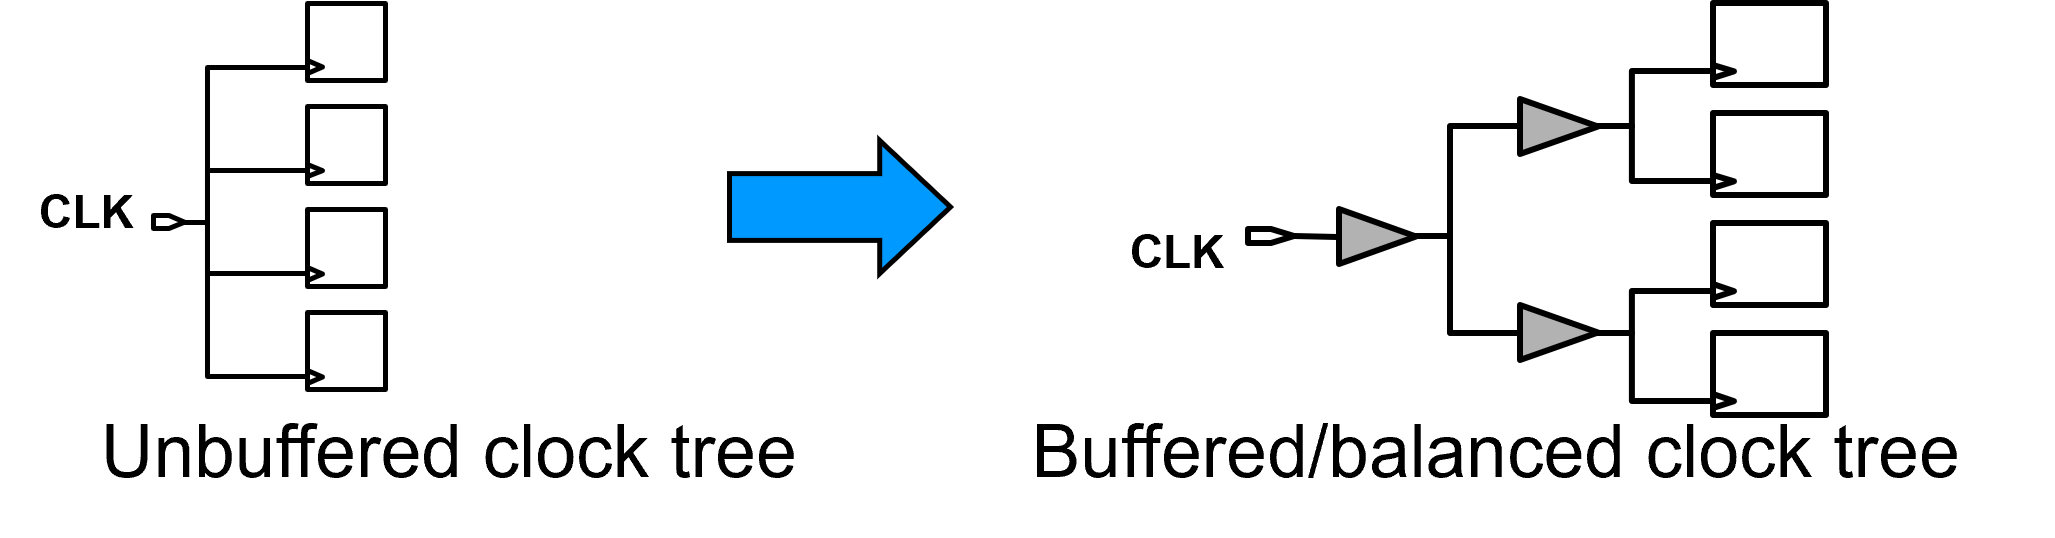
\includegraphics[width=0.7\textwidth]{CTS}
		\end{center}
	
\end{frame}

\begin{frame}
	\frametitle{Starting Point before CTS}
		\begin{itemize}
			\item All clock pins are driven by a single clock source
			\item All clock pins are from a source of clock pulses in various geometrical distances		
		\end{itemize}
	\begin{center}
	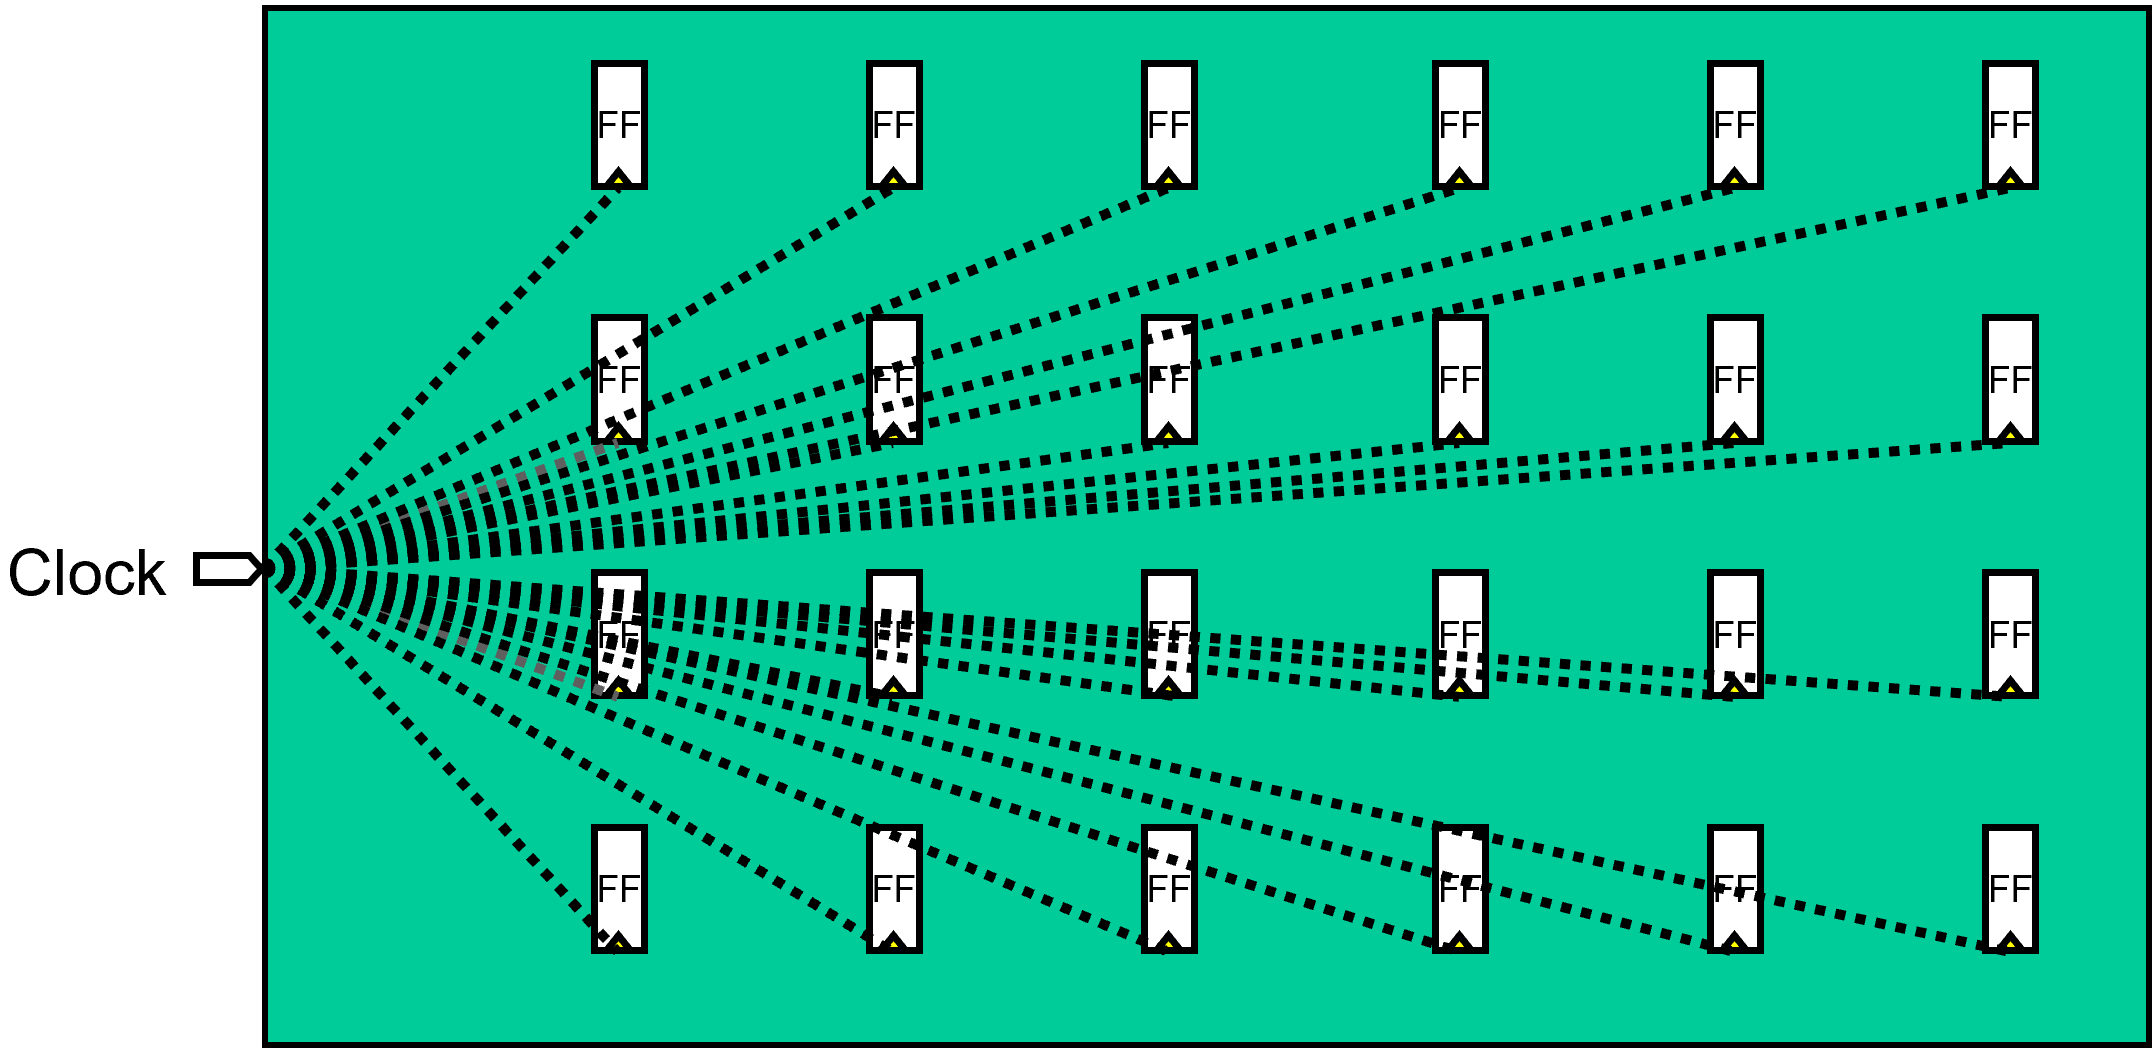
\includegraphics[width=0.8\textwidth]{CTS1}
\end{center}
		
\end{frame}
\begin{frame}
	\frametitle{CTS Goals}
	\begin{center}
		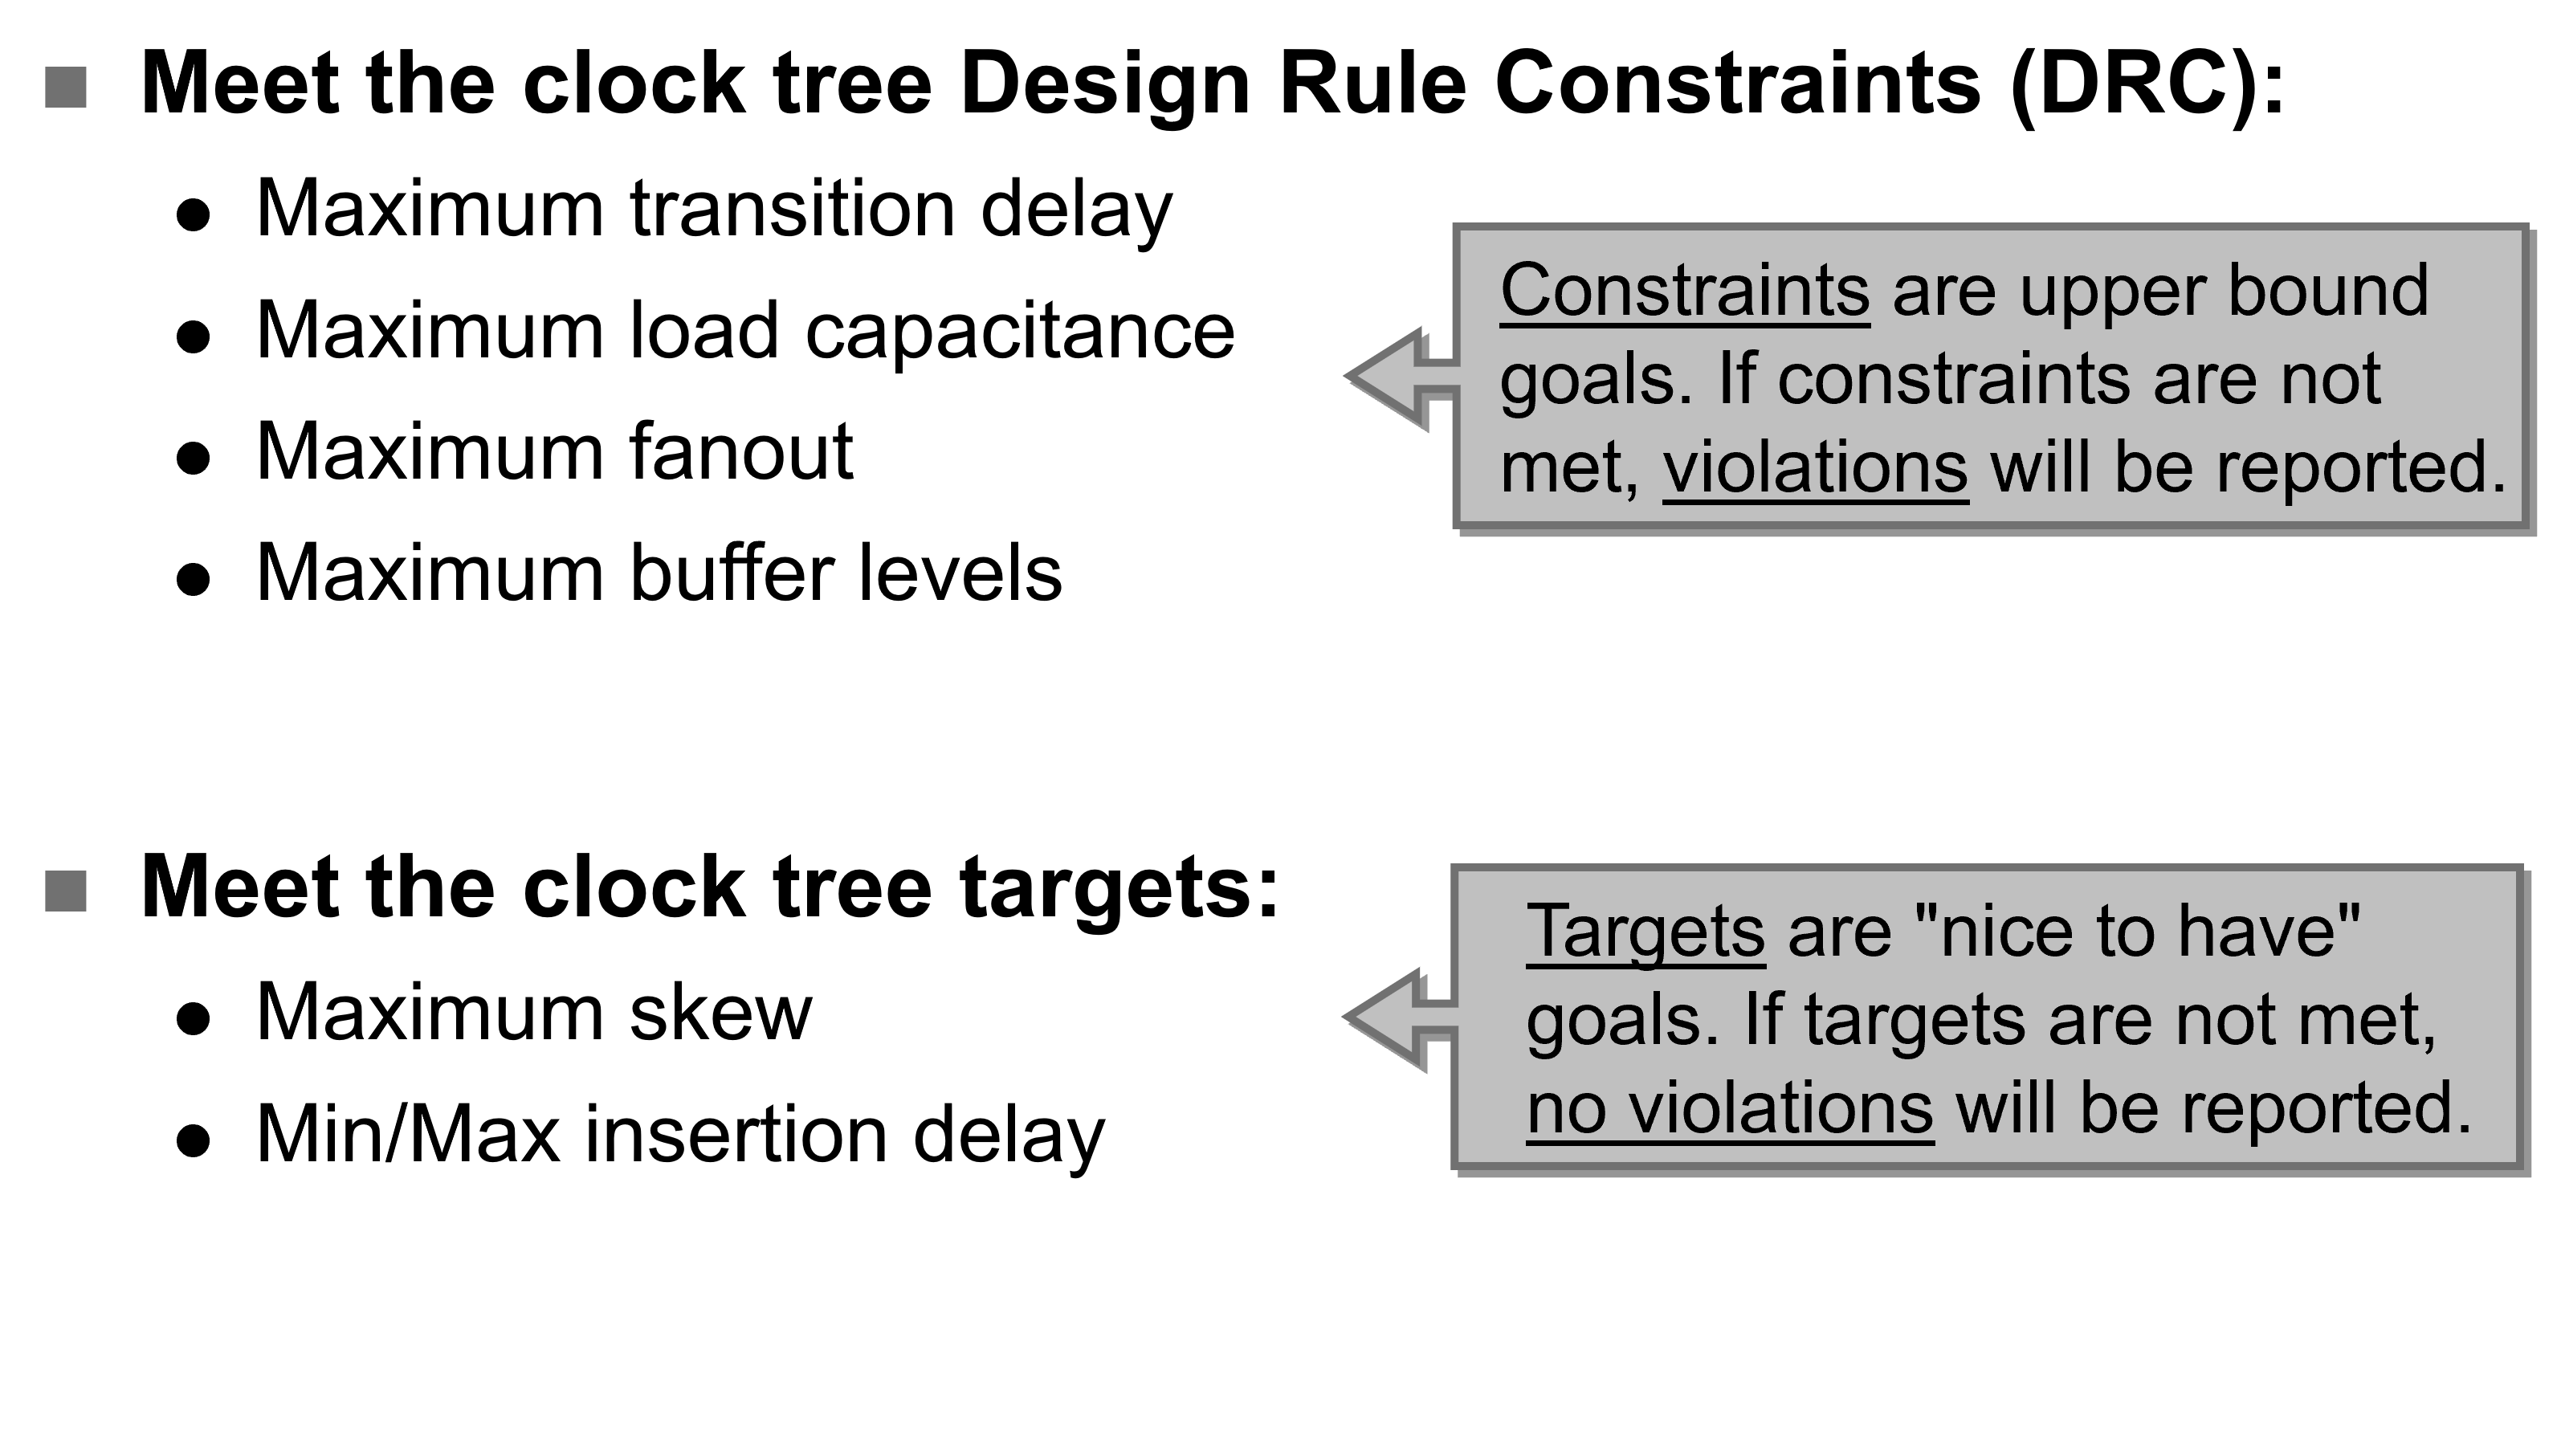
\includegraphics[width=\textwidth]{GOALS}
	\end{center}
\end{frame}

\begin{frame}
	\frametitle{Clock Tree Synthesis (CTS) (1/2)}
		\begin{center}
			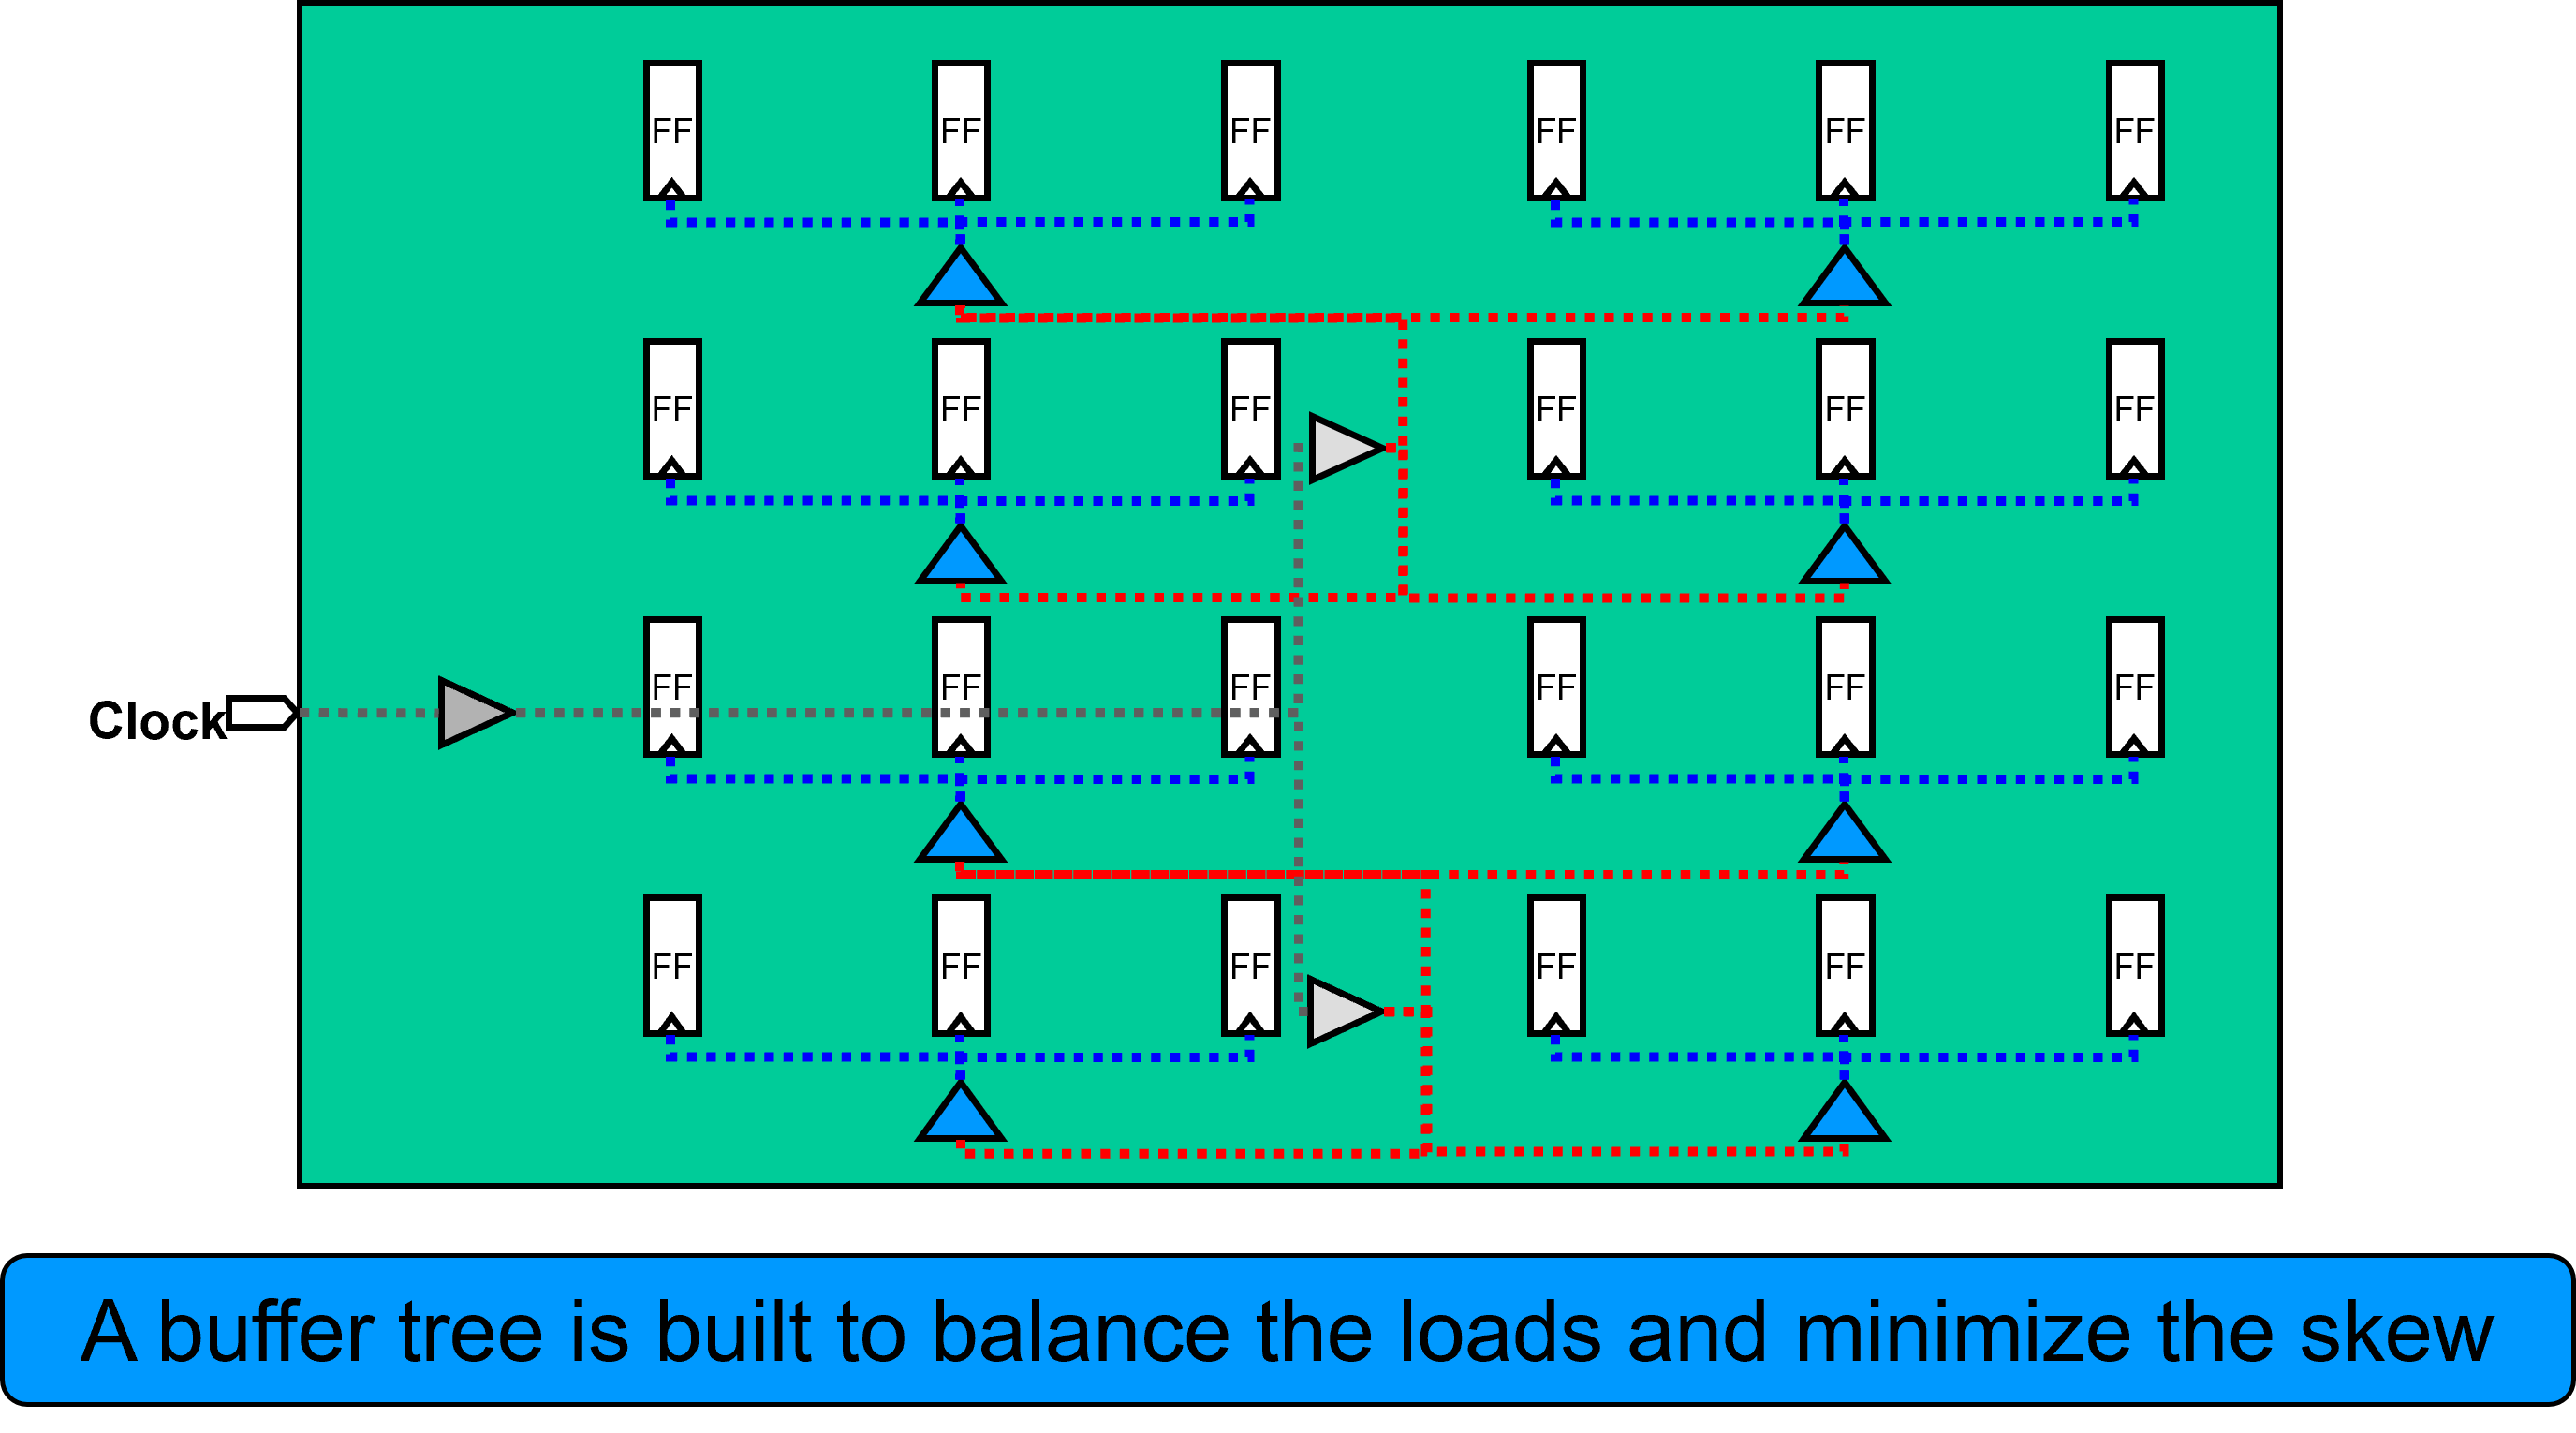
\includegraphics[width=\textwidth]{CTS2}
		\end{center}
\end{frame}
\begin{frame}
	\frametitle{Clock Tree Synthesis (CTS) (2/2)}
	\begin{center}
		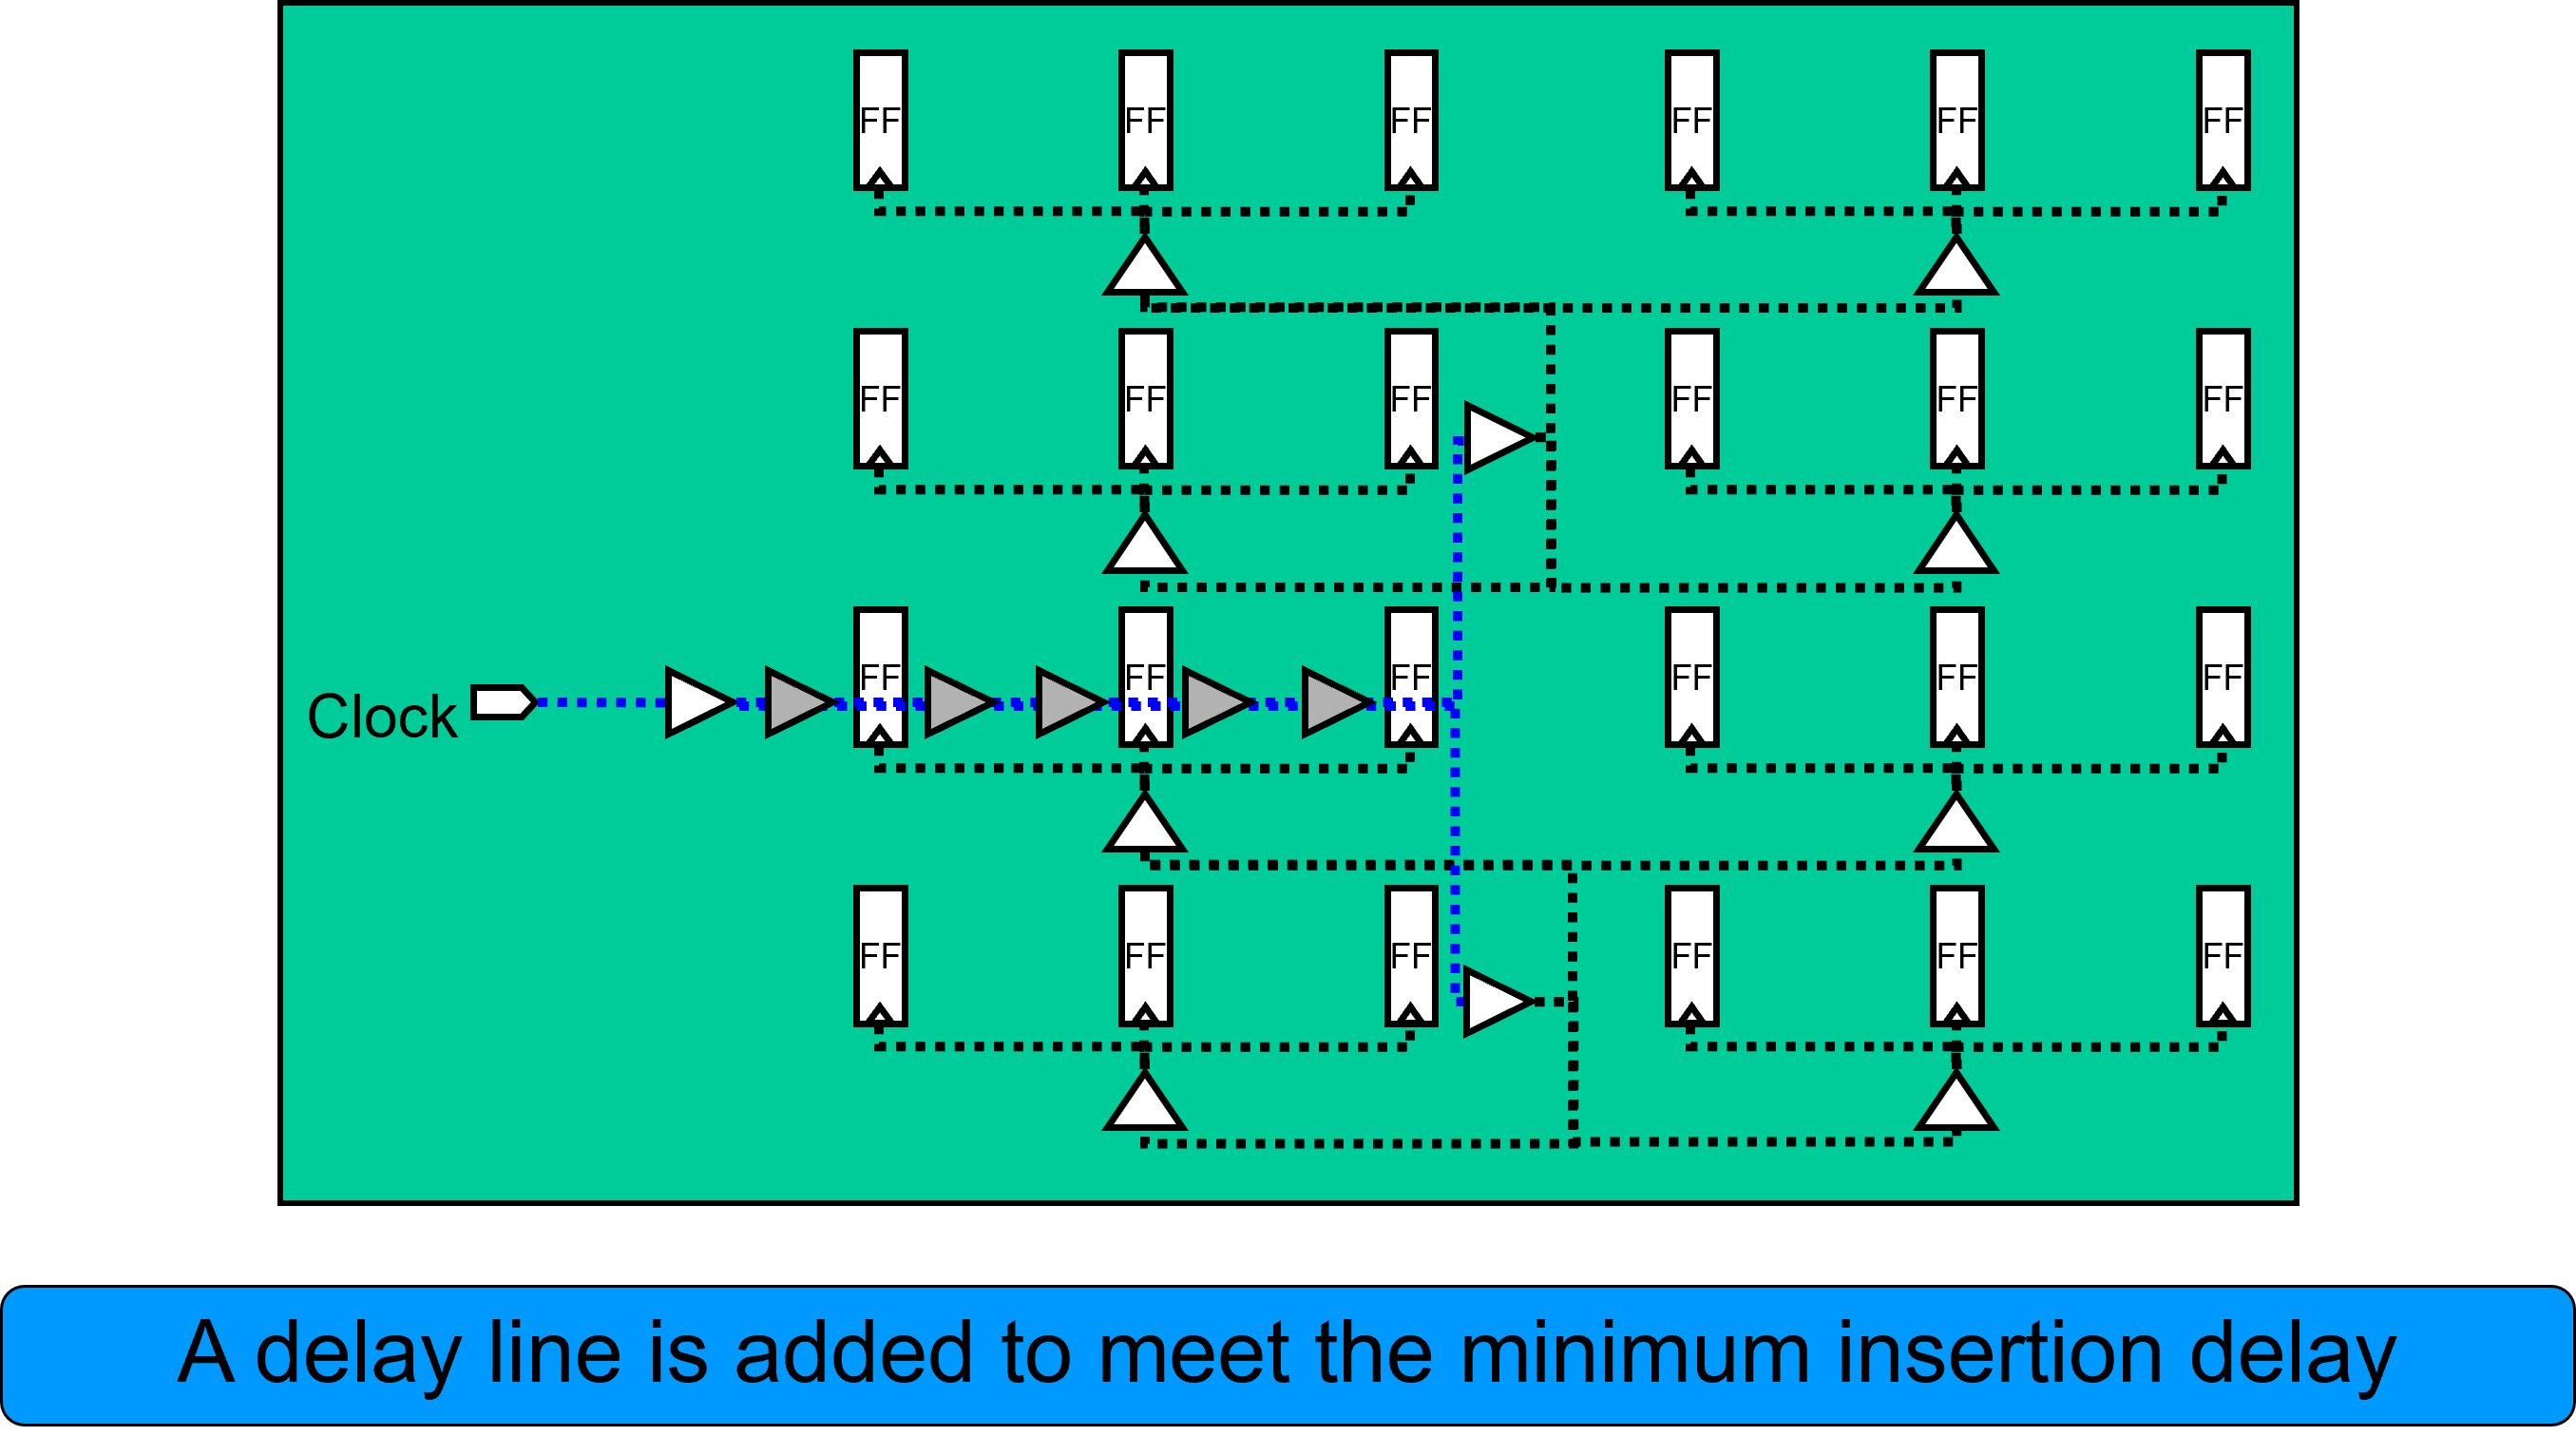
\includegraphics[width=\textwidth]{CTS3}
	\end{center}
\end{frame}
\subsection[Balance]{Balance}
\begin{frame}
	\frametitle{Clock Tree: General Concepts: Clock Distribution Network}
	\begin{center}
		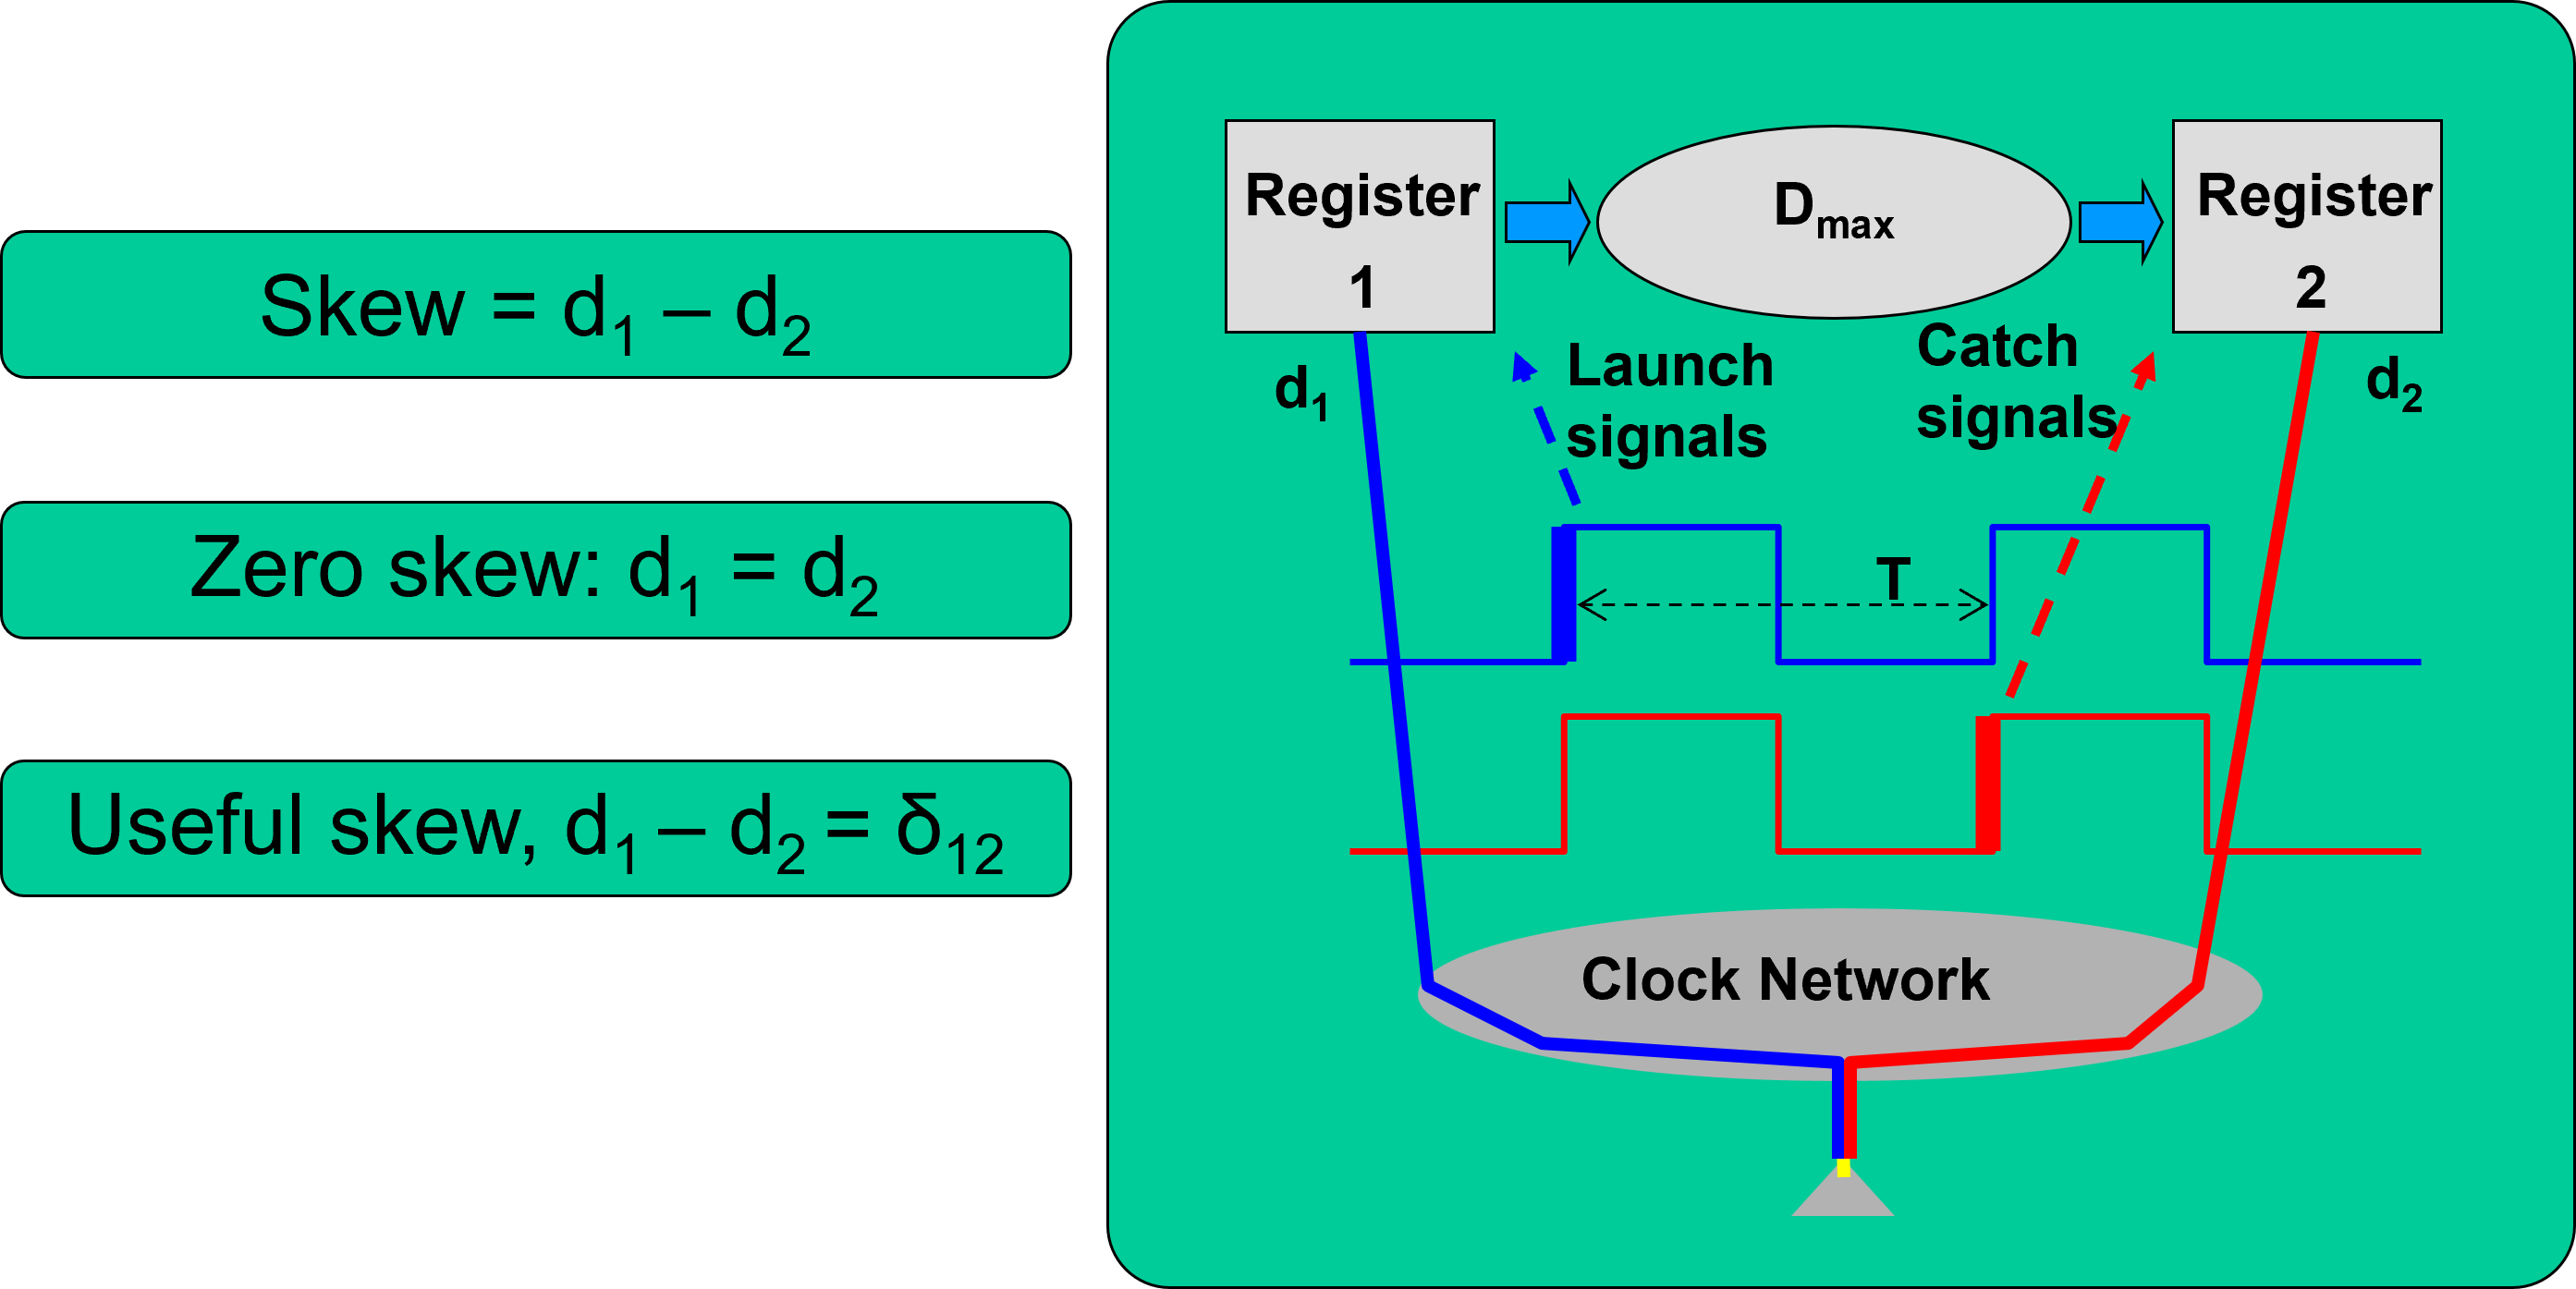
\includegraphics[width=\textwidth]{CTS4}
	\end{center}

\end{frame}

\begin{frame}
	\frametitle{Clock Tree: General Concepts: Clock Tree Goal and Metrics }
\begin{itemize}
	\item \textcolor{red}{\textbf{Goal}}
	\begin{itemize}
		\item Basic connectivity
	\end{itemize}
	
	\item \textcolor{red}{\textbf{Metrics}}
	\begin{itemize}
		\item Skew
		\item Power
		\item Area
		\item Slew rates
		
	\end{itemize}
	
\end{itemize}
\end{frame}
\begin{frame}
	\frametitle{Clock Tree: General Concepts: Clock Skew: Definition, Causes and Effects}
	\begin{center}
		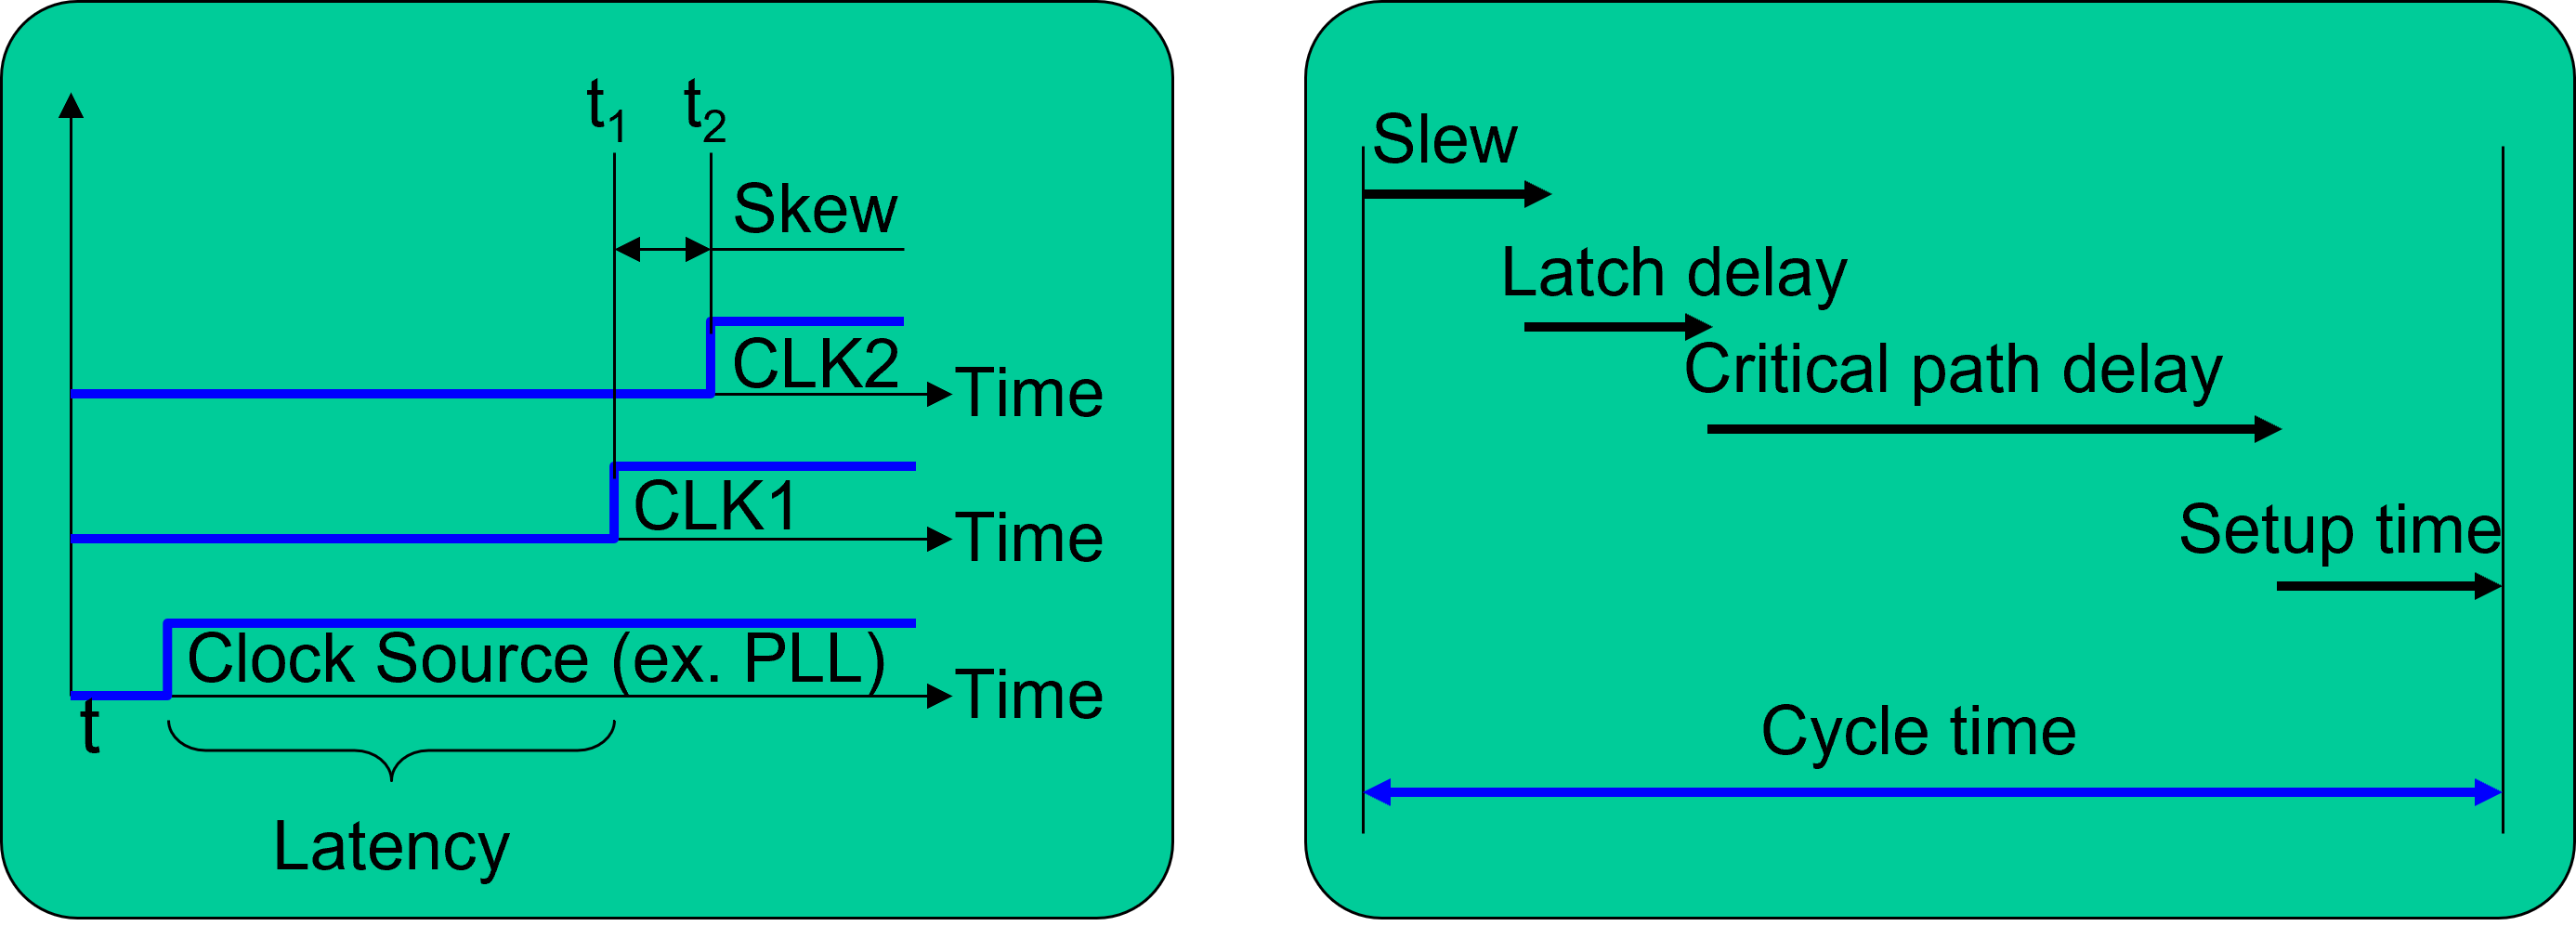
\includegraphics[width=\textwidth]{skew}
	\end{center}
\end{frame}
\subsection[Skew]{skew}
\begin{frame}
	\frametitle{Clock Skew Types}
	\begin{itemize}
		\item \textcolor{red}{\textbf{Global}}
		\begin{itemize}
			\item Global skew is recommended - fastest 
			\item may add unnecessary buffers
		\end{itemize}
		\item \textcolor{red}{\textbf{Local}}
		\begin{itemize}
			\item Longer runtime
			\item Possibly fewer buffers " Only related FFs are
			balanced for skew "
		\end{itemize}
		\item \textcolor{red}{\textbf{Useful}}
		\begin{itemize}
			\item Used to fix small violations where local or global failed
		\end{itemize}
		
	\end{itemize}
\end{frame}
\begin{frame}
	\frametitle{Global Skew: Fastest Runtime}
	\begin{center}
		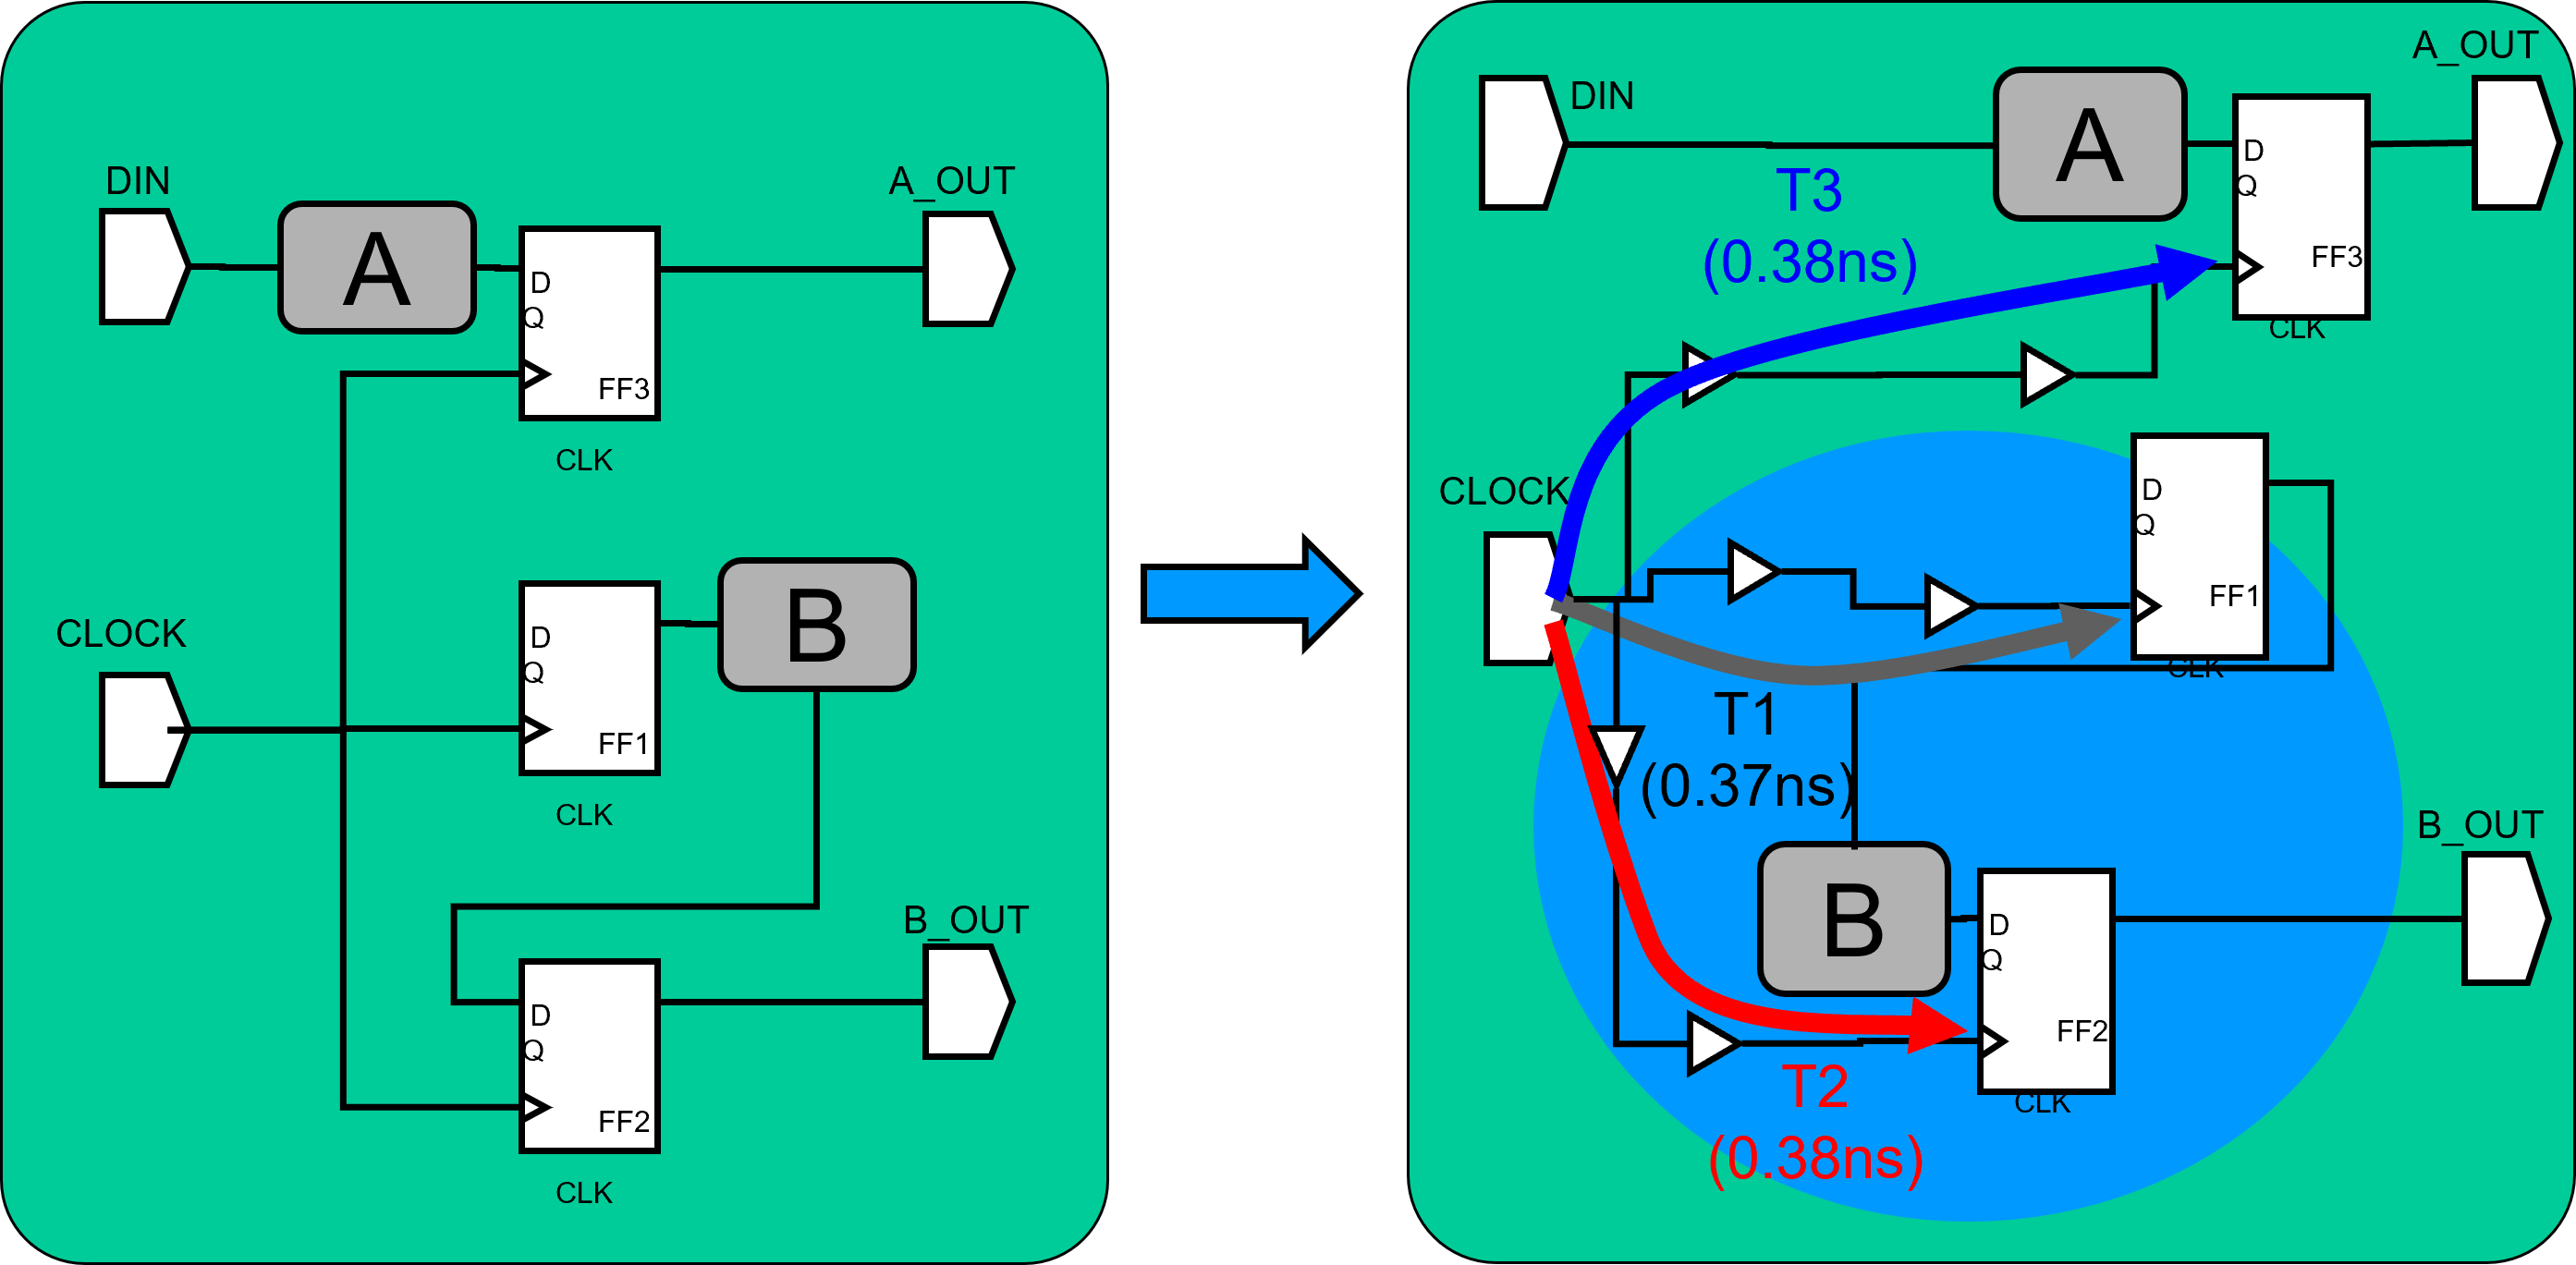
\includegraphics[width=\textwidth]{Global}
	\end{center}
\end{frame}
\begin{frame}
	\frametitle{Local Skew: Targeted Synthesis, But Slower}
		\begin{center}
		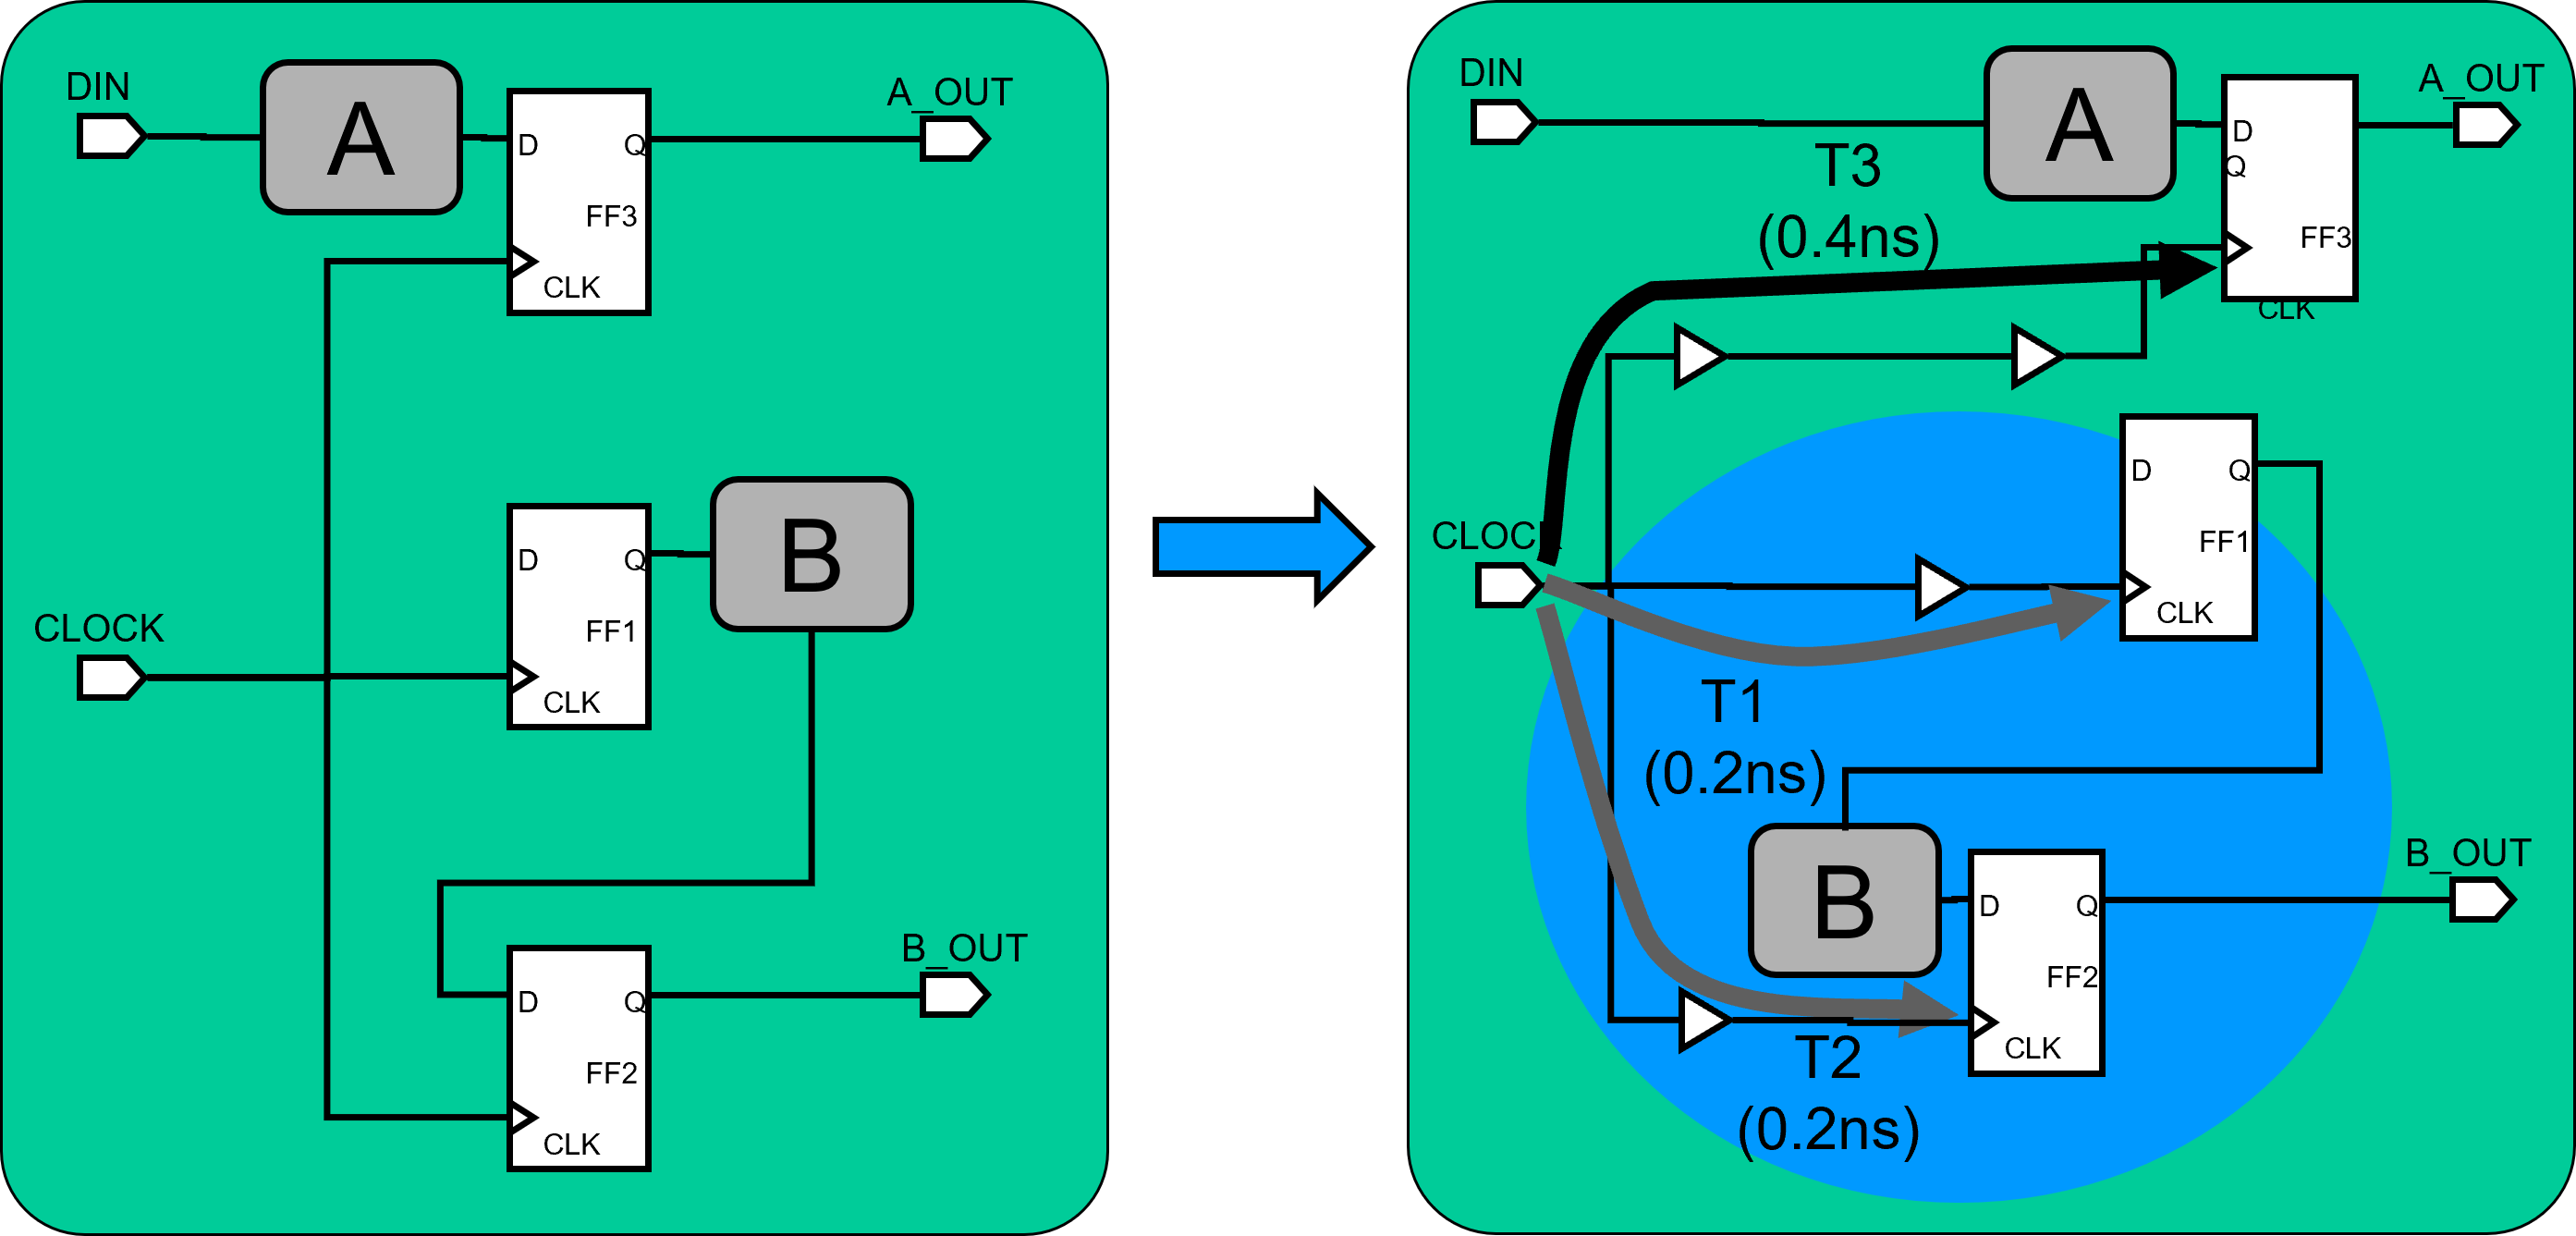
\includegraphics[width=\textwidth]{Local}
	\end{center}
\end{frame}
\begin{frame}
	\frametitle{Useful Skew}
		\begin{center}
		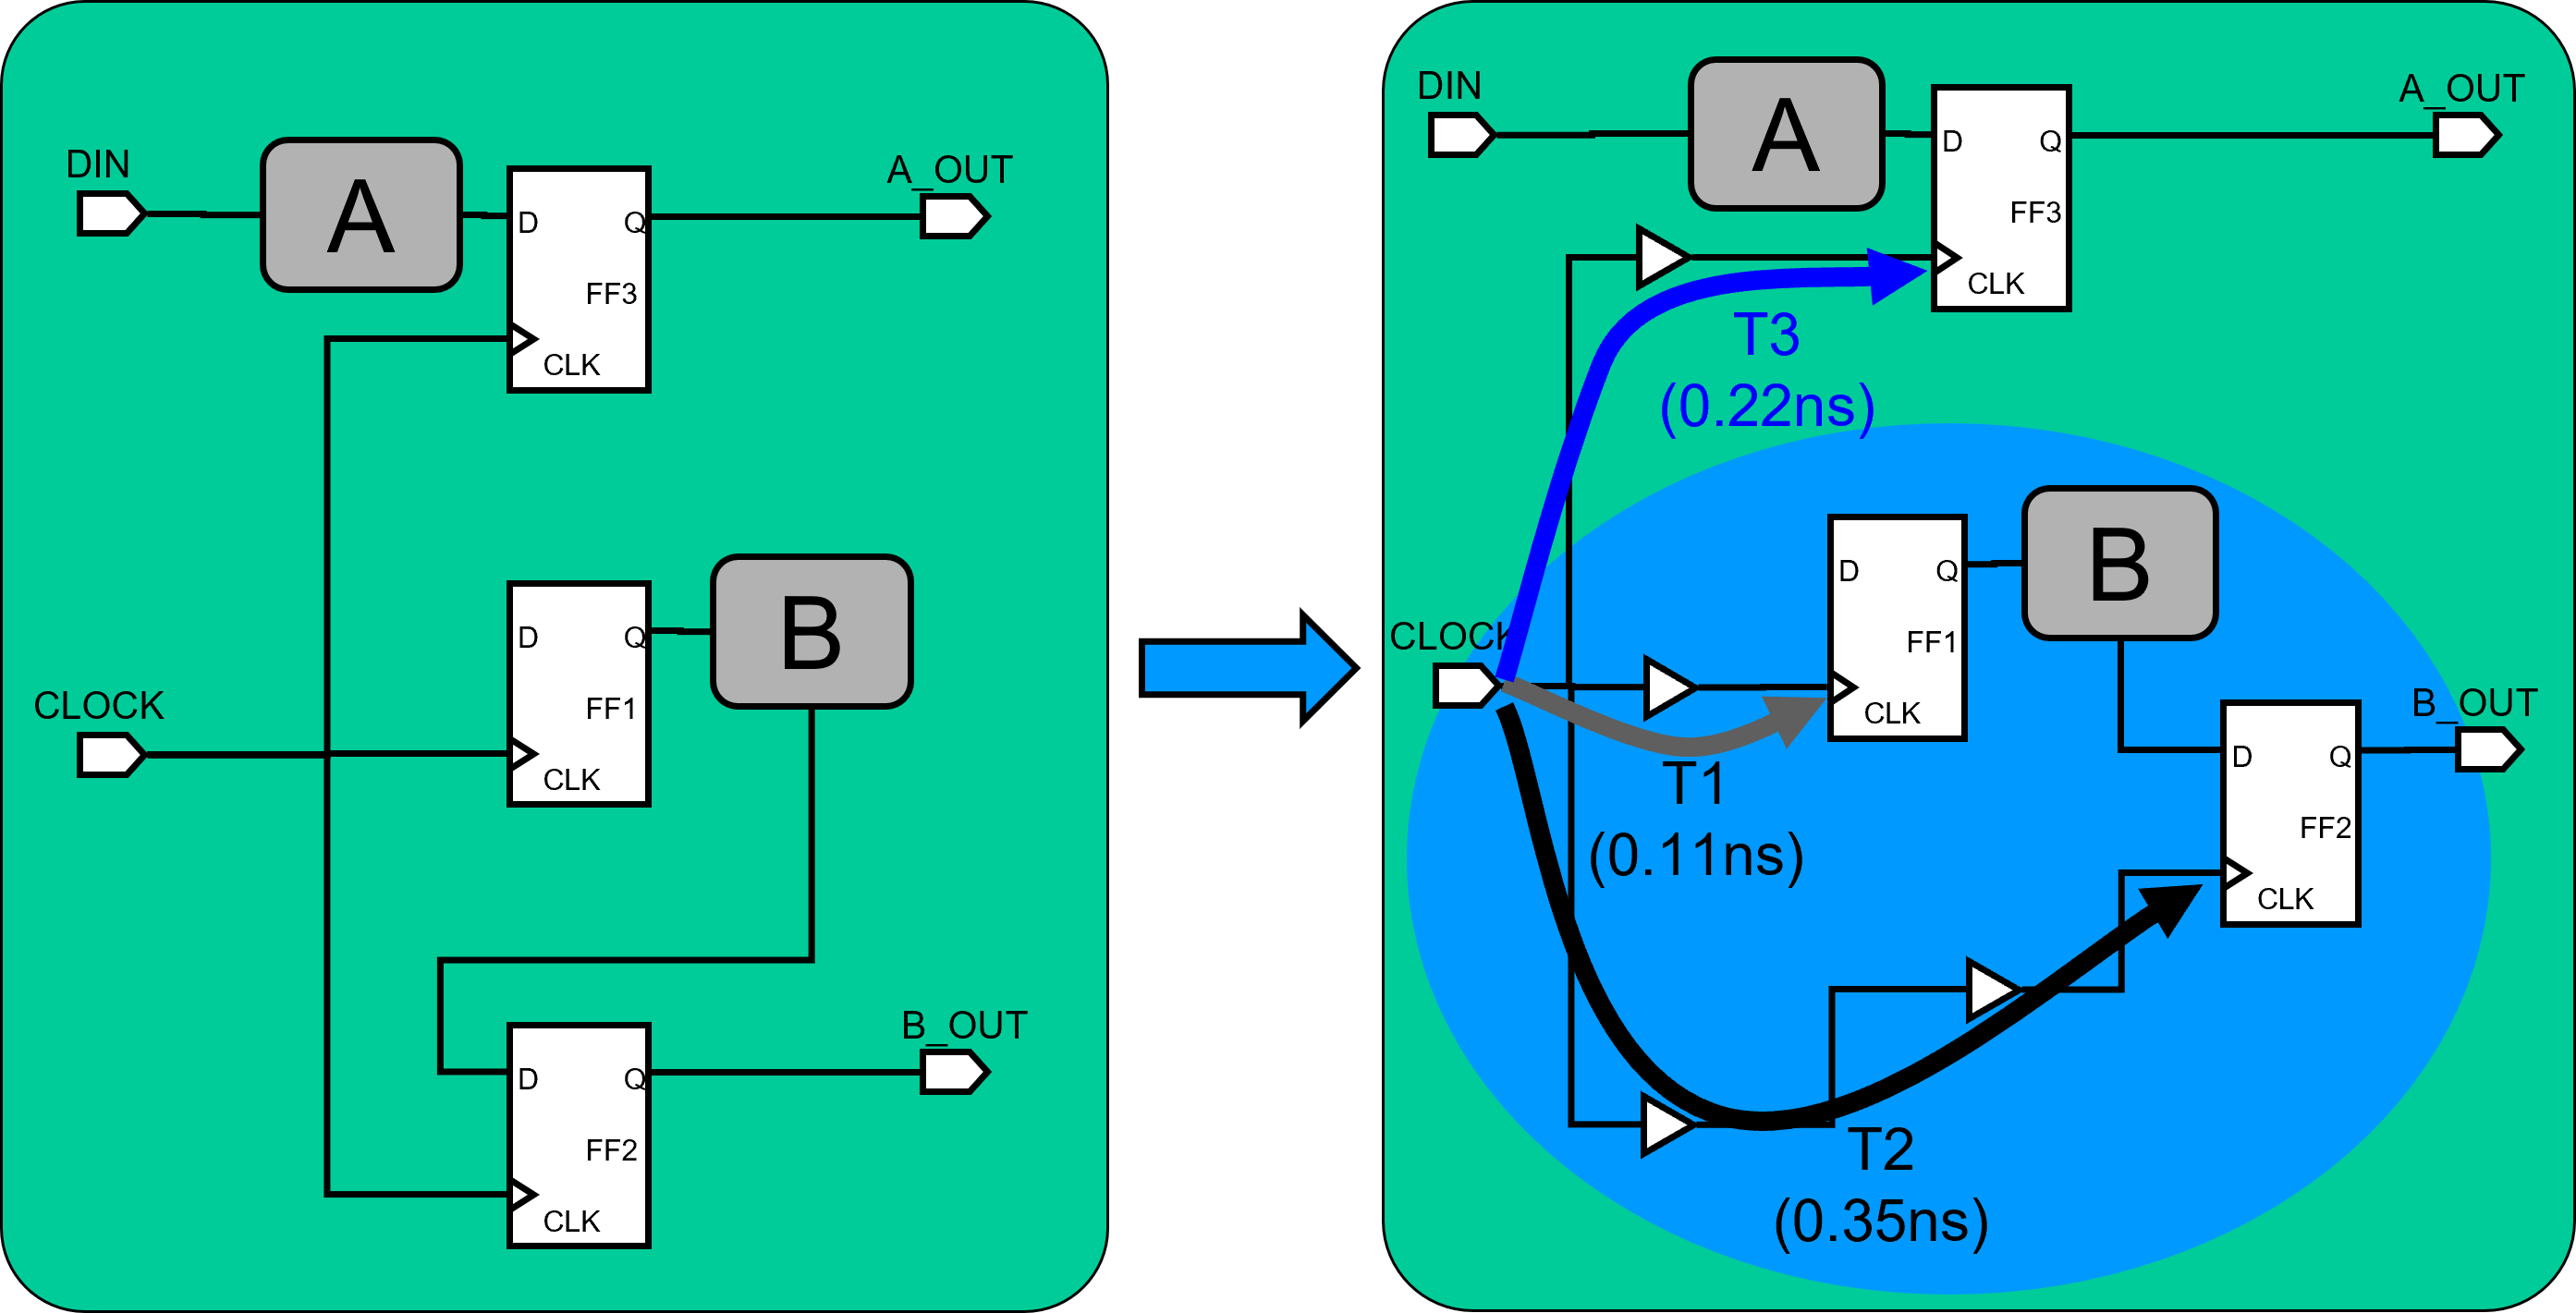
\includegraphics[width=\textwidth]{Useful}
	\end{center}

\end{frame}
%-------------------------------------------------
\section[CTS]{Clock Tree Synthesis}
\subsection[CTS]{Clock Tree Synthesis}
\begin{frame}
	\frametitle{Clock Tree Synthesis}
	\begin{center}
		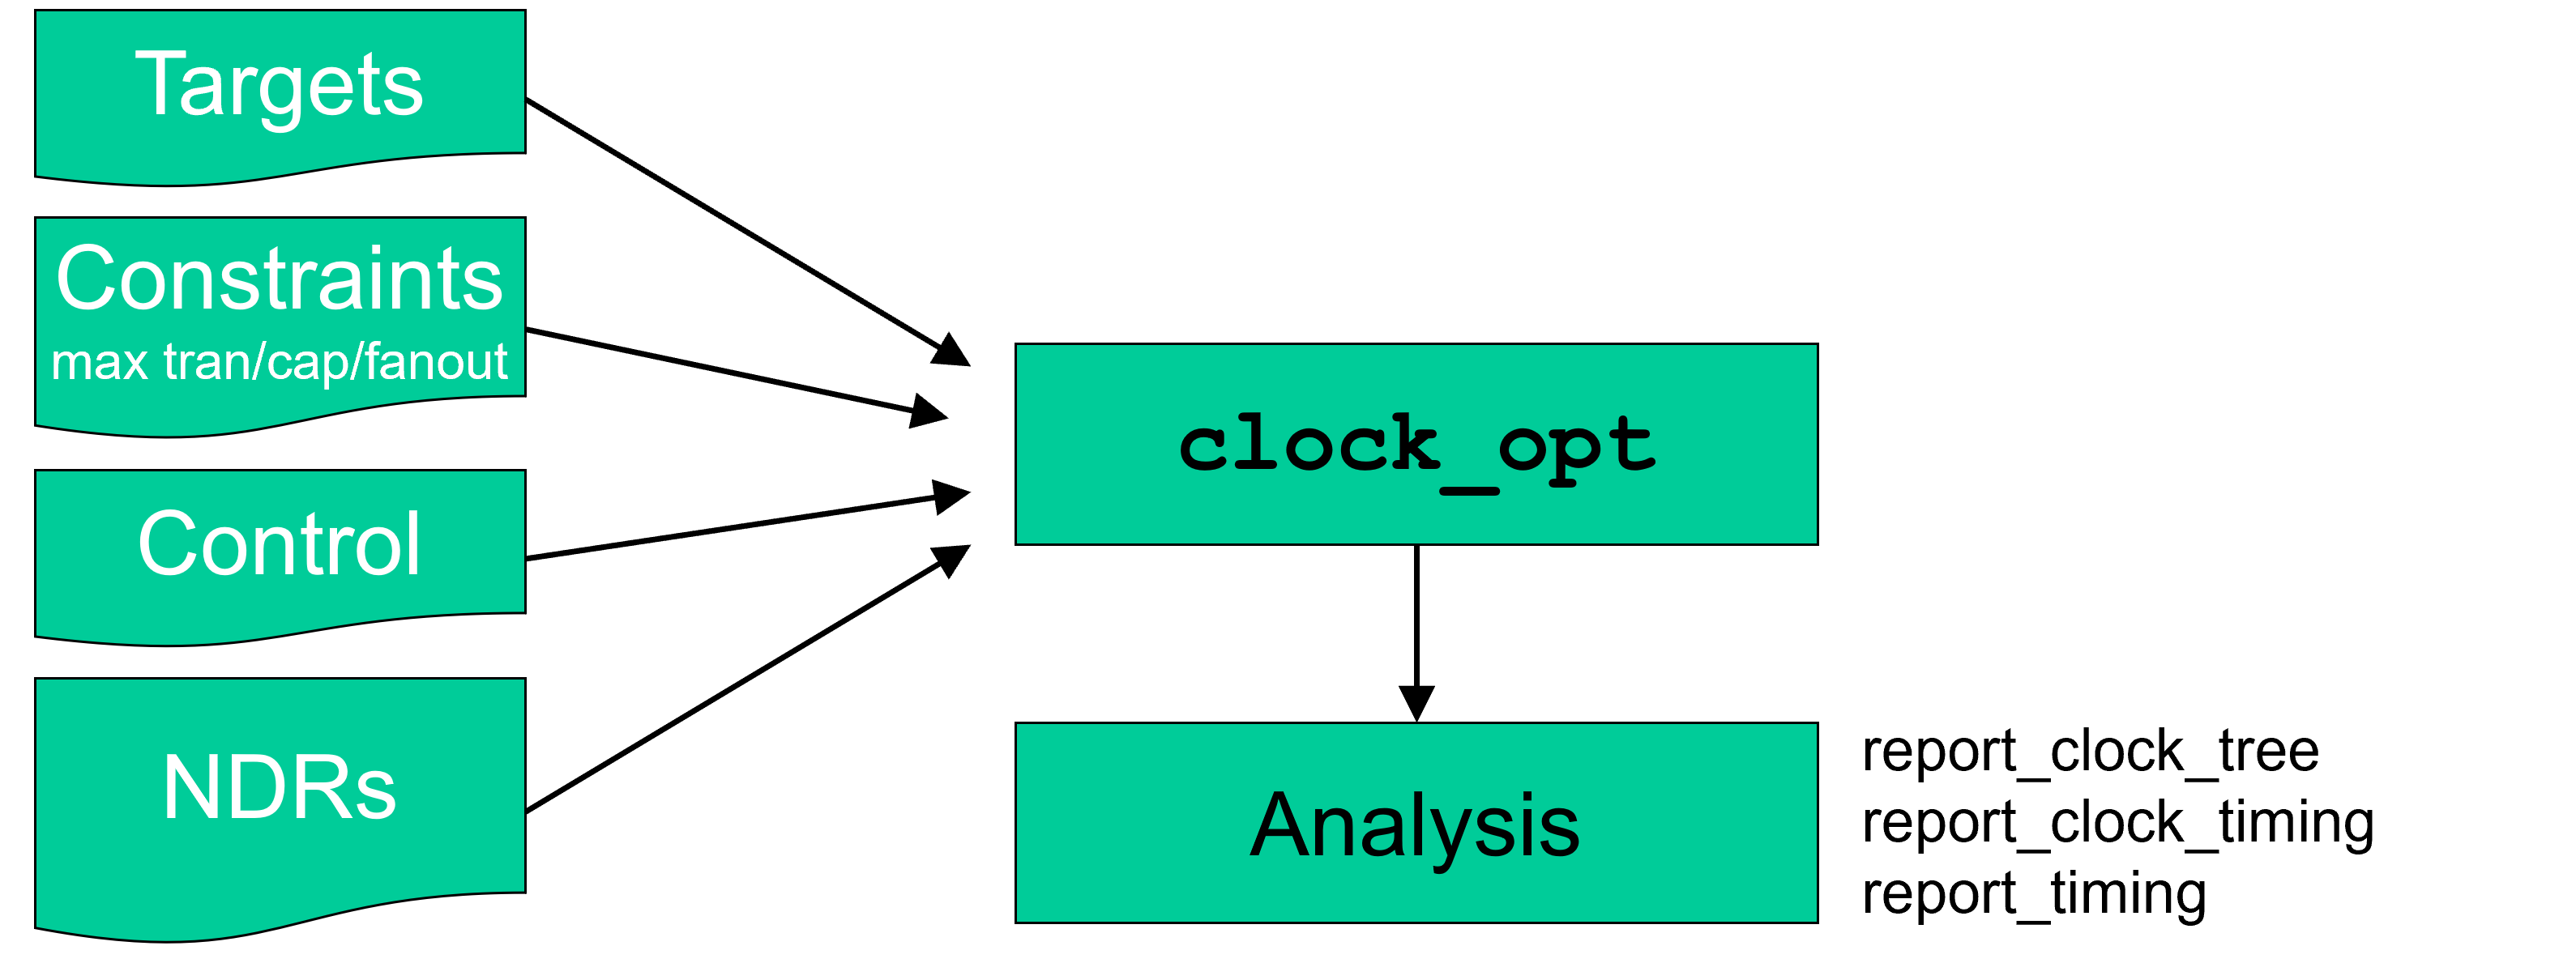
\includegraphics[width=\textwidth]{CTS0}
	\end{center}
\end{frame}

\begin{frame}
	\frametitle{Clock Tree Synthesis}
	\begin{center}
		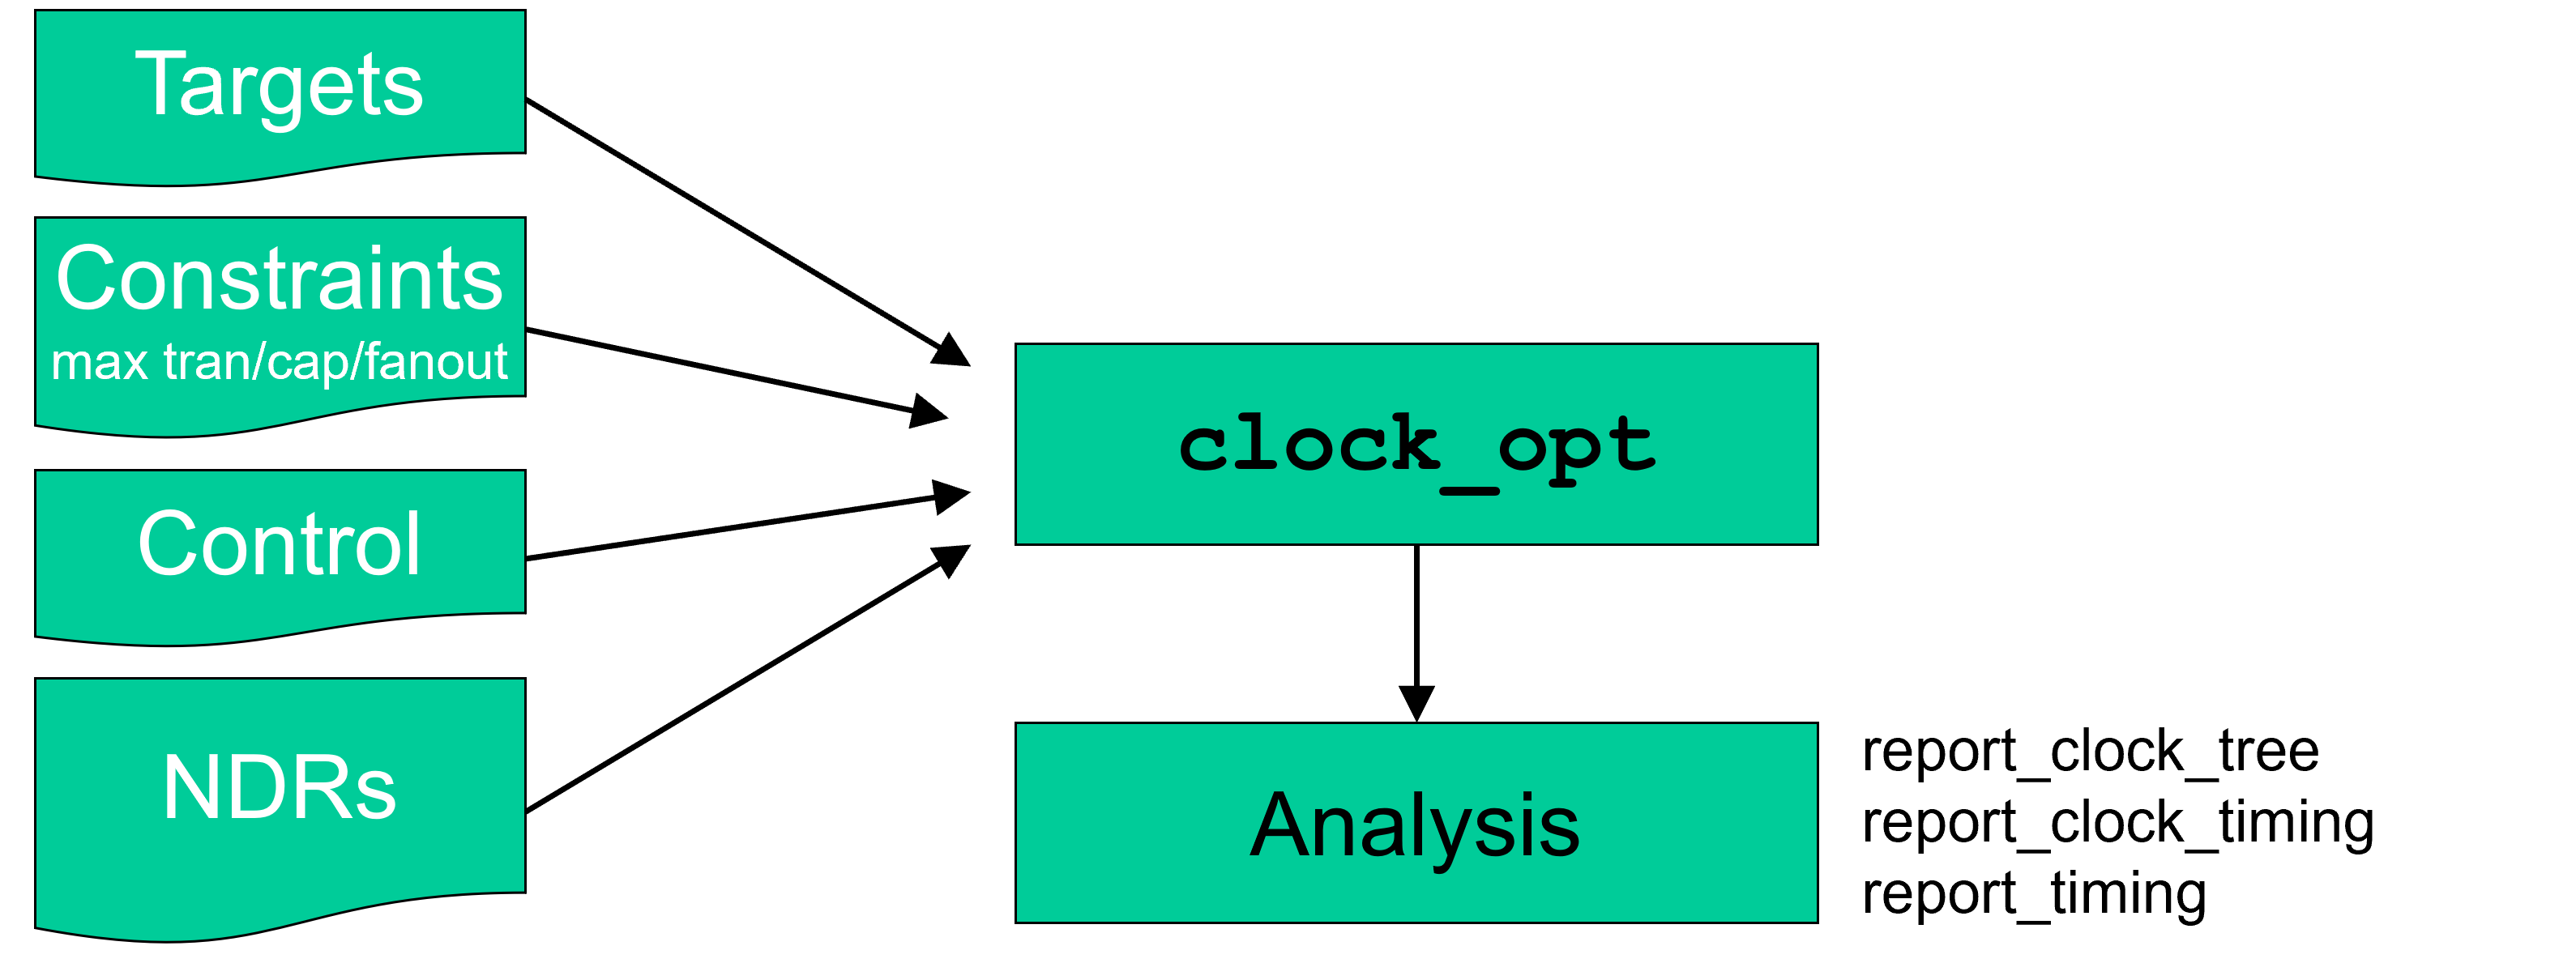
\includegraphics[width=\textwidth]{CTS0}
	\end{center}
\end{frame}
\subsection[Targets]{Targets}
\begin{frame}
	\frametitle{Understand Your Clock Tree Goals}
	\begin{itemize}
		\item \textbf{Skew Goal}
		\begin{itemize}
			\item \textcolor{red}{What are the skew requirements for your design?}
			\item \textcolor{red}{Are there different skew targets for small and large clocks?}
		\end{itemize}
		\item \textbf{Insertion Delay Goal}
		\begin{itemize}
			\item \textcolor{red}{What are the insertion delay specs for your block?}
			\item \textcolor{red}{What is a reasonable target based on the size and floorplan
				of your block/chip?}
		\end{itemize}
		\item \textbf{Nondefault rules to prevent SI problems}
		\item \textbf{DRC Requirements}
		\begin{itemize}
			\item \textcolor{red}{Are signal net DRCs different from clock net DRCs?}
		\end{itemize}
		\item \textbf{Find out the order of significance or importance of all the clocks in the design}
	\end{itemize}
\end{frame}
\begin{frame}
	\frametitle{Default Clock Tree Targets}
	\begin{itemize}
		\item \textbf{The default CTS target for skew and insertion
		delay is Ons}
		\begin{itemize}
			\item Uncertainty and insertion delay SDC constraints are	ignored
		\end{itemize}
		\item \textbf{It is recommended to relax the clock skew target
		as much as possible}
	\begin{itemize}
		\item  Reduces overall buffer count, Power, and run time
	\end{itemize}
		\item \textbf{Specify minimum clock latencies as needed}
	\end{itemize}
\end{frame}
\subsection[Cons]{Constraints}
\begin{frame}
	\frametitle{Constraints: Are all Clock Drivers and Loads Specified?}
	\begin{center}
		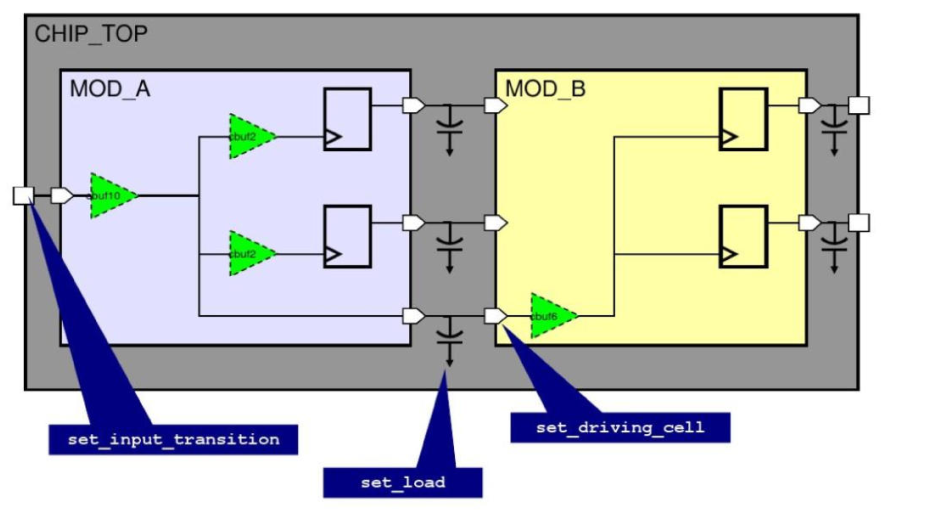
\includegraphics[width=\textwidth]{Constraints}
	\end{center}
\end{frame}

\subsection[Control]{Control}
\begin{frame}
	\frametitle{Where Does the Clock Tree Begin and End?}
	\begin{center}
		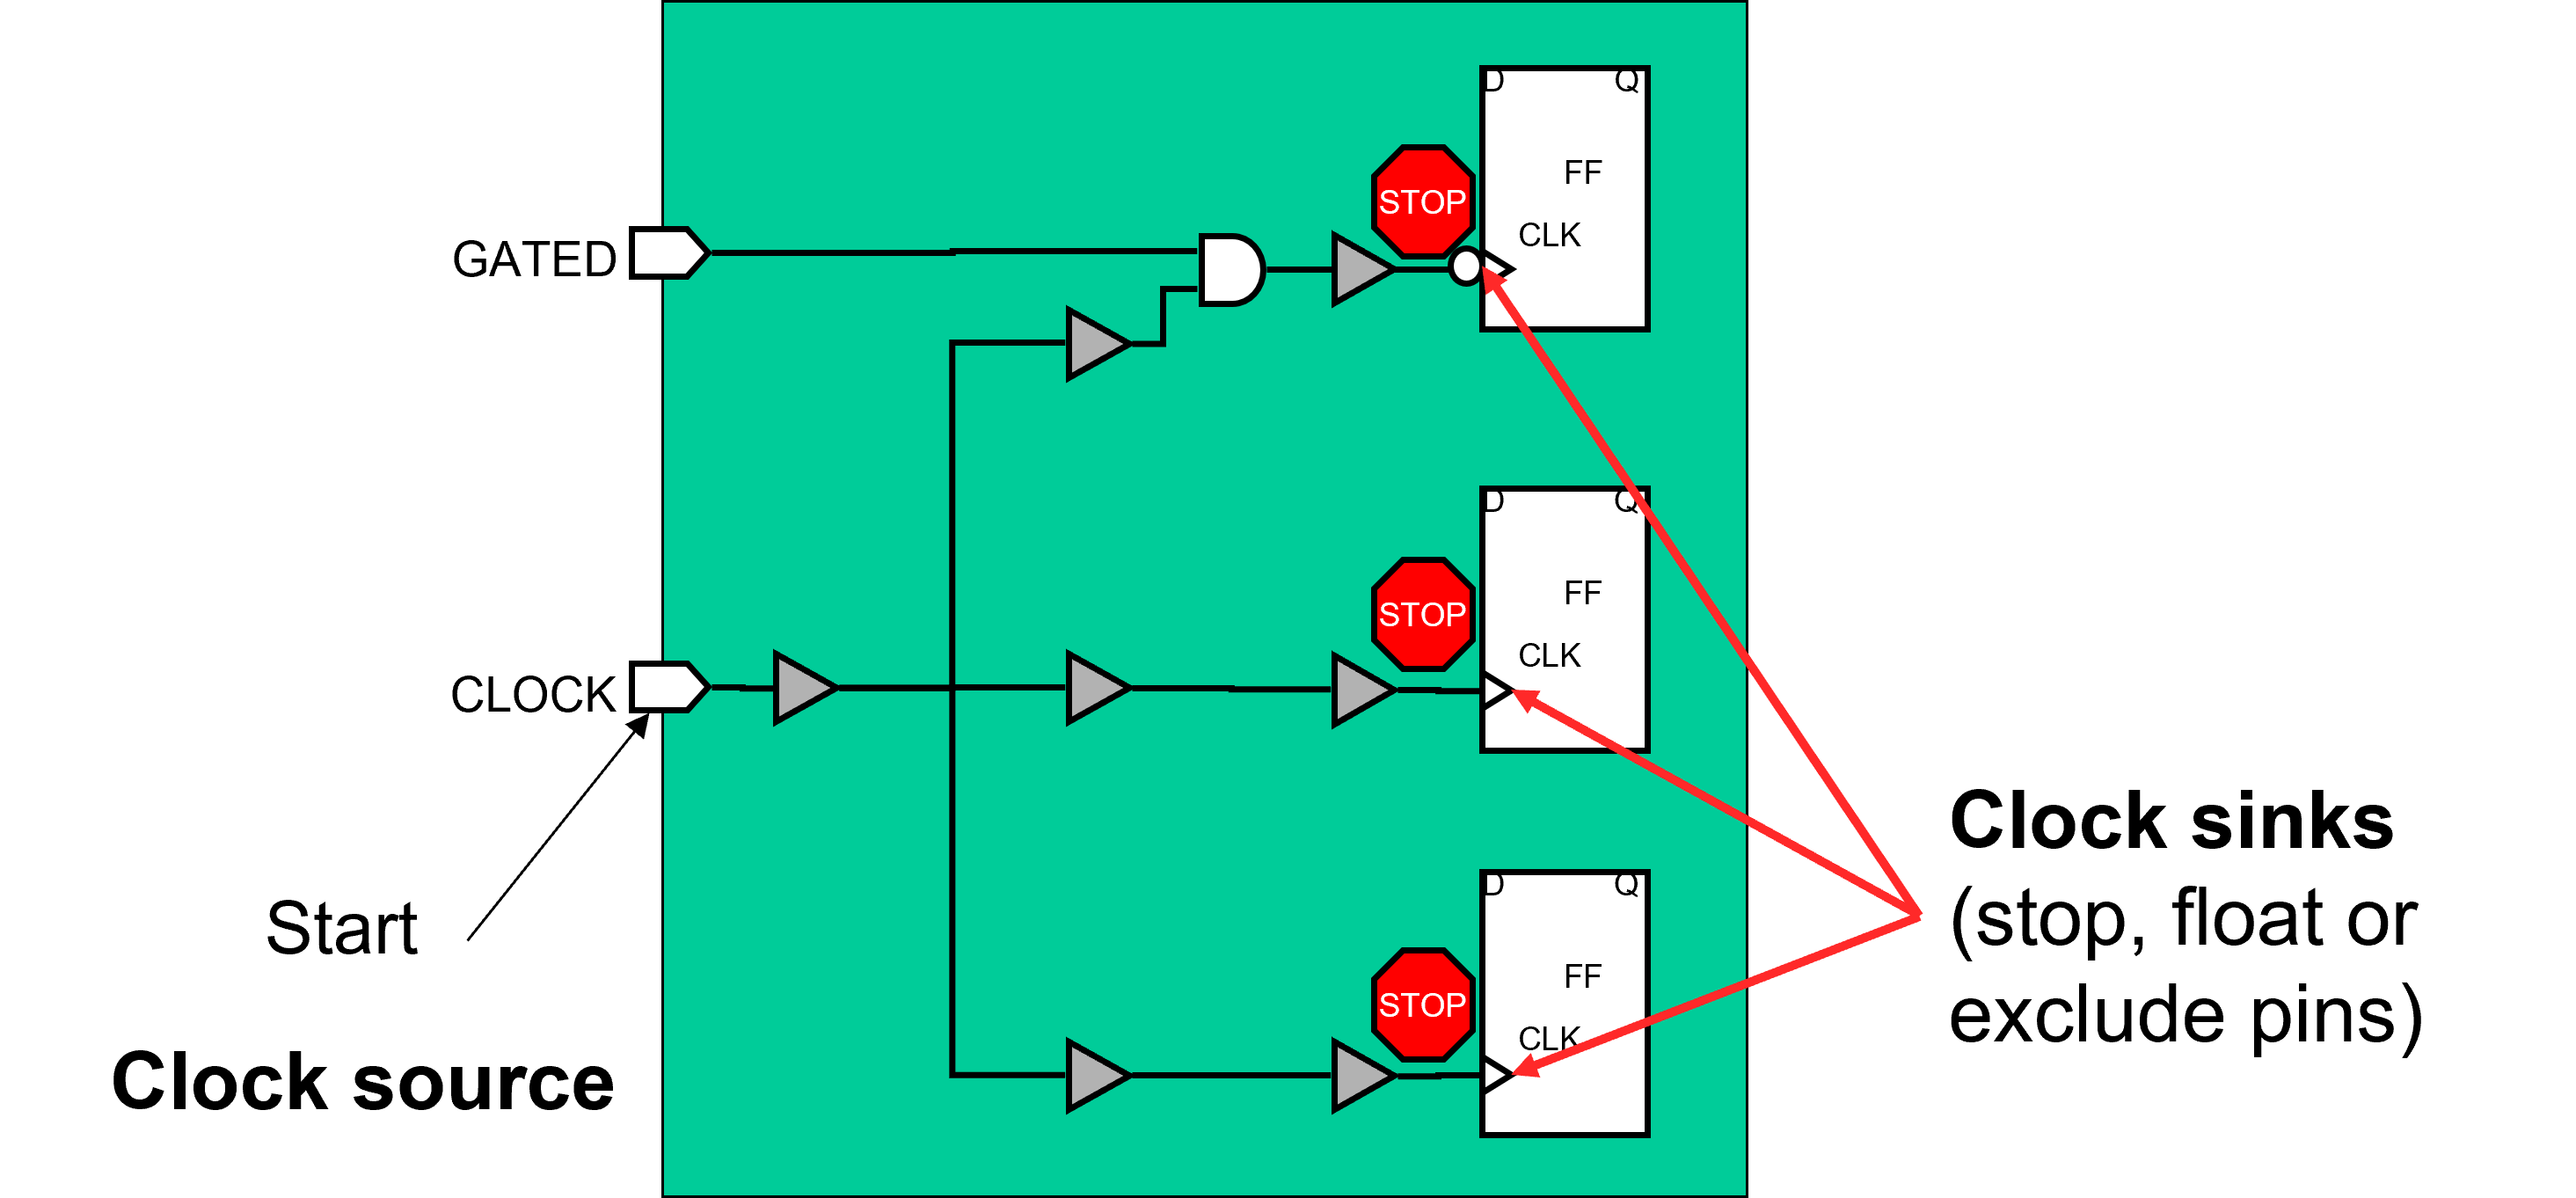
\includegraphics[width=\textwidth]{Start}
	\end{center}
\end{frame}

\begin{frame}
	\frametitle{Define Clock Root Attributes (1/2)}
	\begin{itemize}
		\item \textbf{When the clock root is a primary port of a block}
		\begin{itemize}
			\item Ensure that an appropriate driving cell is defined
			\textcolor{green}{set\_driving\_cell }
			\item The synthesis constraints may include a weak driving cell for all inputs, including the clock port
			\item Because the clock is ideal during synthesis it has no effect on design QoR
			\item But a weak driver on the clock port affects clock tree QoR during CTS
		\end{itemize}
	\end{itemize}
\begin{center}
	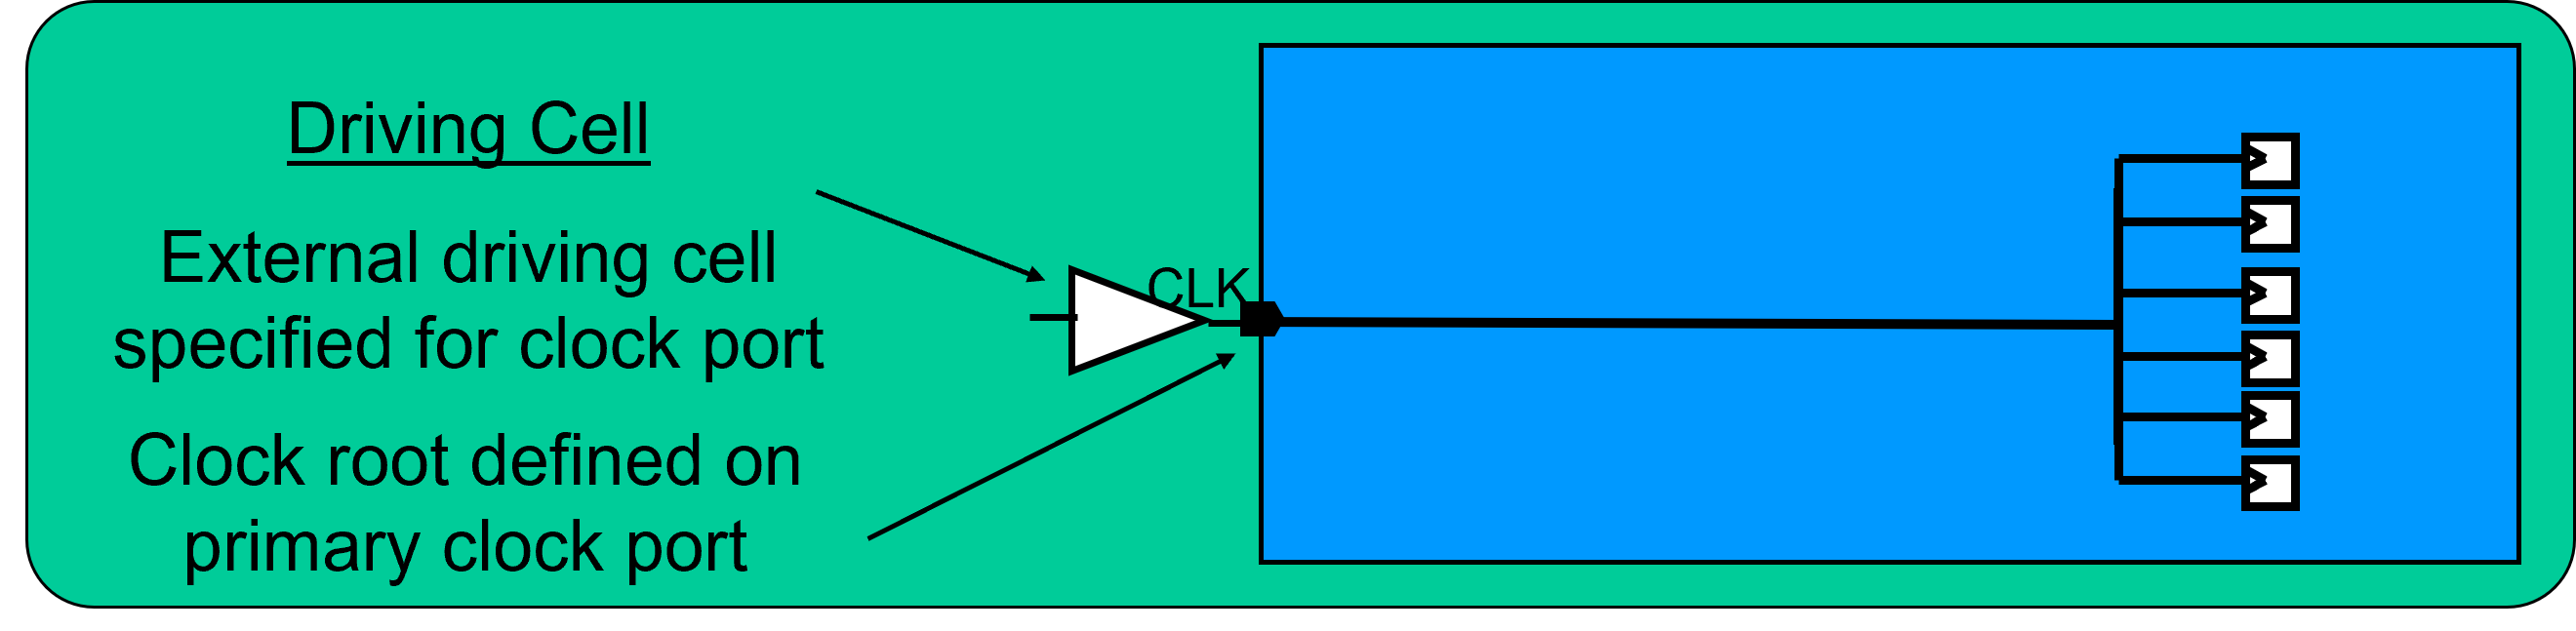
\includegraphics[width=0.7\textwidth]{root}
\end{center}
\end{frame}
\begin{frame}
	\frametitle{Define Clock Root Attributes (2/2)}
		\begin{itemize}
	\item \textbf{When the clock root is a primary port, but at the CHIP-level through an IO-PAD}
		\begin{itemize}
		\item Ensure that an appropriate input transition is defined
		
		\textcolor{green}{set\_input\_transition  }
	\end{itemize}
\end{itemize}
\begin{center}
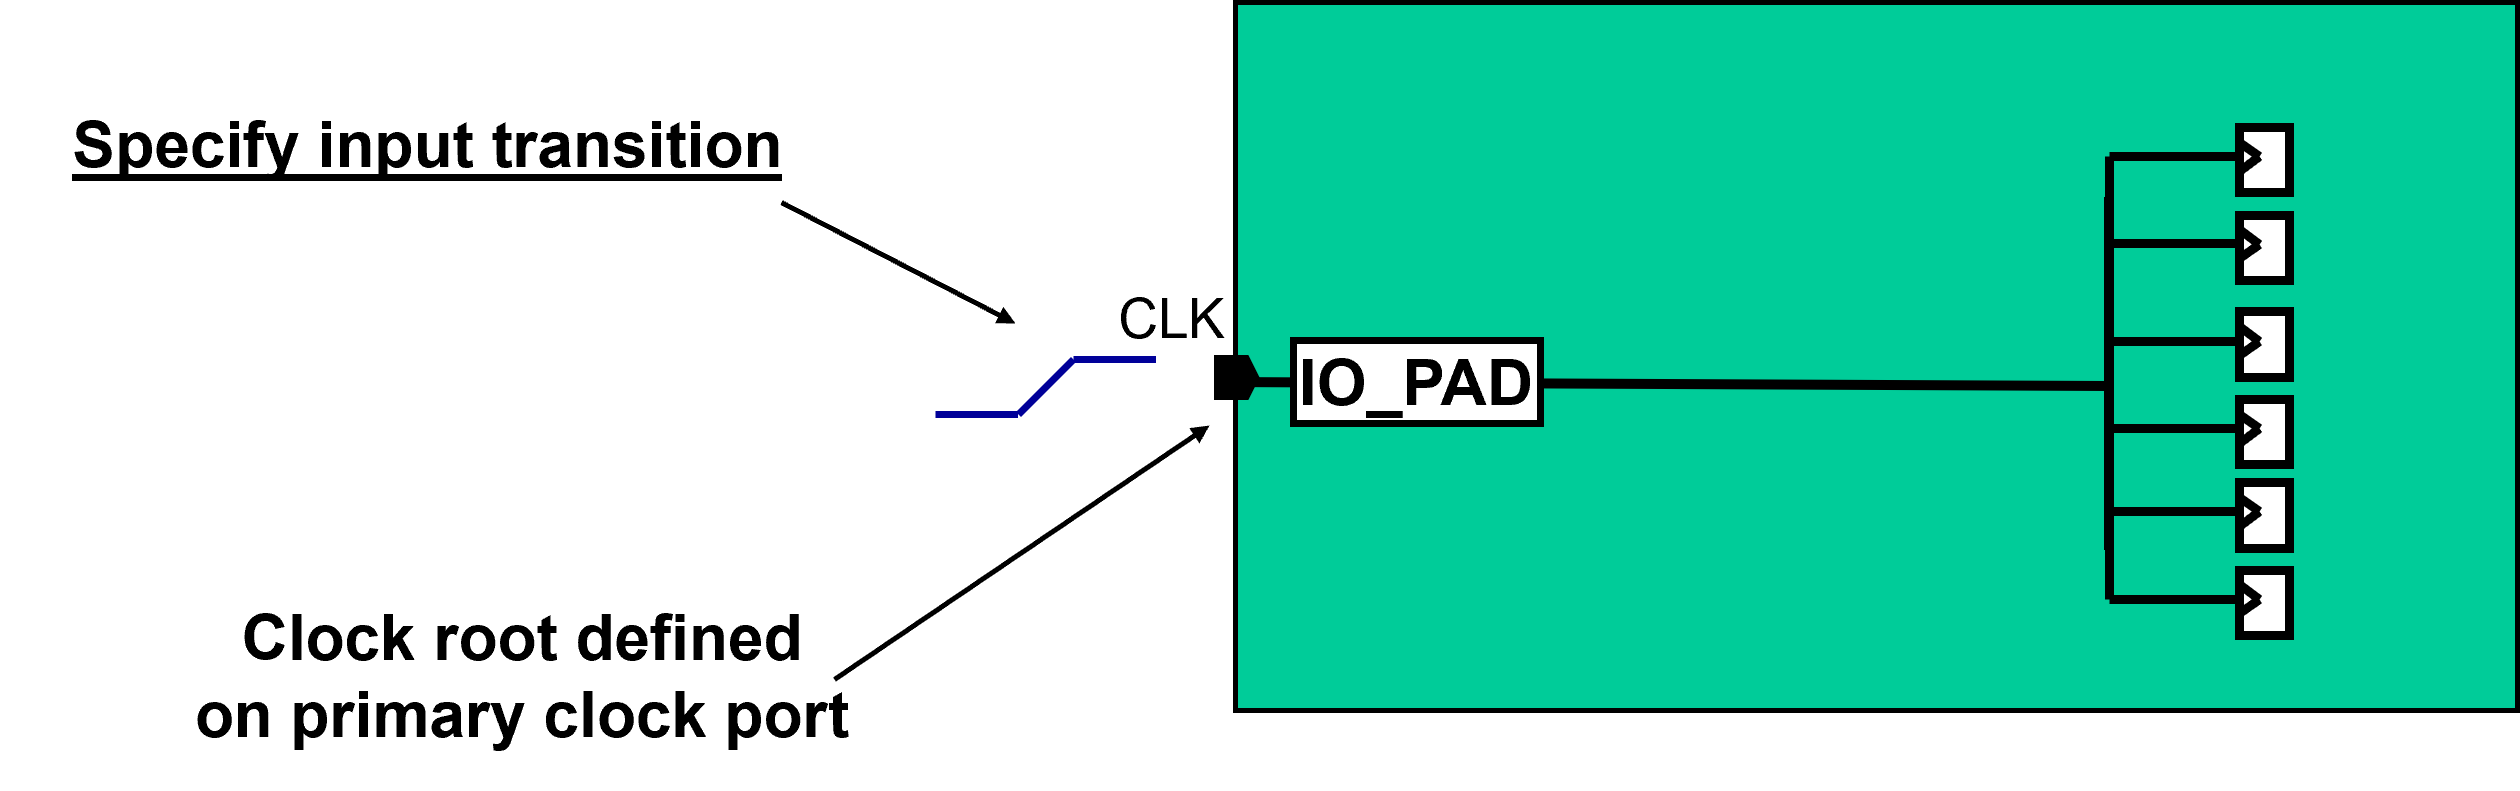
\includegraphics[width=0.9\textwidth]{IO-PAD}
\end{center}
\end{frame}

\begin{frame}
	\frametitle{Stop, Float and Exclude Pins}
	\begin{columns}	
		\column{0.6\textwidth}
		\begin{itemize}
			\item \textbf{Stop Pins:}
			\begin{itemize}
				\item CTS optimizes for DRC and clock tree targets (skew, insertion delay)
			\end{itemize}
		\item \textbf{Float Pins:}
			\begin{itemize}
				\item Like Stop pins, but with delays on clock pin
			\end{itemize}
		\item \textbf{Exclude (Ignore) Pins:}
		\begin{itemize}
			\item CTS ignores skew and
			insertion delay targets
			\item CTS will fix DRCs to meet library or SDC constraints
		\end{itemize}
		\end{itemize}
		\column{0.6\textwidth}
		\begin{center}
		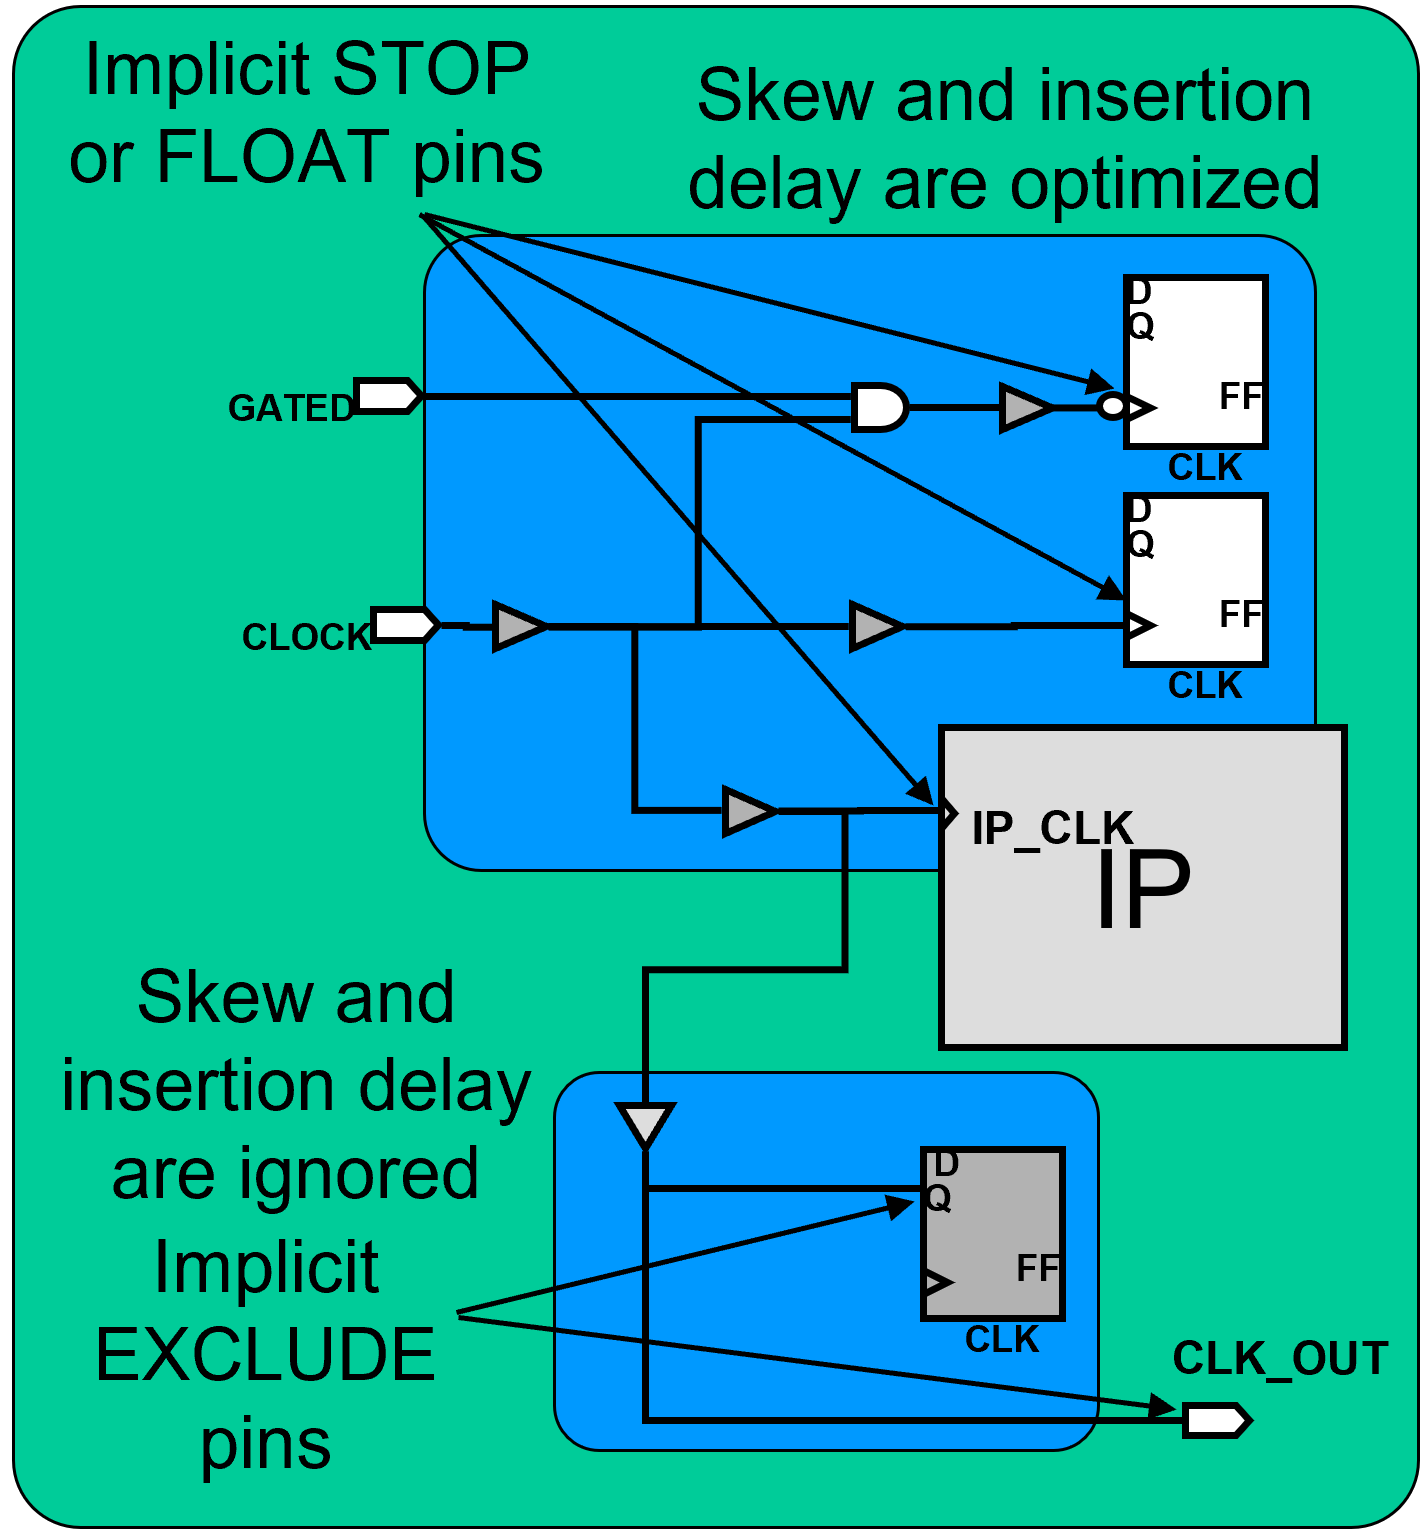
\includegraphics[width=0.8 \textwidth]{Exception}
	\end{center}
	\end{columns}
\end{frame}

\begin{frame}
	\frametitle{Generated and Gated Clocks}
	\begin{center}
		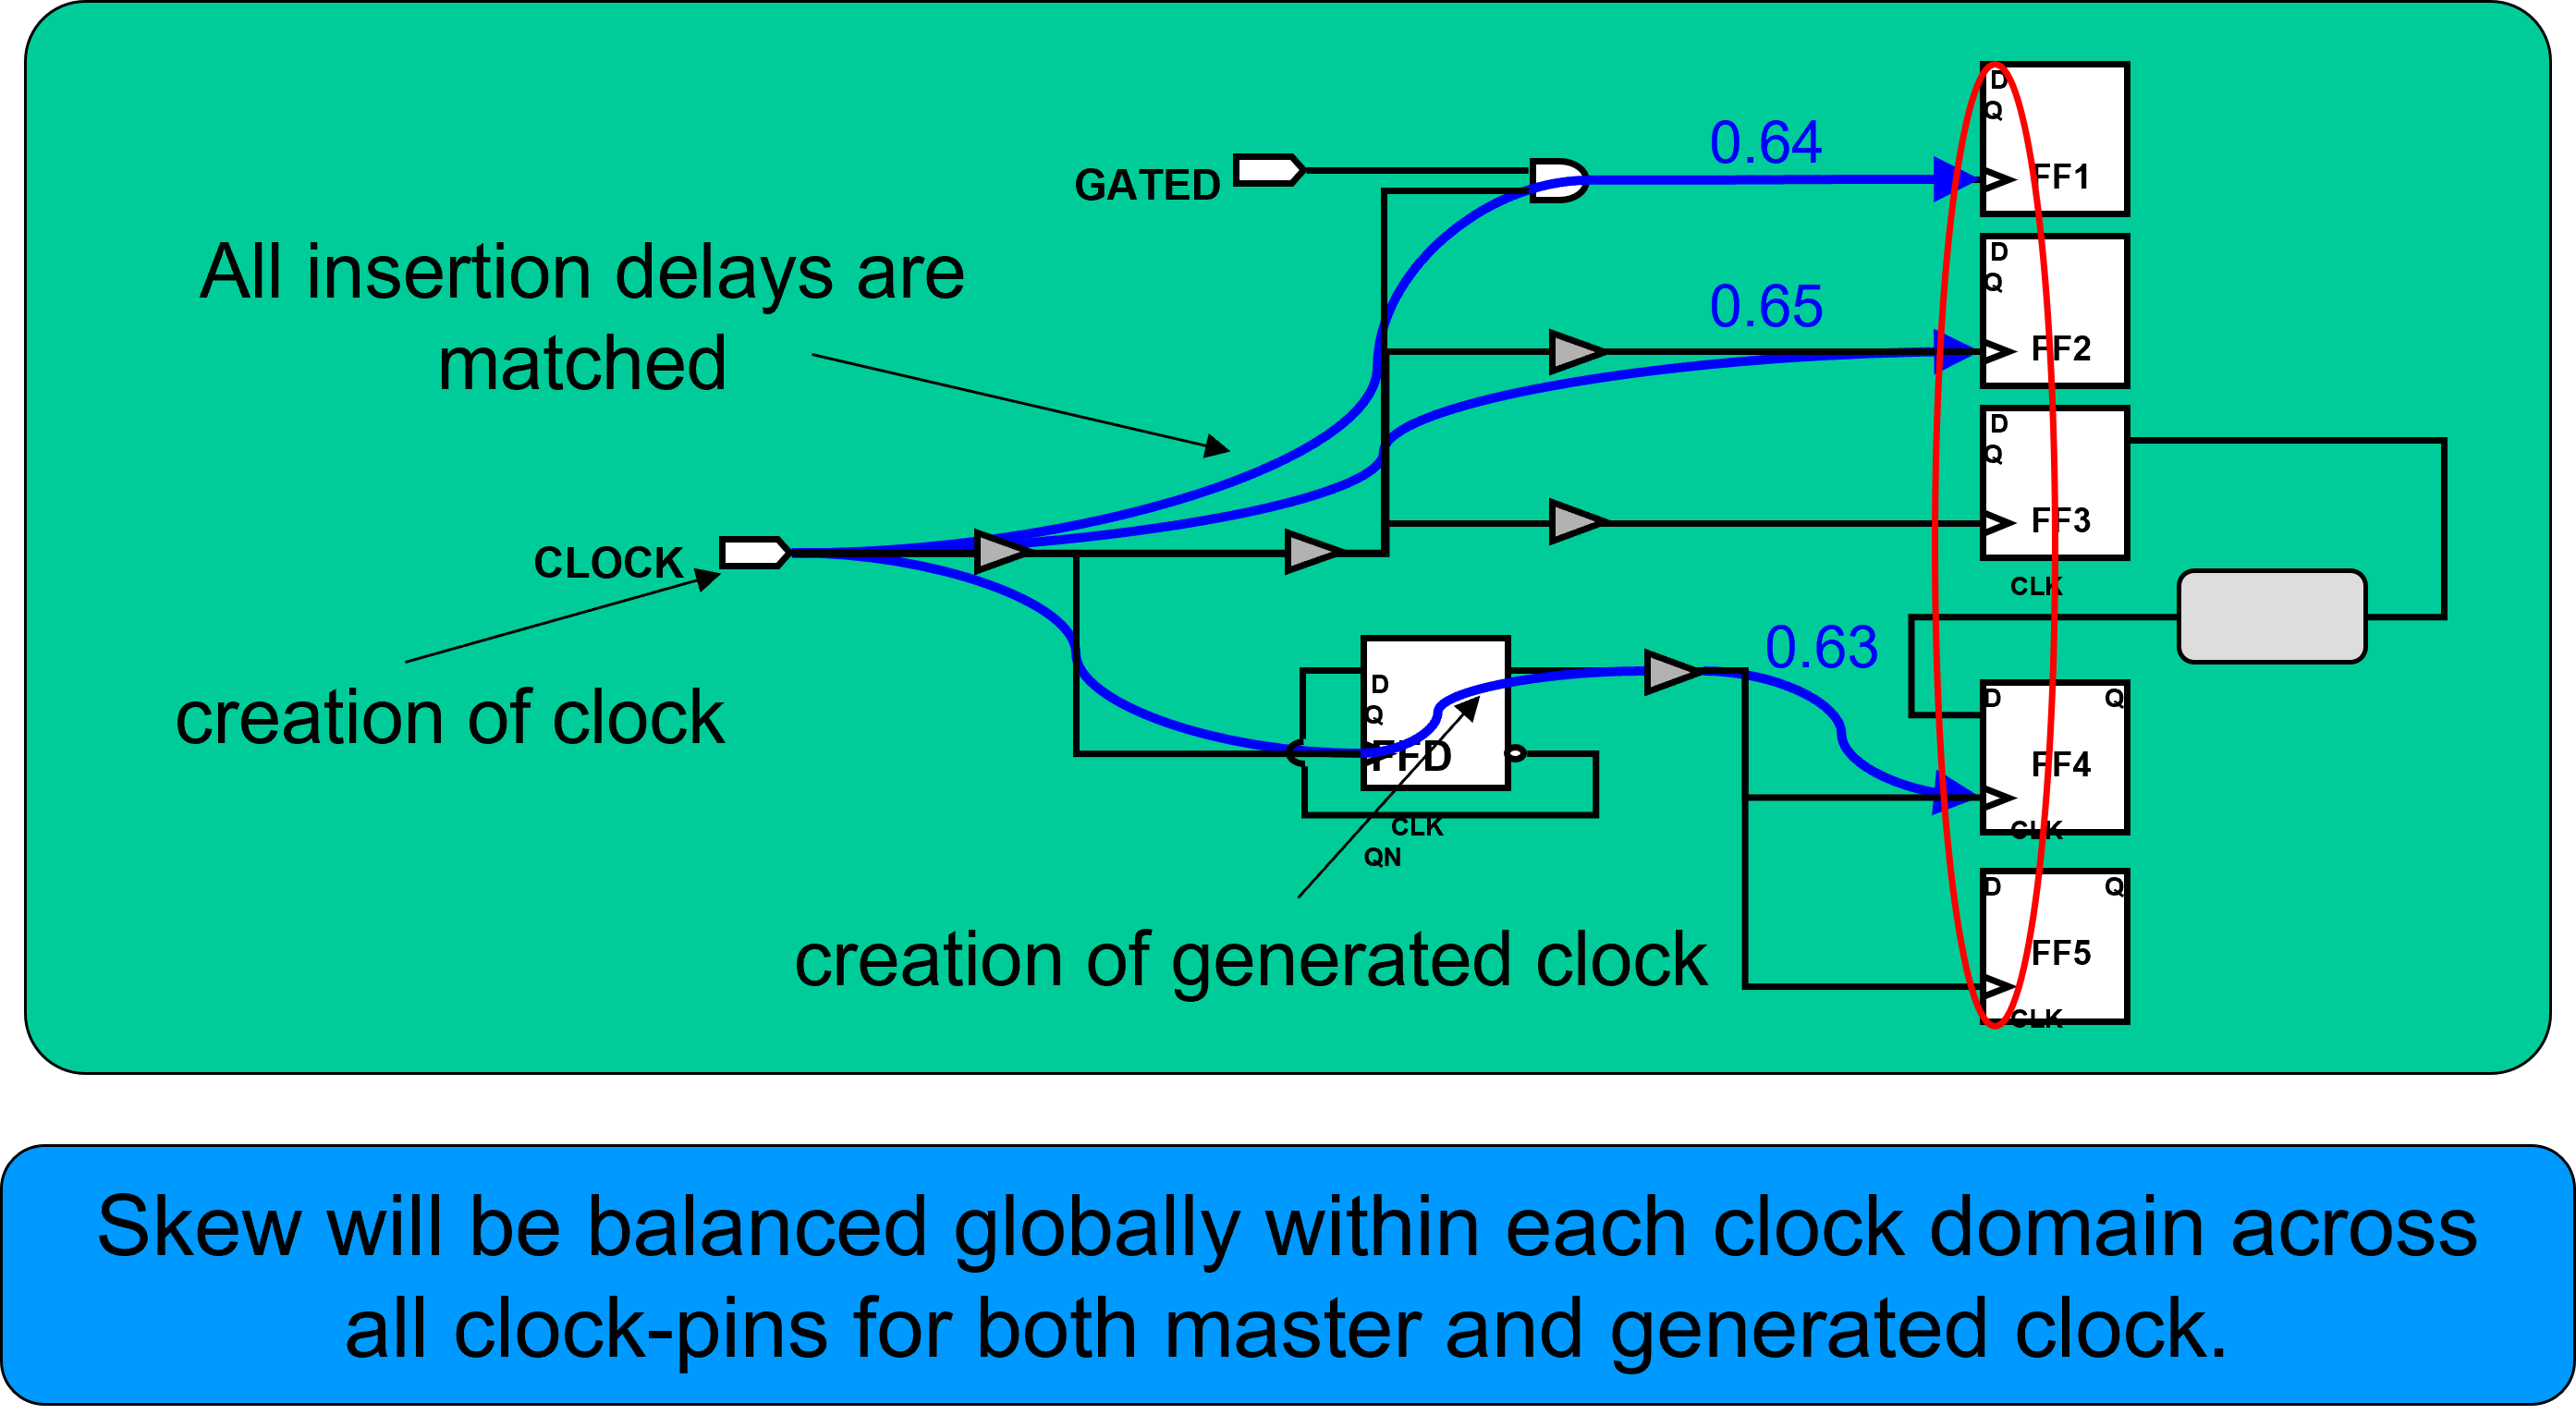
\includegraphics[width=\textwidth]{Generated}
	\end{center}
\end{frame}

\begin{frame}
	\frametitle{Skew Balancing not Required}
	\begin{center}
		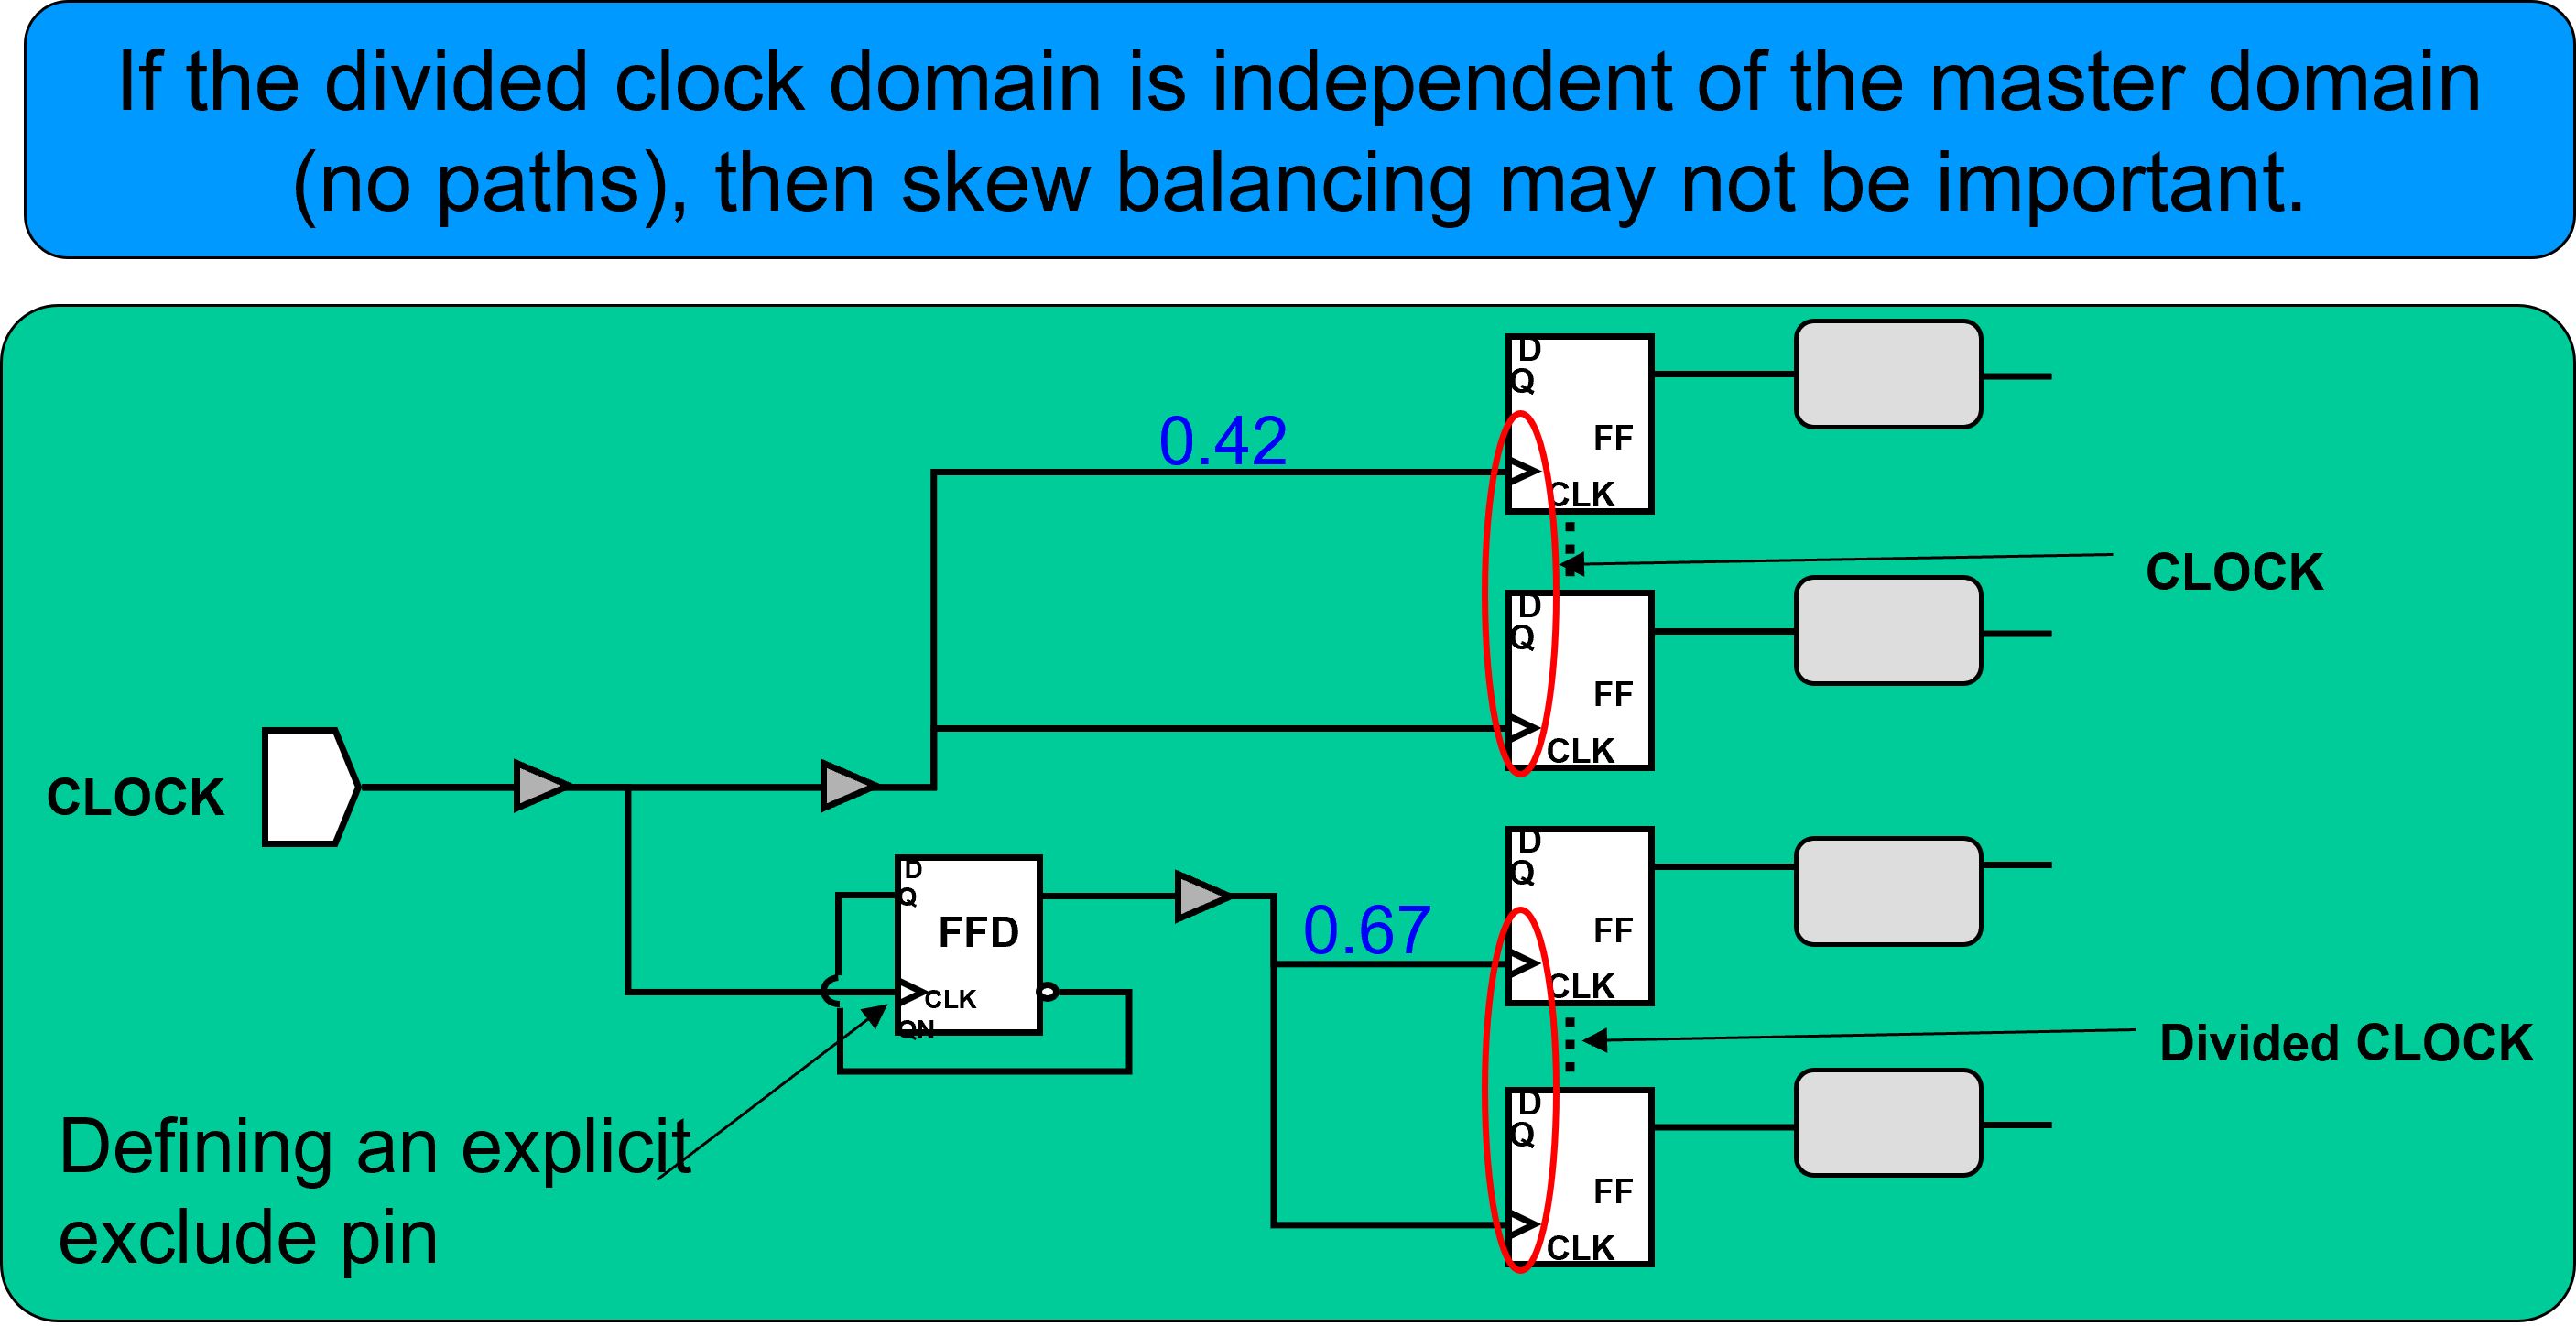
\includegraphics[width=\textwidth]{Balancing}
	\end{center}
\end{frame}

\begin{frame}
	\frametitle{No Inter-Clock Skew Balancing by Default}
	\begin{center}
		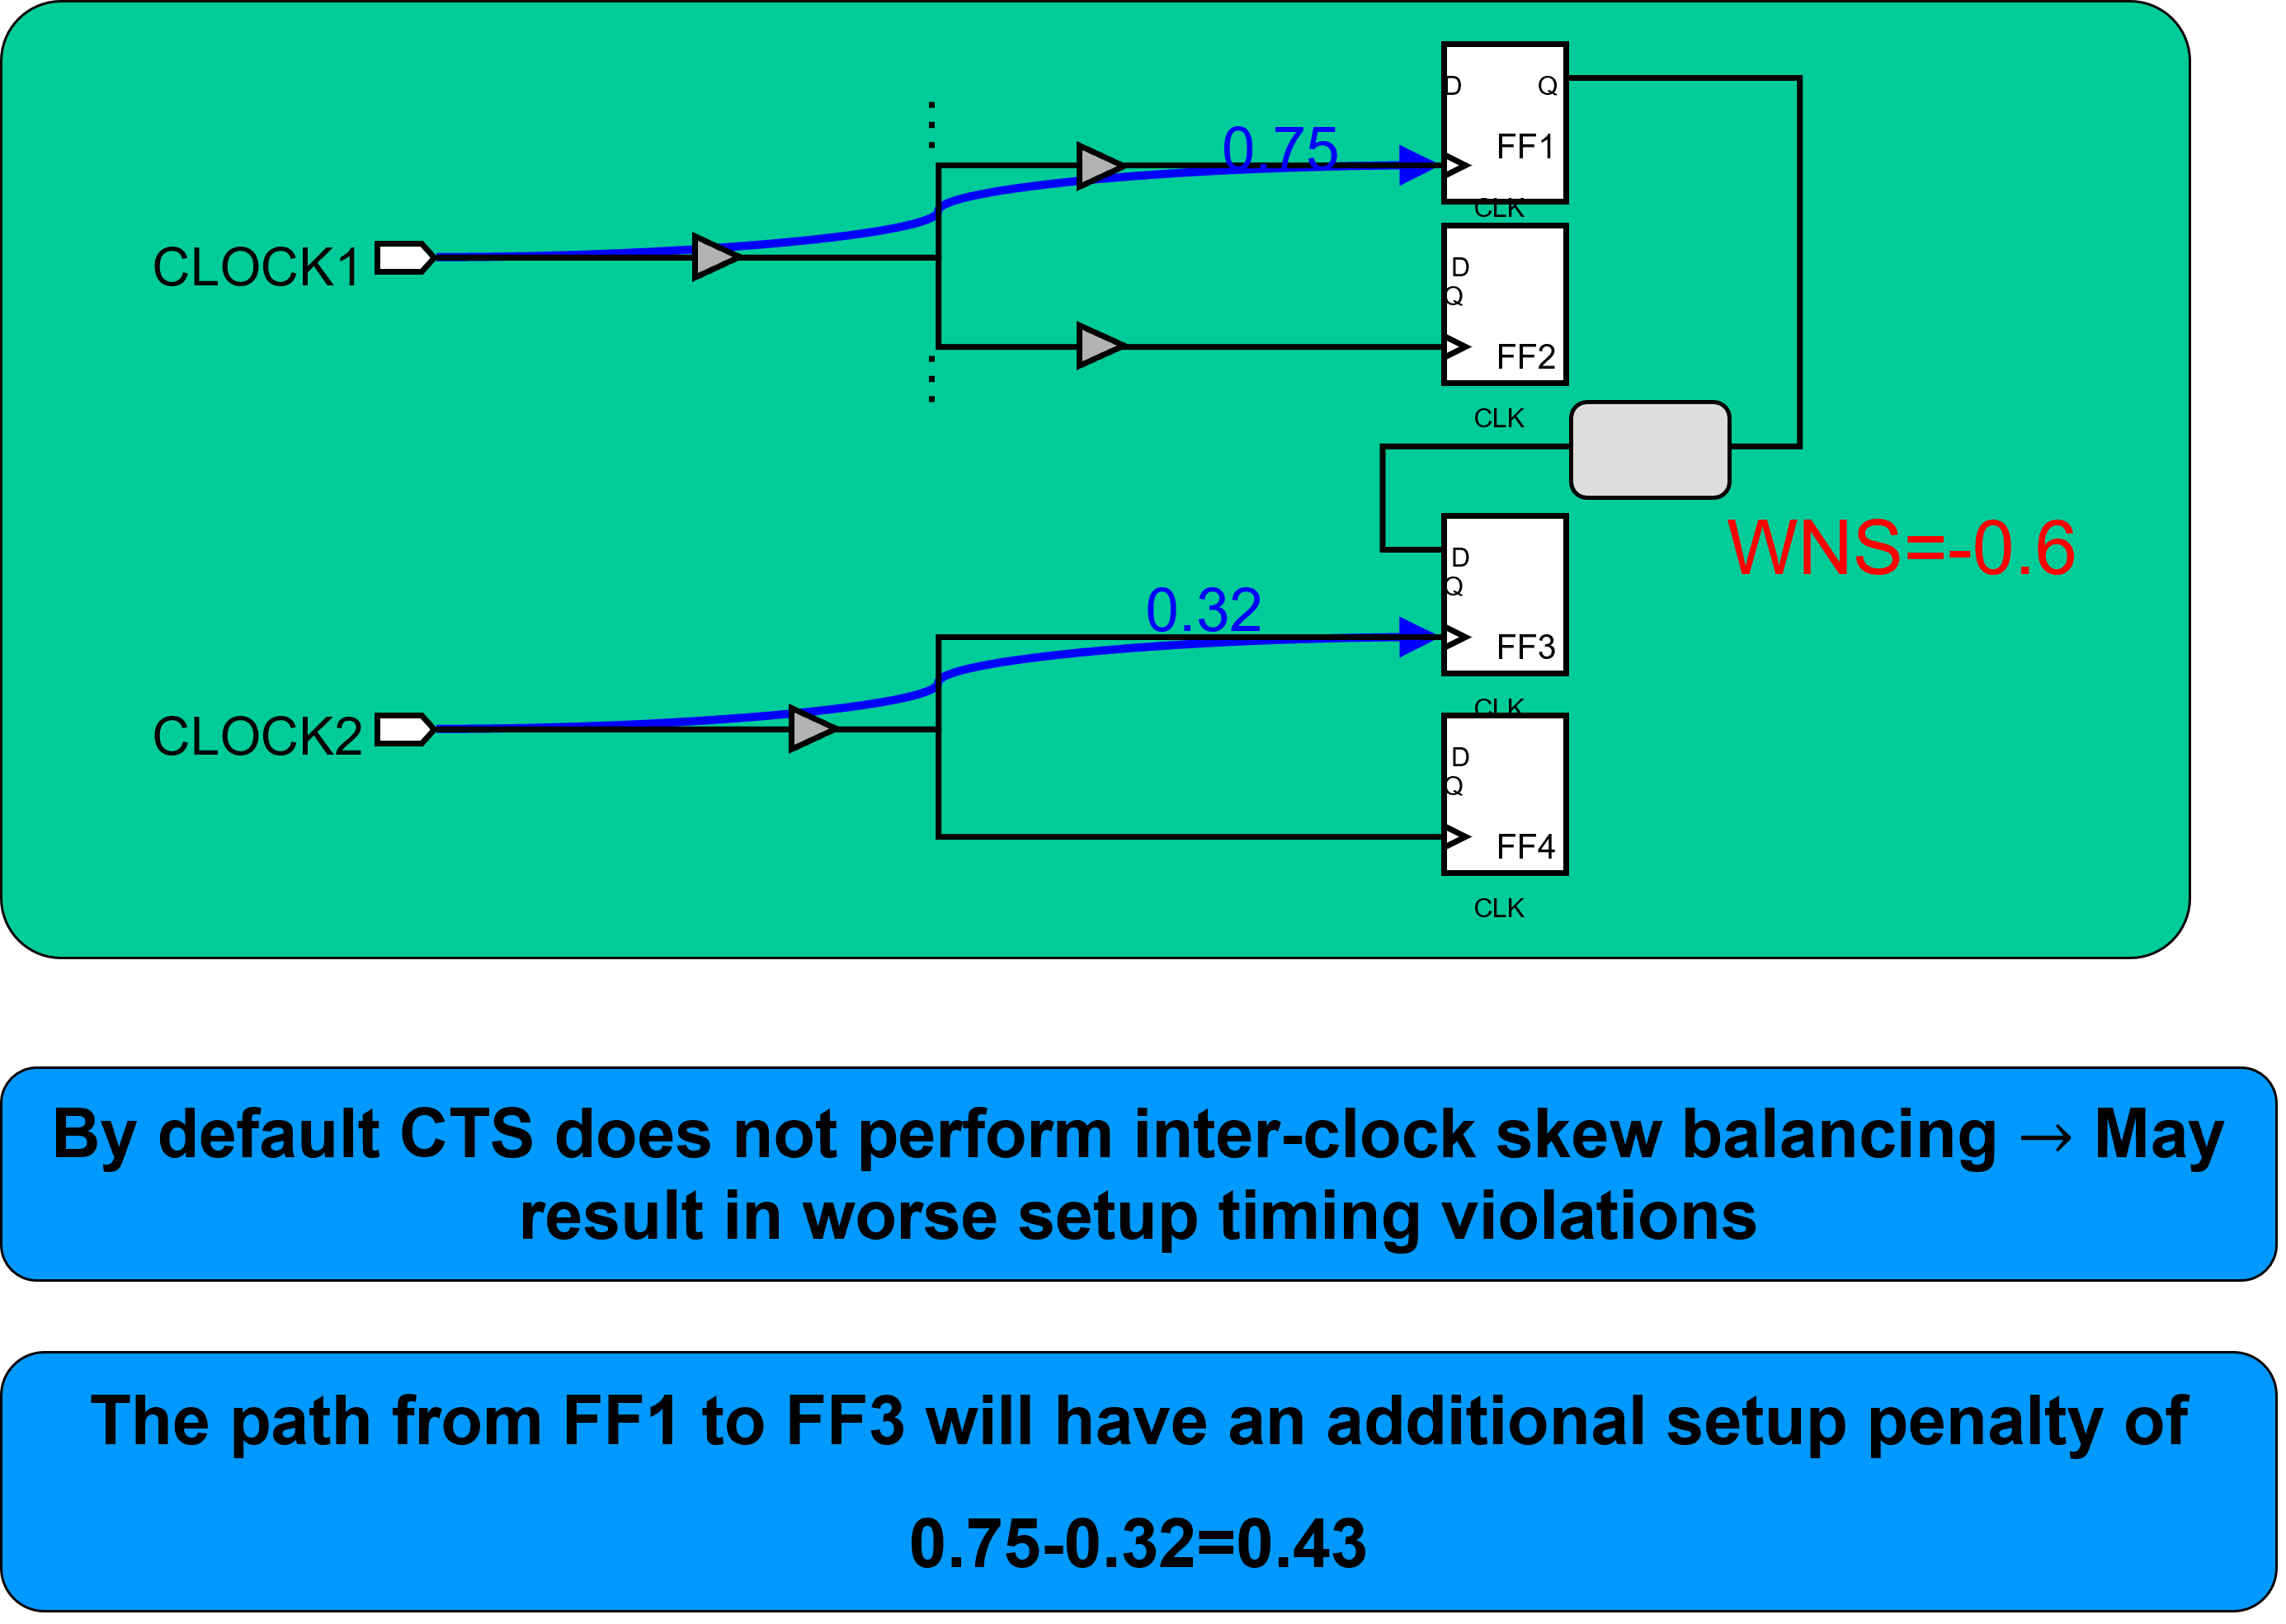
\includegraphics[width=\textwidth]{Inter-Clock}
	\end{center}
\end{frame}
\begin{frame}
	\frametitle{Inter-Clock Delay Balancing}
	\begin{center}
		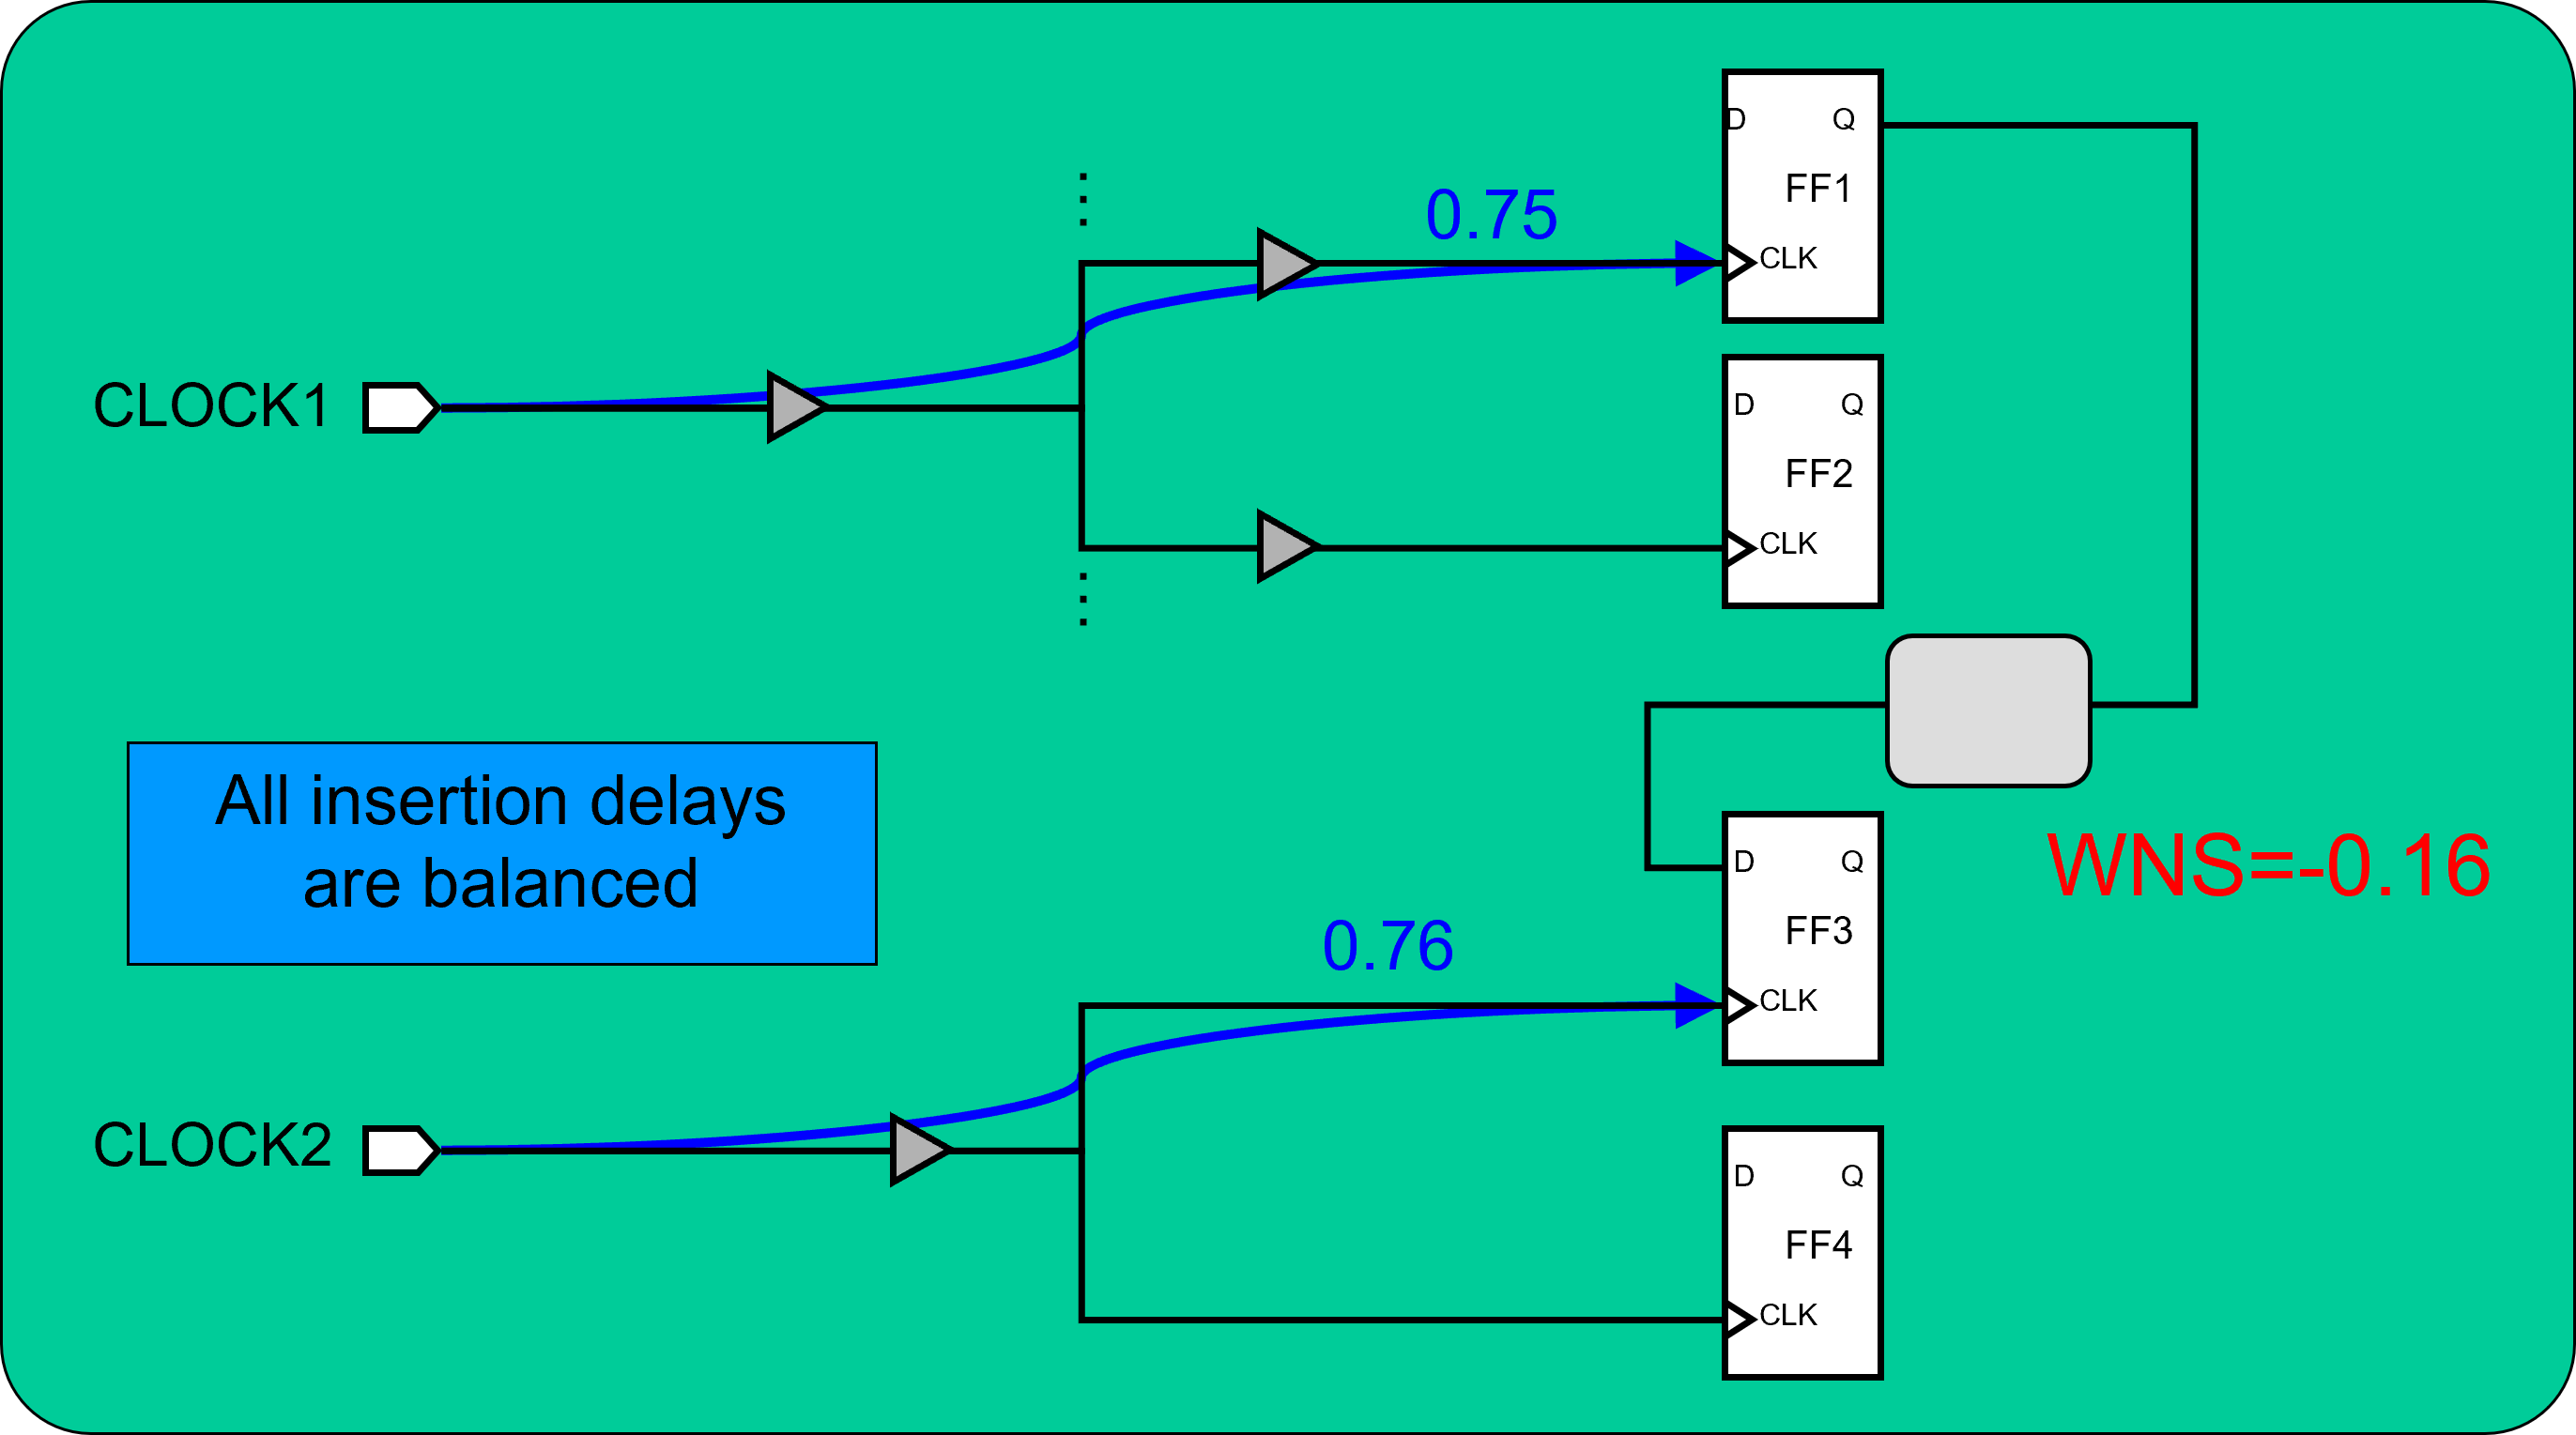
\includegraphics[width=\textwidth]{Inter-Clock1}
	\end{center}
\end{frame}
\begin{frame}
	\frametitle{Inter-Clock Delay Balancing: With Offset}
	\begin{center}
		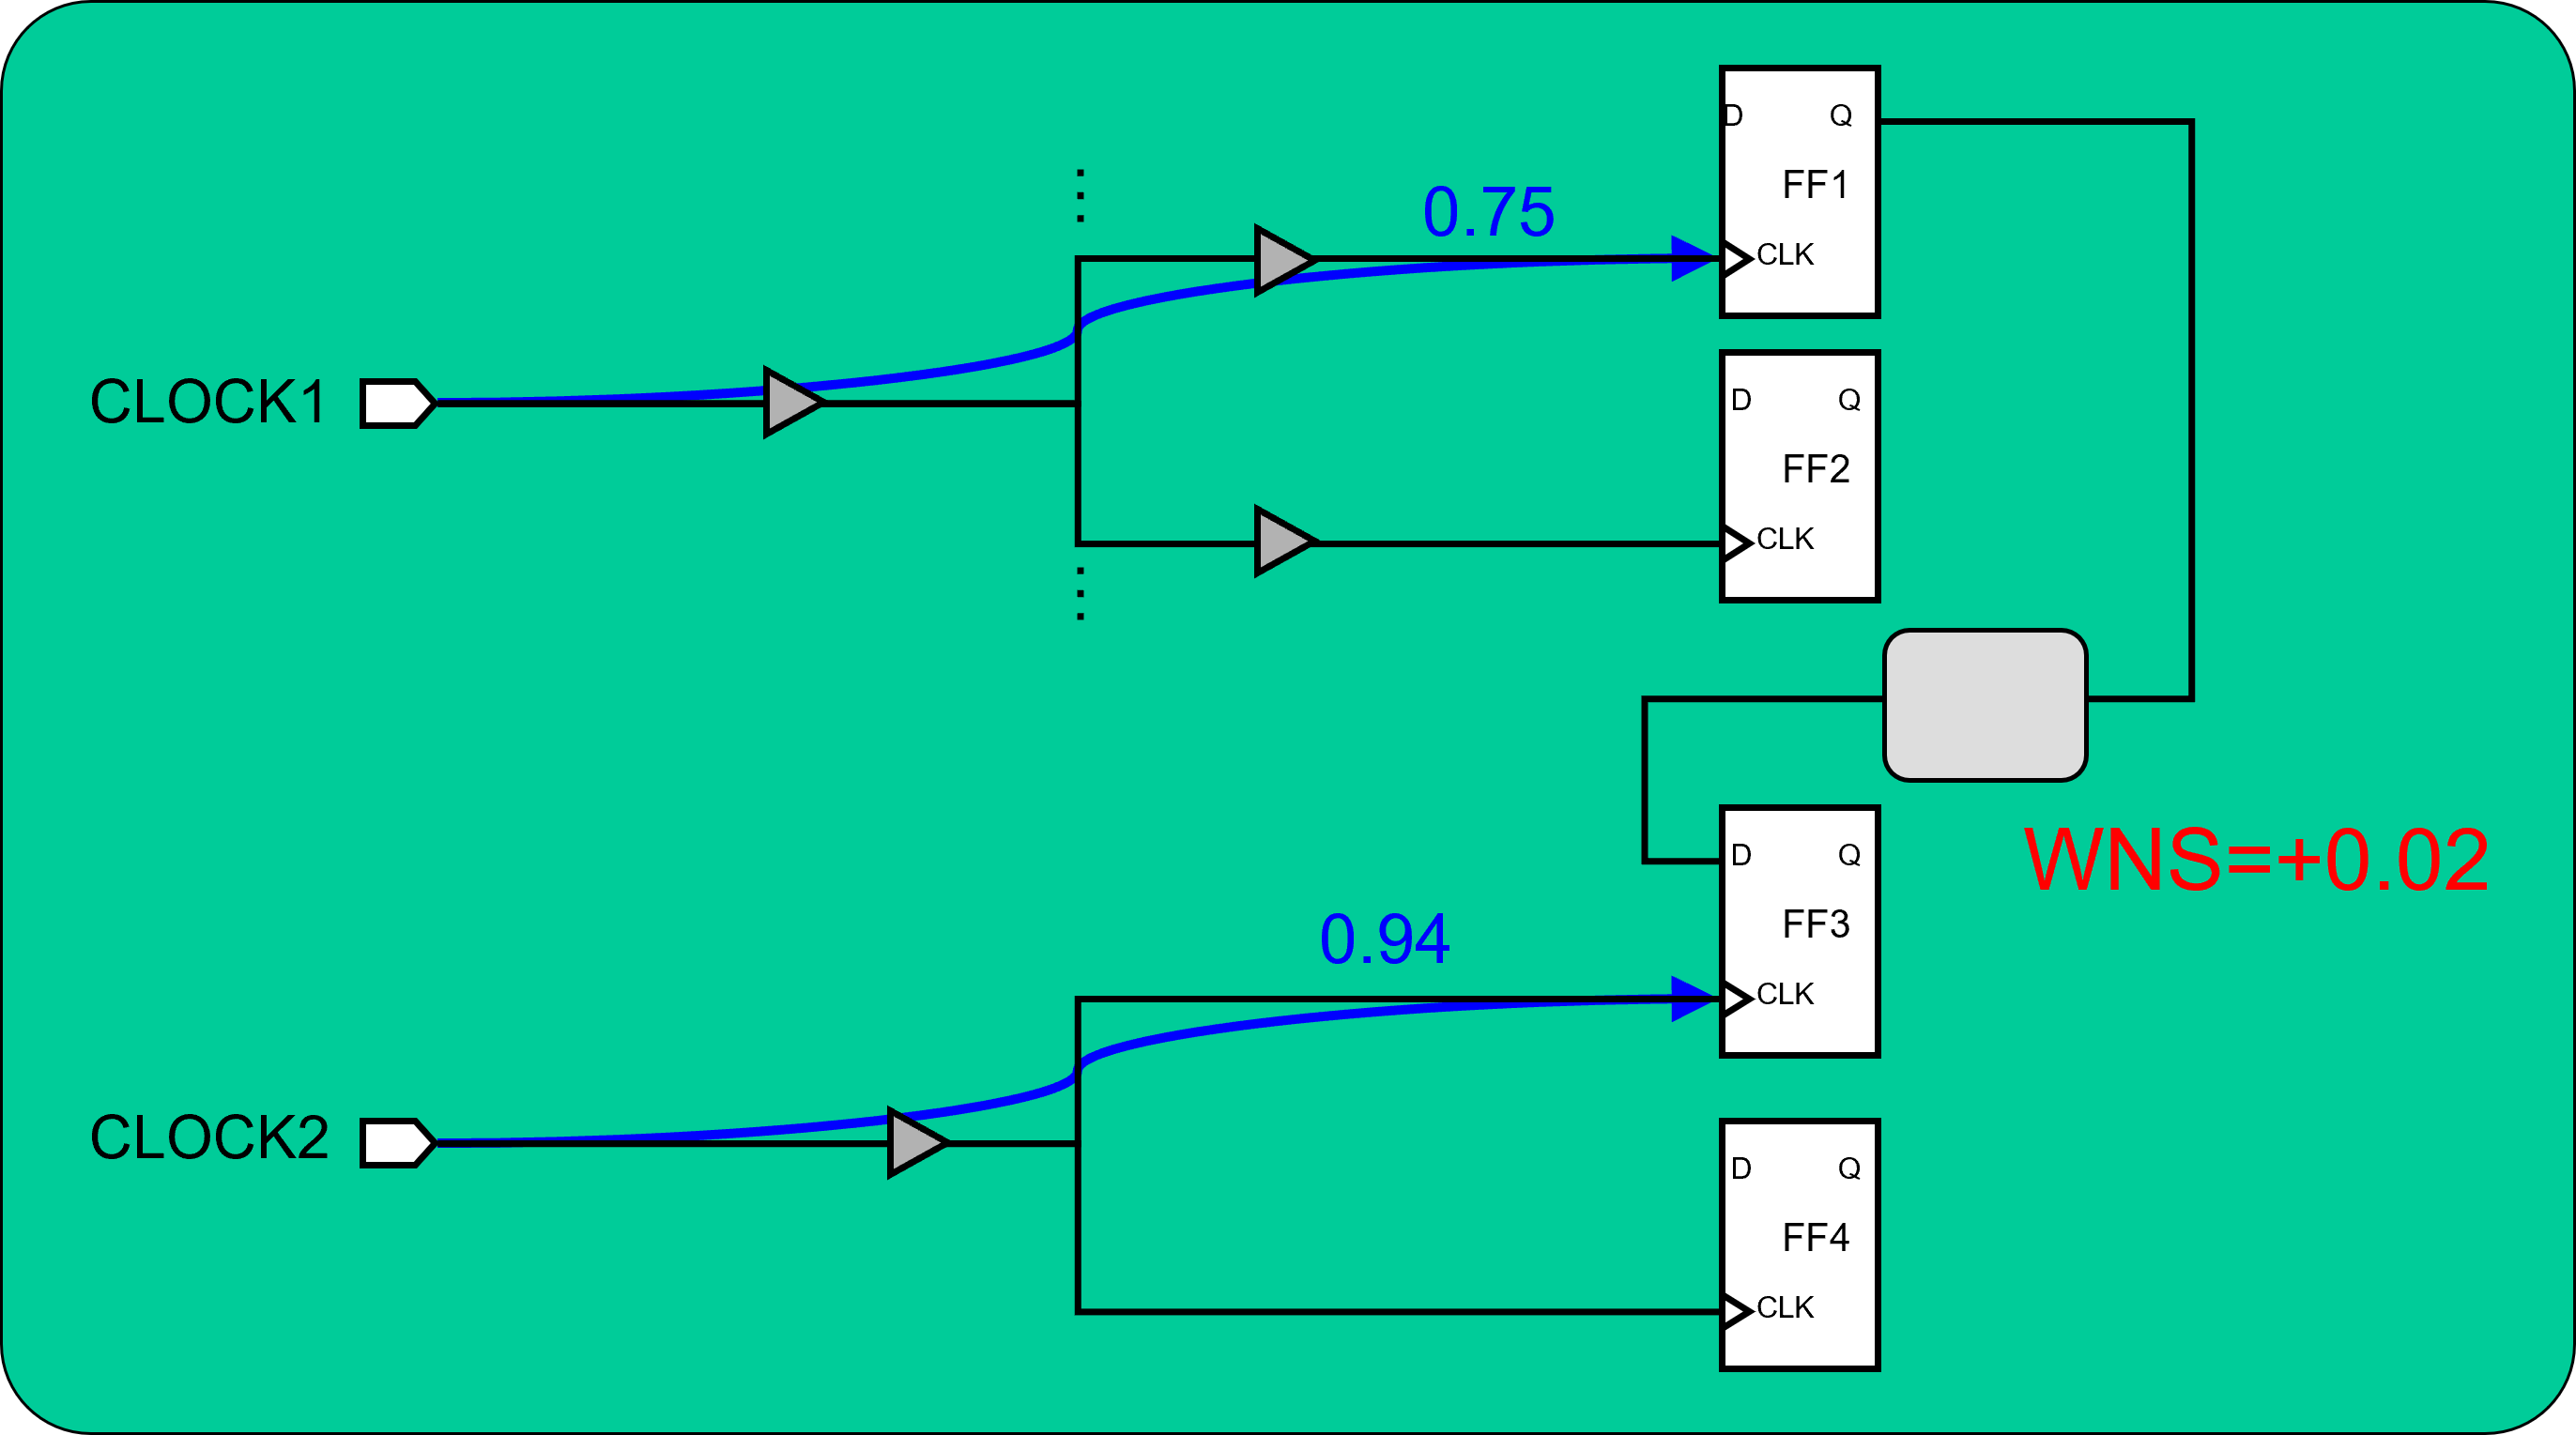
\includegraphics[width=\textwidth]{Inter-Clock2}
	\end{center}
\end{frame}

\begin{frame}
	\frametitle{User-defined or Explicit Stop Pins}
	\begin{center}
		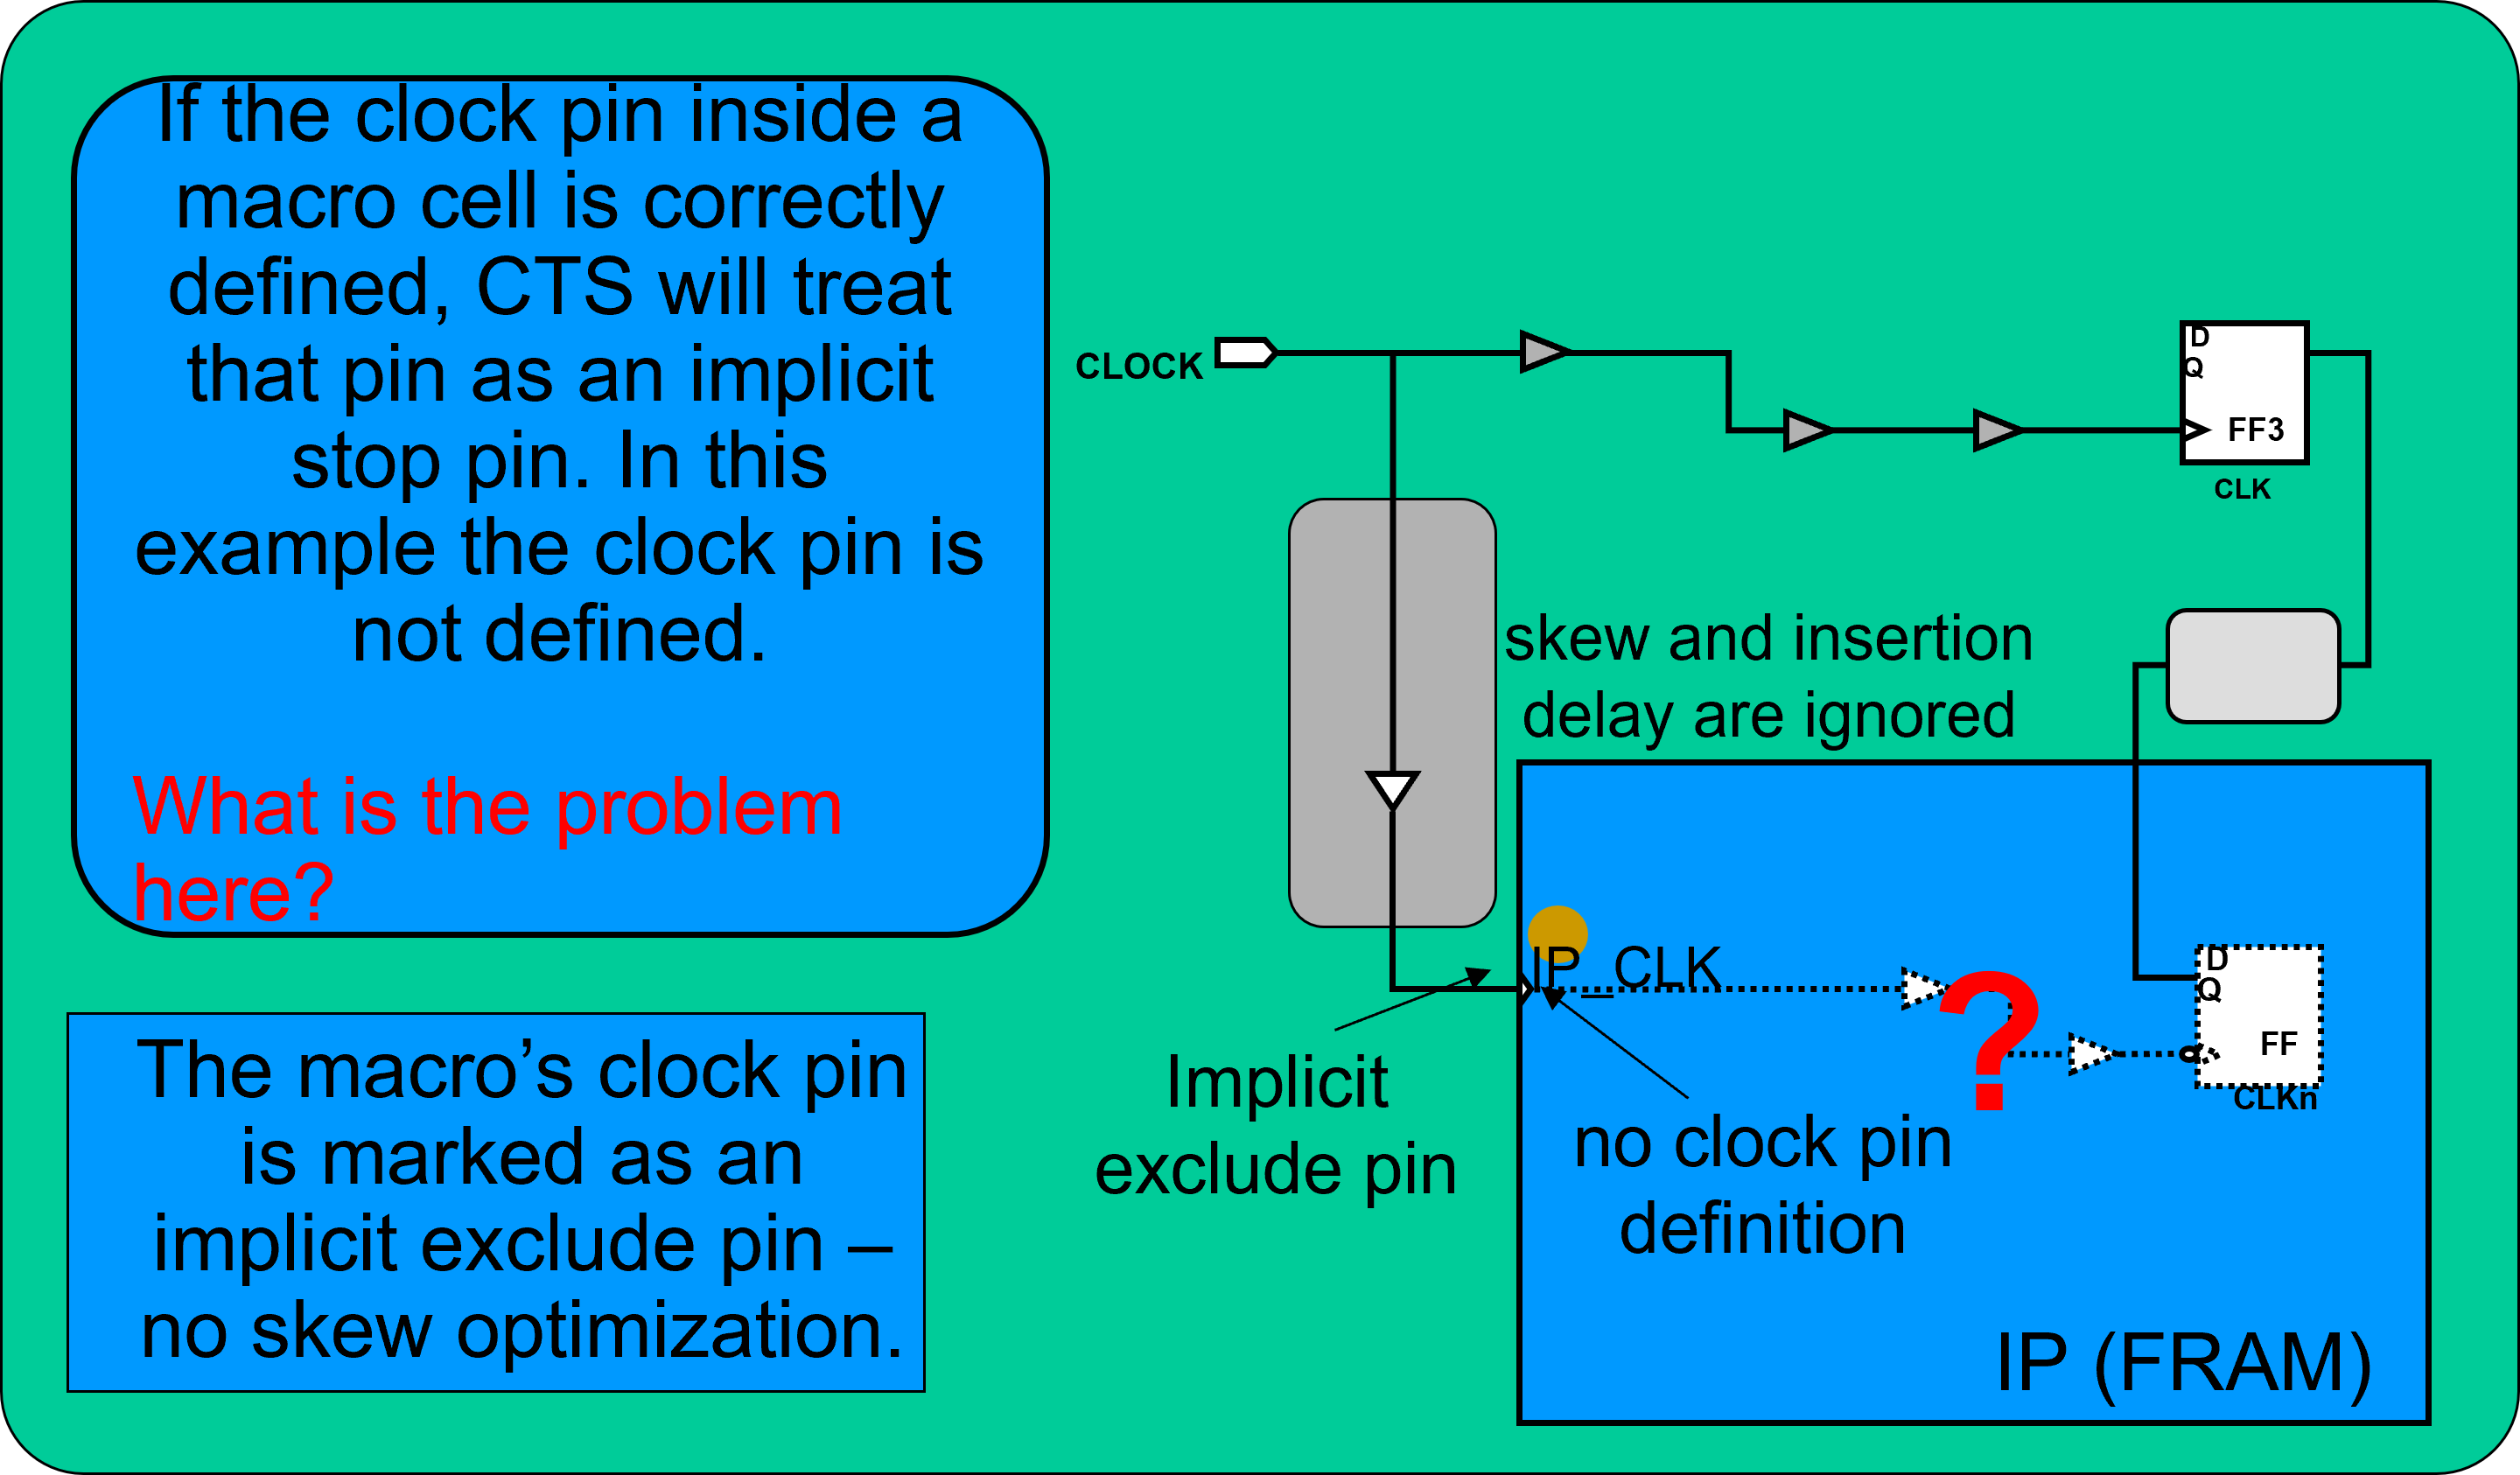
\includegraphics[width=\textwidth]{Stop}
	\end{center}
\end{frame}

\begin{frame}
	\frametitle{Defining an Explicit Stop Pin}
	\begin{center}
		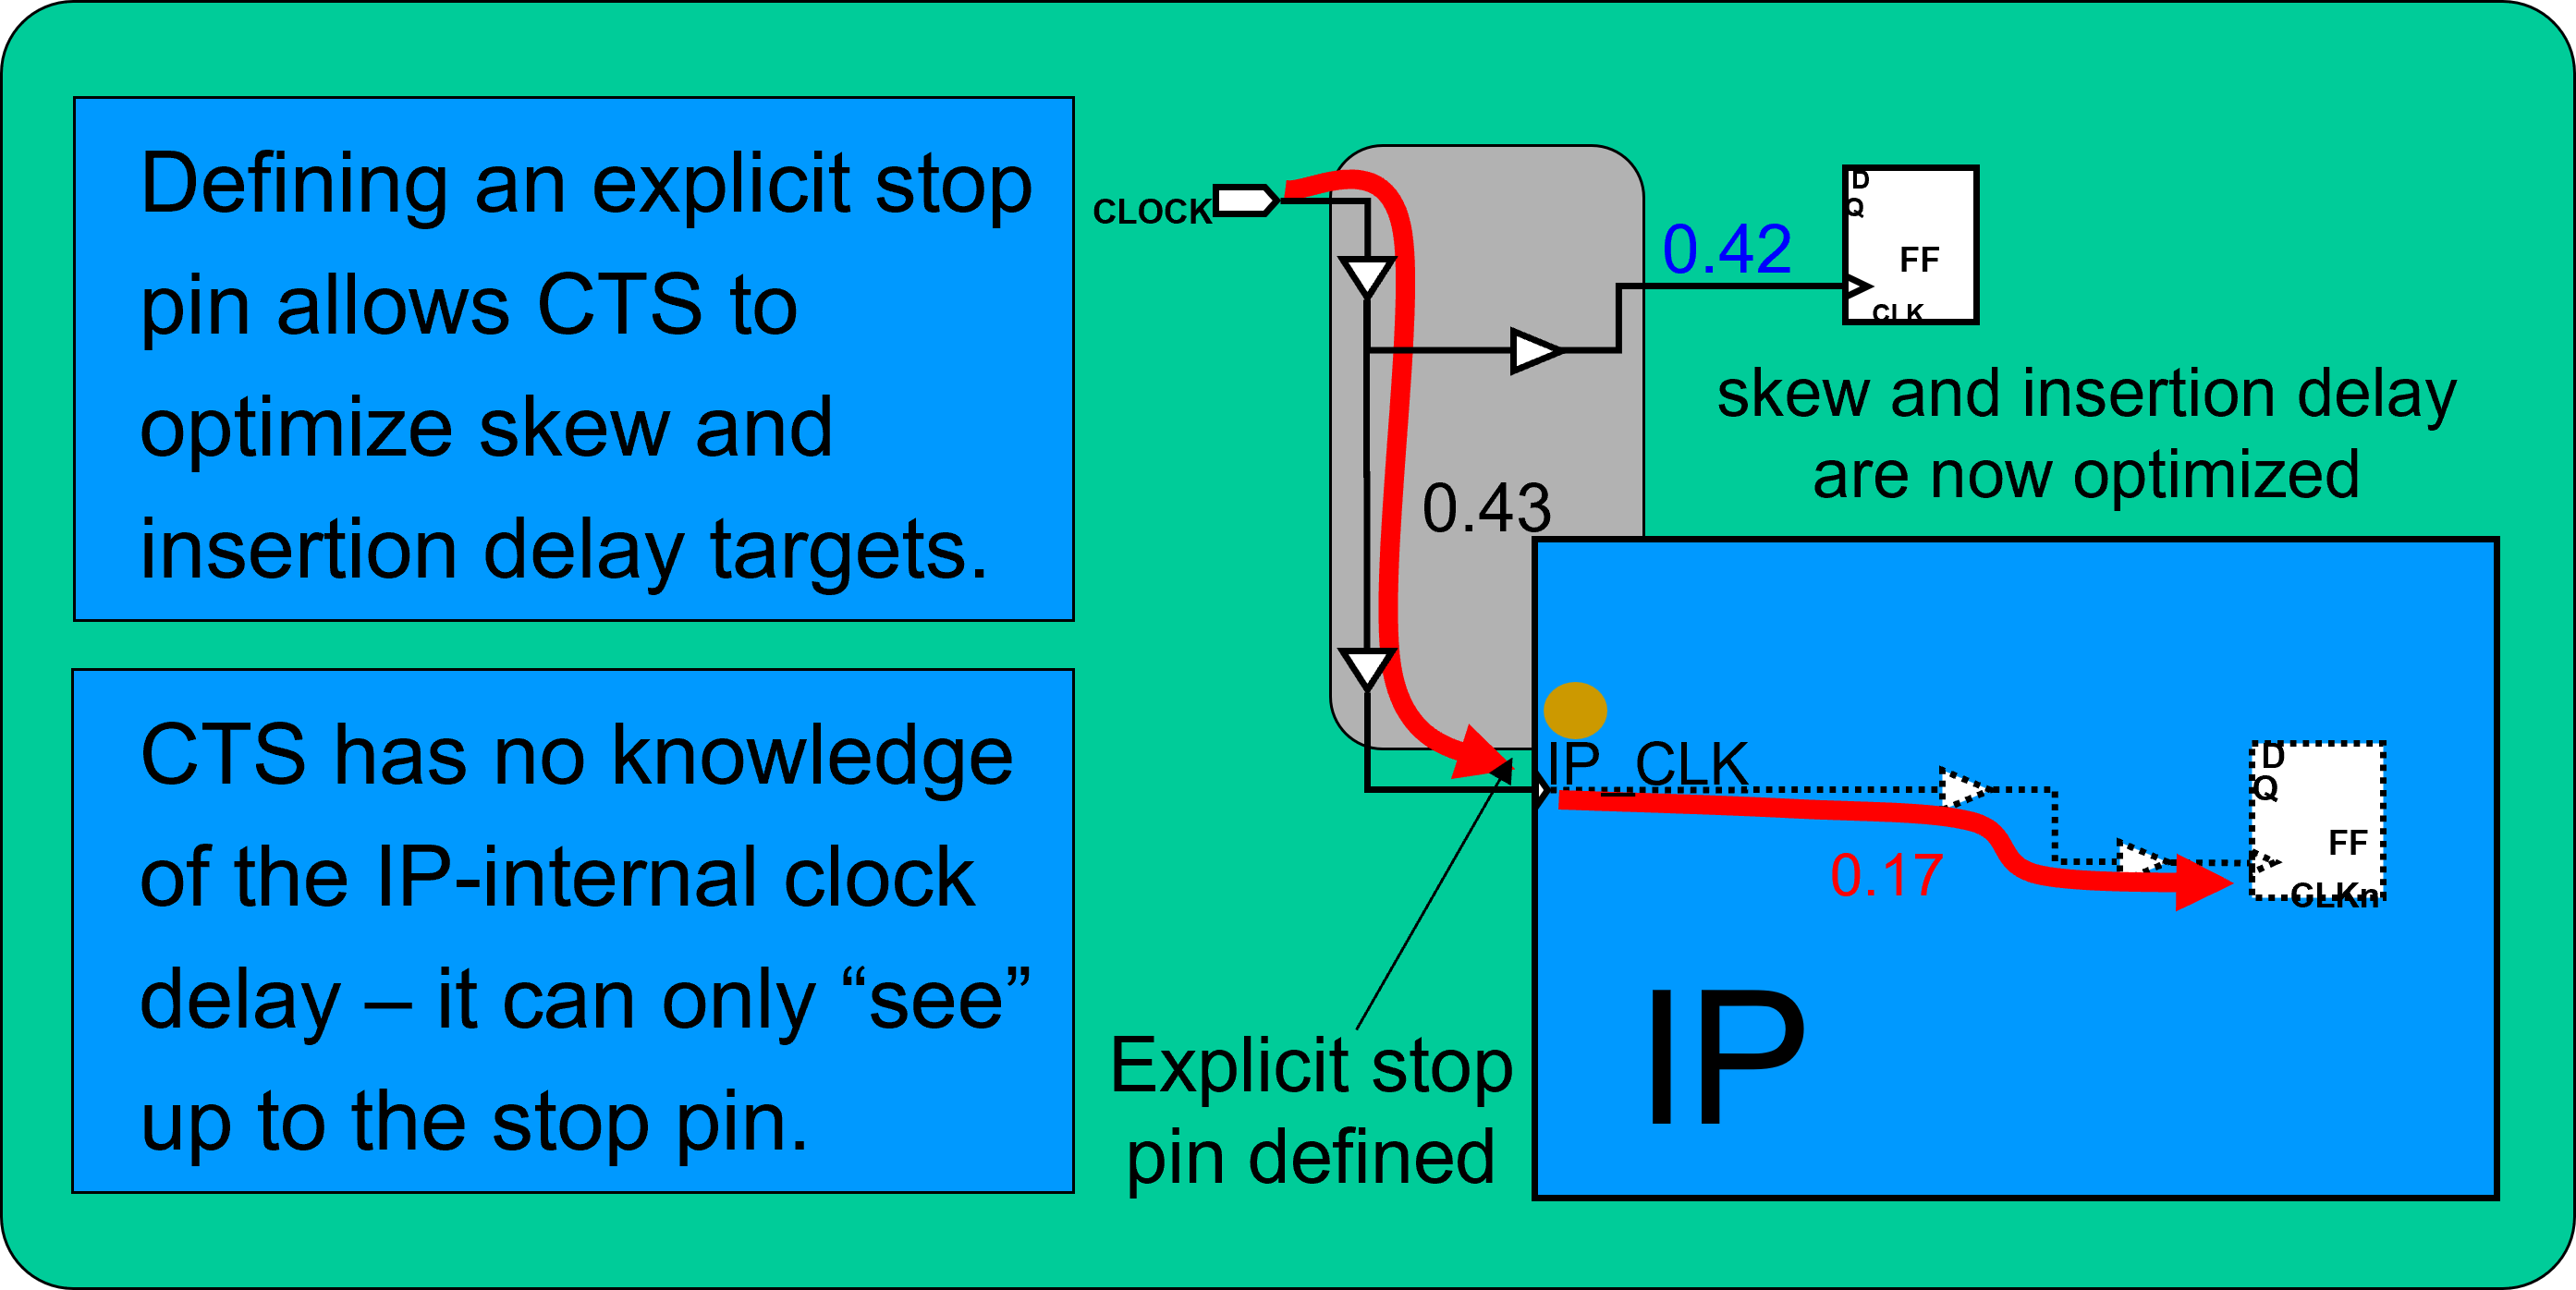
\includegraphics[width=\textwidth]{Stop1}
	\end{center}
\end{frame}

\begin{frame}
	\frametitle{Defining an Explicit Float Pin}
	\begin{center}
	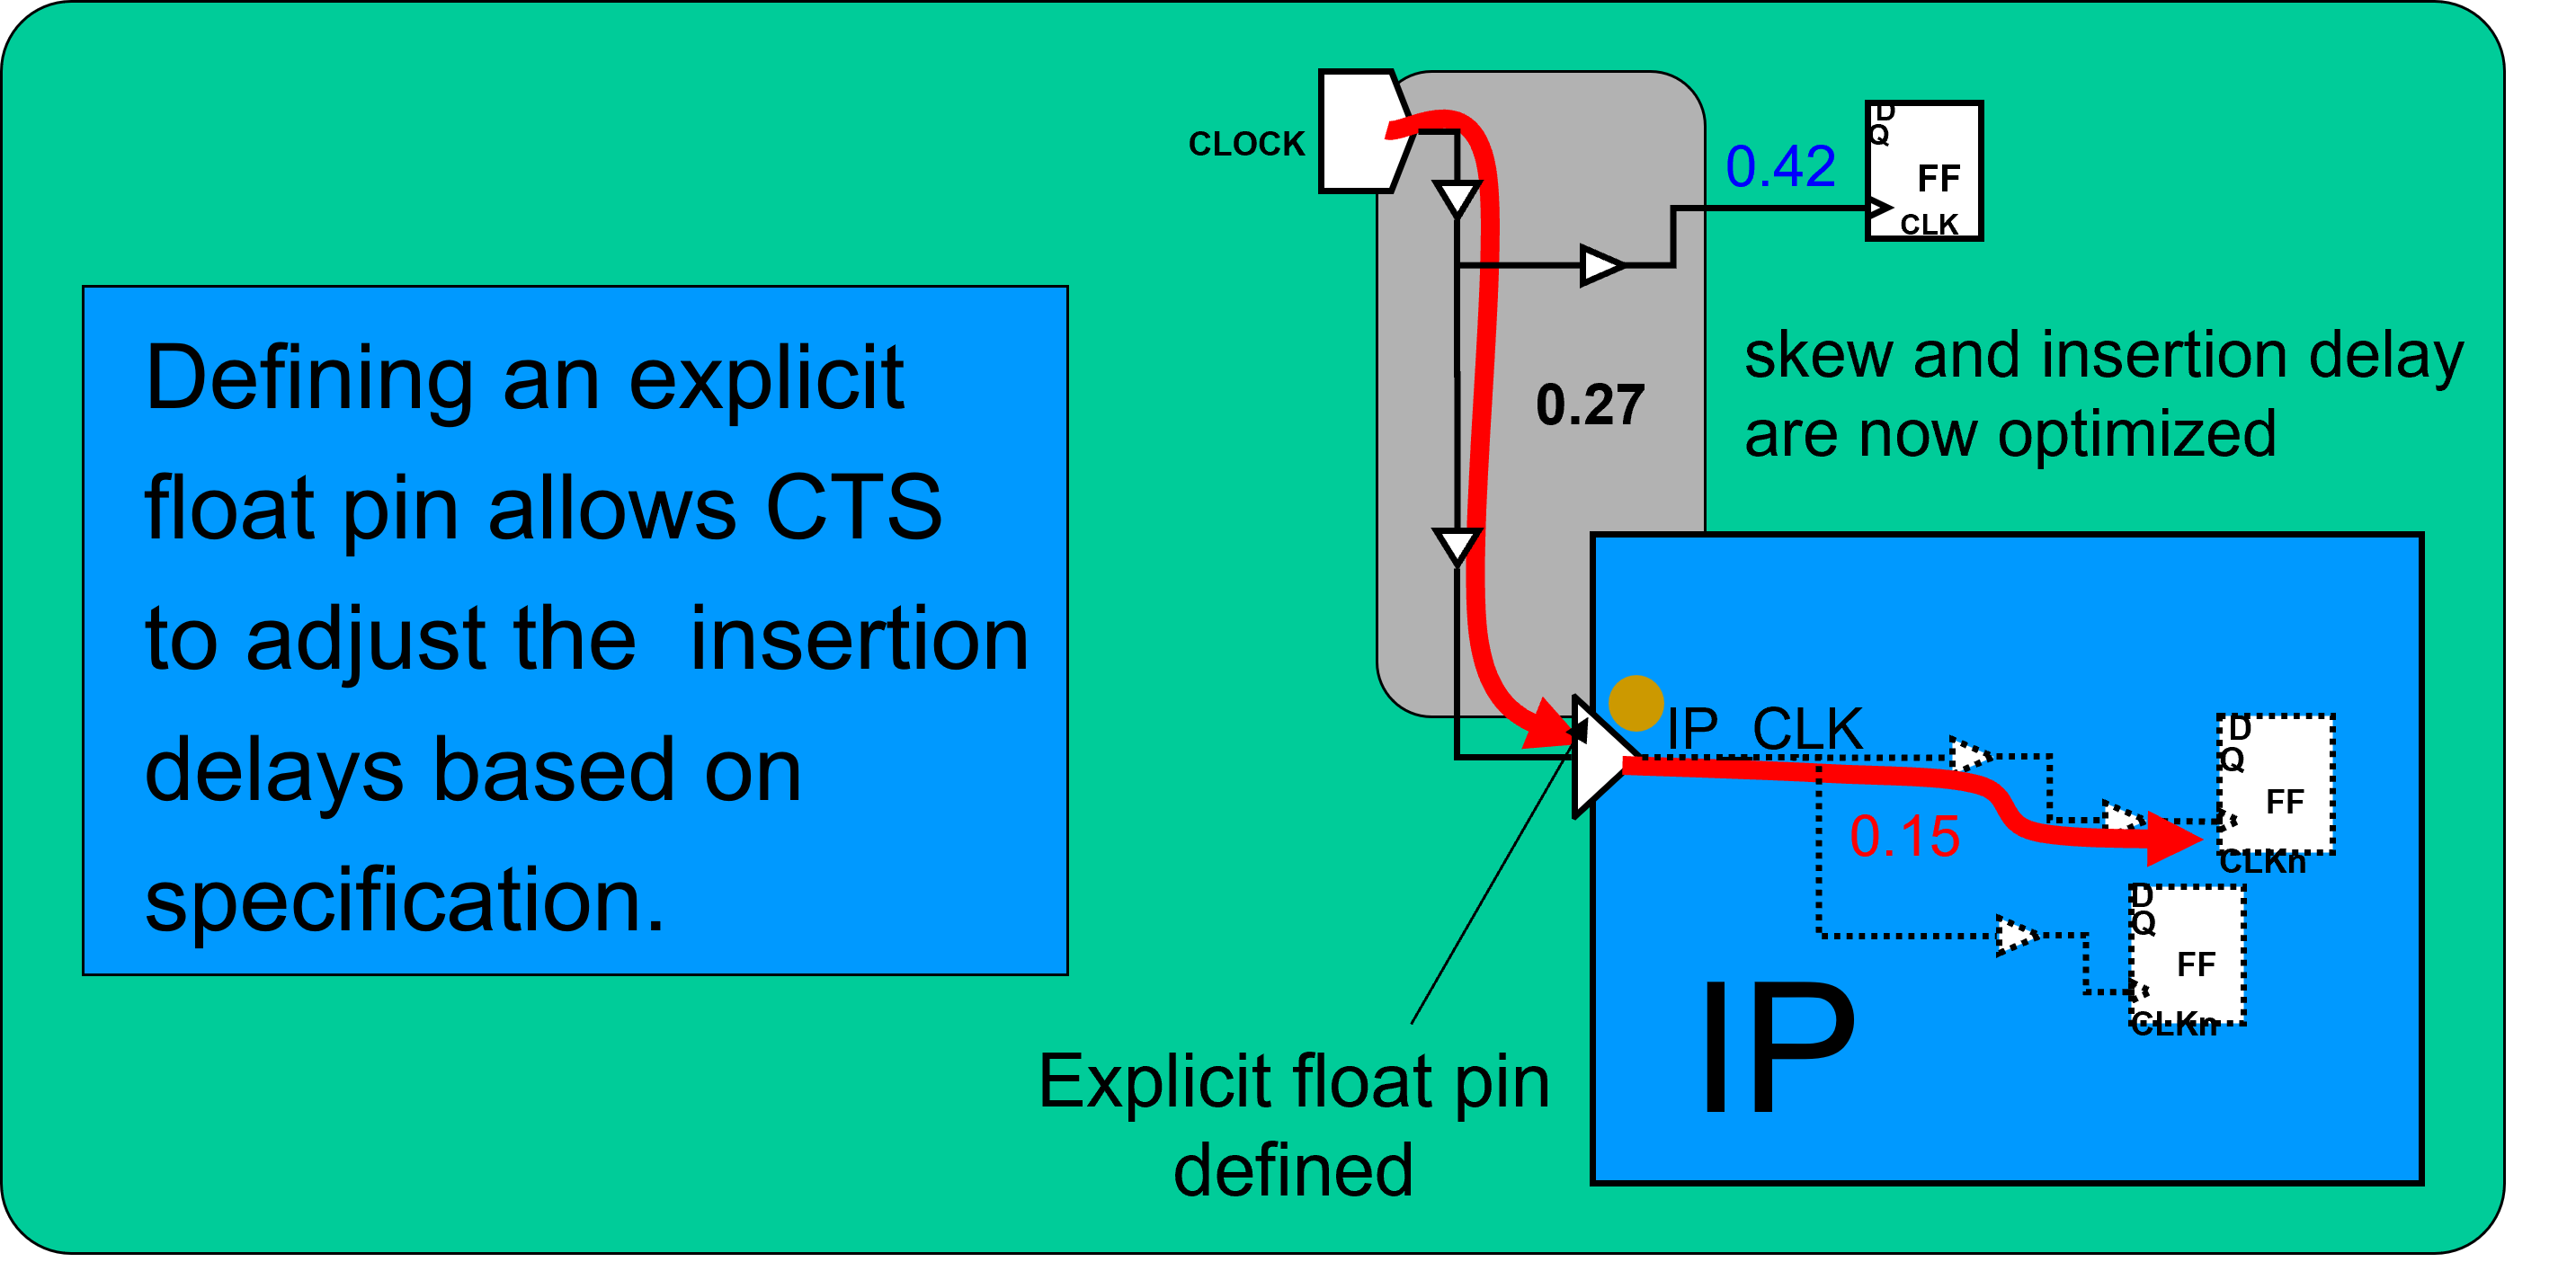
\includegraphics[width=\textwidth]{Float}
	\end{center}	
\end{frame}

\subsection[NDR]{Non-Default Clock Routing}
\begin{frame}
	\frametitle{Non-Default Clock Routing}
	\begin{itemize}
		\item PnR Tool can route the clocks using non-default routing rules, e.g. double-spacing, double-width, shielding, and double via
		\item Non-default rules are often used to “harden” the clock, e.g. to make the clock routes less sensitive to Cross Talk or EM effects, which improve yield
	\end{itemize}
	\begin{center}
		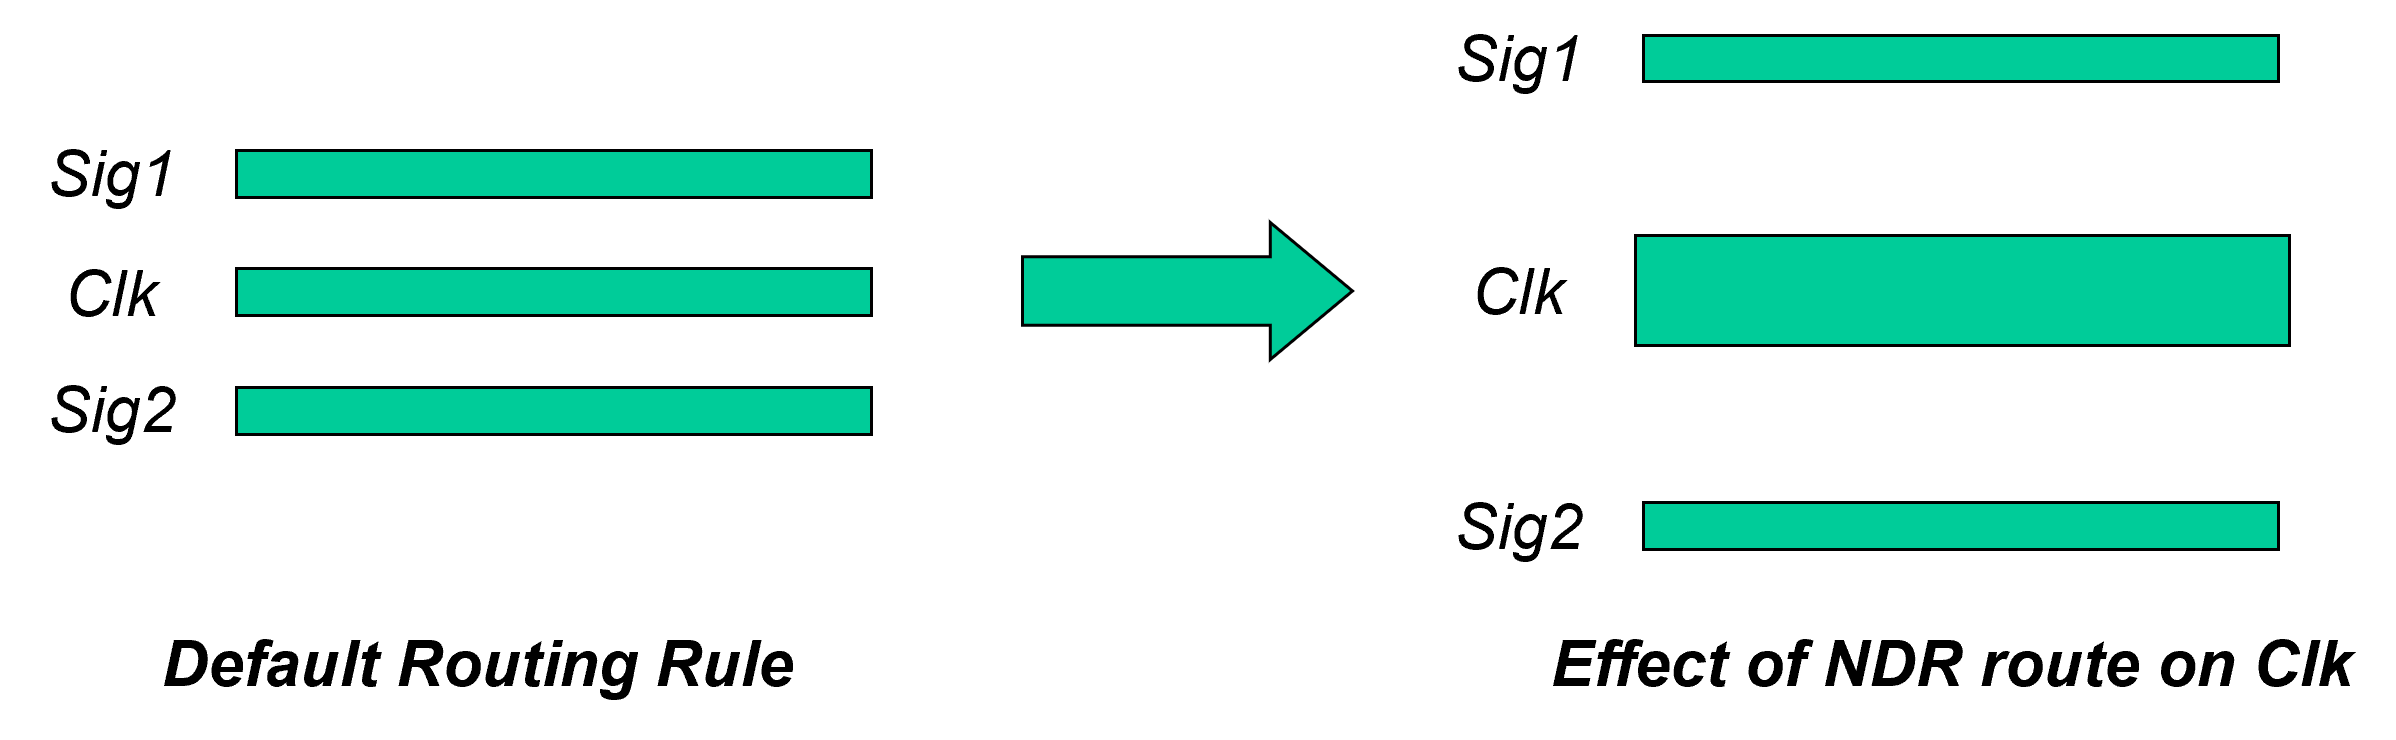
\includegraphics[width=0.7\textwidth]{NDR}
	\end{center}
\end{frame}

\begin{frame}
	\frametitle{NDR Recommendations}
	\begin{itemize}
		\item \textbf{Always route clock on metal 3 and above}
		\item \textbf{Avoid NDR on Metal 1}
		\begin{itemize}
			\item may have trouble accessing metal 1 pins on buffers and gates
		\end{itemize}
		\item \textbf{Consider using double spacing to reduce crosstalk}
		\item \textbf{Consider double width to reduce resistance}
		\item \textbf{Consider double via to reduce resistance and improve yield}
	\end{itemize}
\end{frame}

\begin{frame}
	\frametitle{Put NDR on Pitch for Accurate RC Estimation}
	\begin{itemize}
		\item \textbf{Metal traces are always routed “on pitch”}
		\item \textbf{With clock NDR rules, pre-routing RC estimates of
		clock nets use NDR width and spacing numbers}
		\item \textbf{If NDR [spacing + width] numbers are not integer
		multiples of pitch (i.e. off-pitch), timing estimates pre-route may not correlate well with post-route timing}
		\item \textbf{Make sure your NDR numbers are on pitch!}
	\end{itemize}
\end{frame}

\section[CTO]{Clock Tree Optimization}
\subsection[CTO]{Clock Tree Optimization }
\begin{frame}
	\frametitle{Clock Tree Optimization}
	\textbf{Perform additional Clock Tree Optimization as necessary to further improve clock skew.}
	\begin{center}
		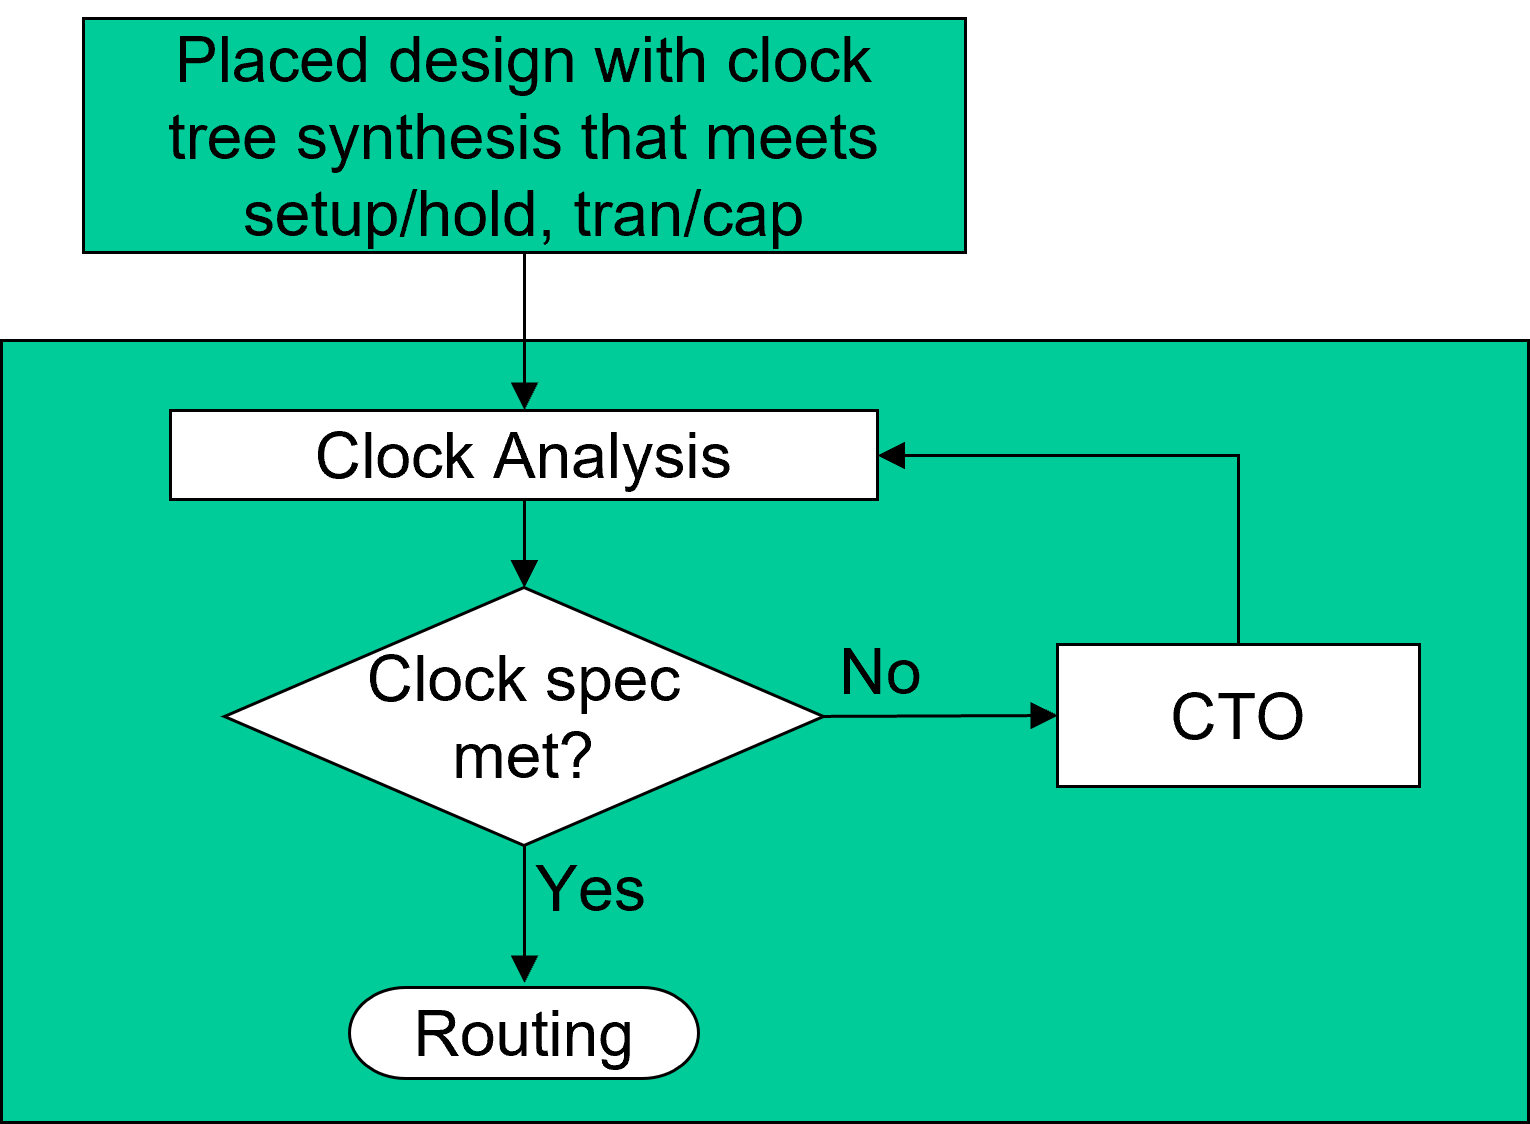
\includegraphics[width=0.8\textwidth]{CTO}
	\end{center}
\end{frame}

\begin{frame}
	\frametitle{Clock Tree Optimization Options}
	\begin{center}
		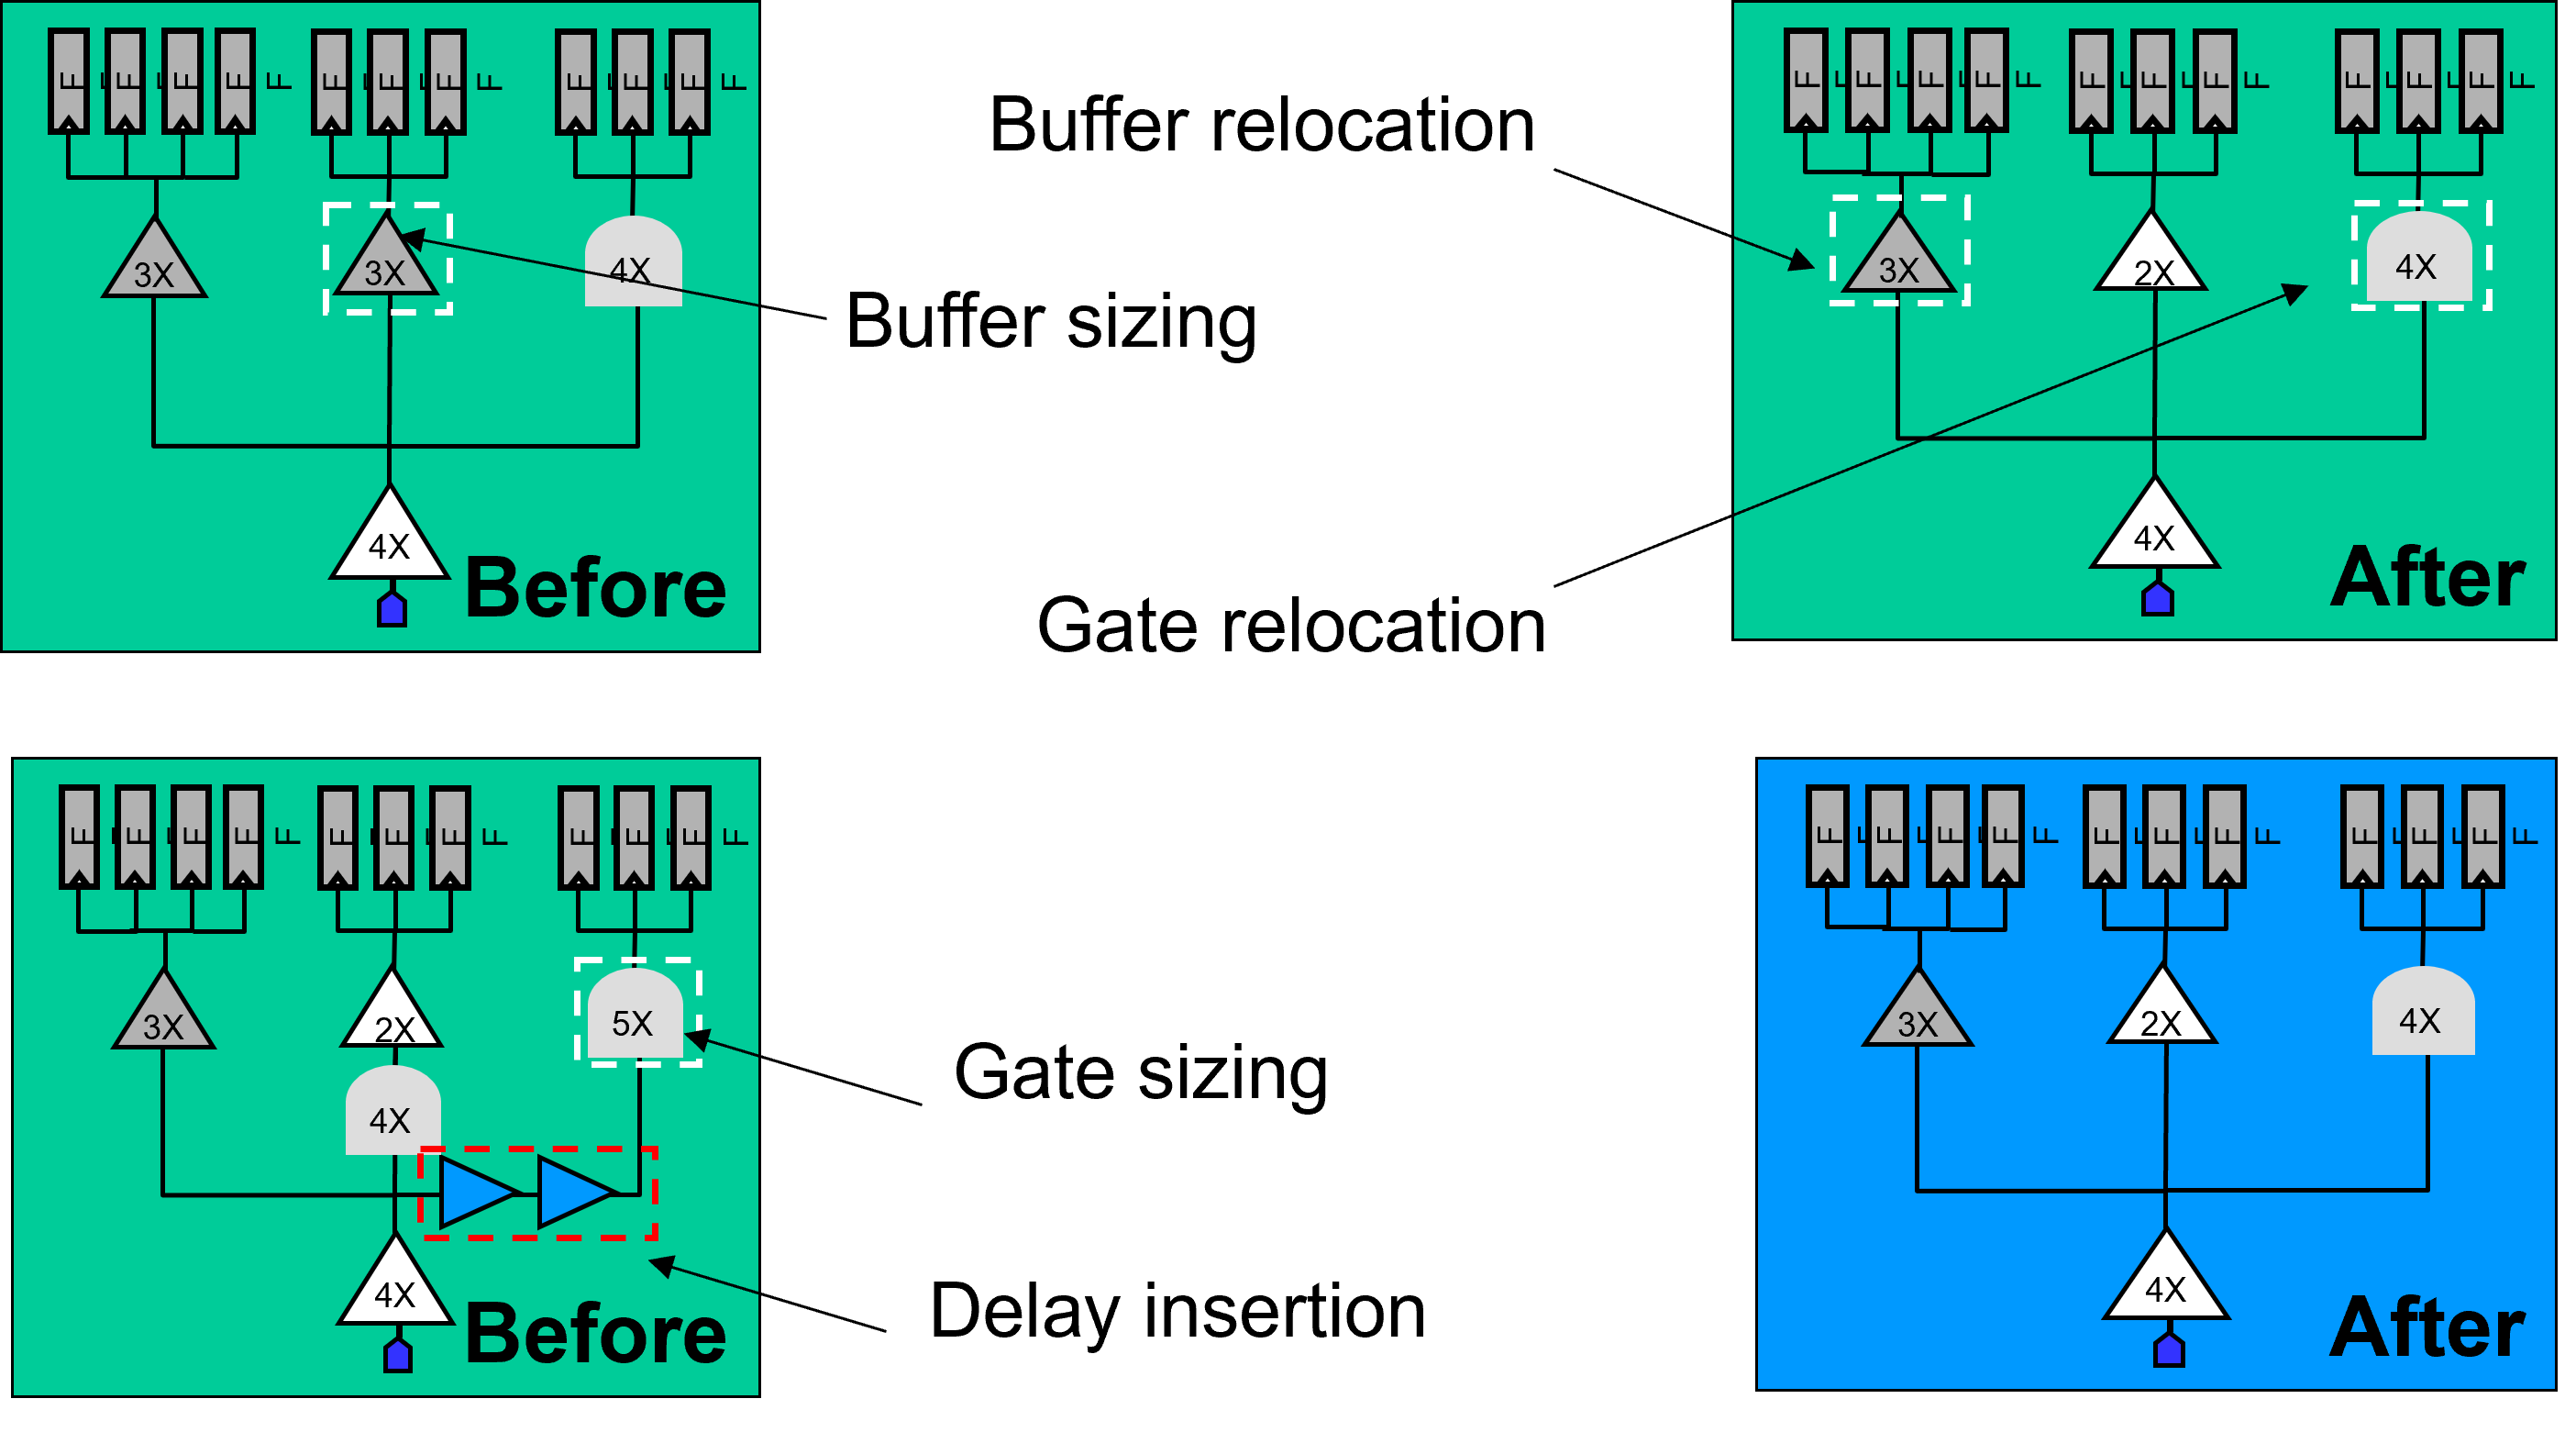
\includegraphics[width=\textwidth]{CTO1}
	\end{center}
\end{frame}

\subsection[Results]{Analyzing CTS Results}
\begin{frame}
	\frametitle{Analyzing CTS Results}
	\begin{itemize}
		\item Report clock tree 
		\begin{itemize}
			\item Summary
			\item Settings
			\item …
			\item Reports max global skew, late/early insertion delay, number of levels in clock tree, number of clock tree references (buffers), clock DRC violations
		\end{itemize}
		\item Report clock timing
		\begin{itemize}
			\item Reports actual, relevant skew, latency, interclock latency etc. for paths that are related
		\end{itemize}
	\end{itemize}
\end{frame}

\begin{frame}
	\frametitle{Effects of Clock Tree Synthesis}
	\begin{columns}	
		\column{0.6\textwidth}
		\begin{itemize}
			\item Clock buffers added
			\item Congestion may increase
			\item Non clock cells may have been moved to less ideal locations
			\item Inserting clock tress can introduce new timing and max tran/cap violations, which will be checked in the next stages
		\end{itemize}
		\column{0.6\textwidth}
		\begin{center}
			\includegraphics[width=0.7\textwidth]{CTS01}
		\end{center}
	\end{columns}
\end{frame}
%---------------------------------------------------	
\begin{frame}
	\frametitle{....}
	\begin{center}
		\<بِسْمِ اللَّـهِ الرَّحْمَـٰنِ الرَّحِيمِ> \\
		\<وَمَا أُوتِيتُمْ مِنَ الْعِلْمِ إِلَّا قَلِيلًا>
		
	\end{center}
\end{frame}
%---------------------------------------------	
\end{document}	